% 	TO DO: 
%	MZ Tabelle nicht einfügen: DDRD estimate von Regression mit 3 CG


%--------------------------------------------------------------------
%	DOCUMENT CLASS
%--------------------------------------------------------------------
\documentclass[11pt, a4paper, draft]{article} % type of document (paper, presentation, book,...); scrartcl class with sans serif titles, European layout 
\usepackage{fullpage} % leaves less space at margins of page
\usepackage[onehalfspacing]{setspace} % determine line pitch to 1.5

%--------------------------------------------------------------------
%	INPUT
%--------------------------------------------------------------------
\usepackage[T1]{fontenc} 	% Use 8-bit encoding that has 256 glyphs
\usepackage[utf8]{inputenc} % Required for including letters with accents, Umlaute,...
\usepackage{float} 			% better control over placement of tables and figures in the text
\usepackage{graphicx} 		% input of graphics
\usepackage{xcolor} 		% advanced color package
\usepackage{url} 			% include (clickable) URLs
\usepackage[breaklinks=true]{hyperref}
\usepackage{pdfpages}		% insert pages of external pdf documents
\setlength{\parskip}{0.75em}	% vertical spacing for paragraphs
\setlength{\parindent}{0em}	% horizonzal spacing for paragraphs
\usepackage{tikz}
\usepackage{tikzscale}		% helps to adjust tikz pictures to textwidth/linewidth
\usetikzlibrary{decorations.pathreplacing}
\usetikzlibrary{patterns}
\usetikzlibrary{arrows}
\usepackage{eurosym}		% Eurosymbol

% Have sections in TOC, but not in text
\usepackage{xparse}% for easier management of optional arguments
\ExplSyntaxOn
\NewDocumentCommand{\TODO}{msom}
{
	\IfBooleanF{#1}% do nothing if it's starred
	{
		\cs_if_eq:NNT #1 \chapter { \cleardoublepage\mbox{} }
		\refstepcounter{\cs_to_str:N #1}
		\IfNoValueTF{#3}
		{
			\addcontentsline{toc}{\cs_to_str:N #1}{\protect\numberline{\use:c{the\cs_to_str:N #1}}#4}
		}
		{
			\addcontentsline{toc}{\cs_to_str:N #1}{\protect\numberline{\use:c{the\cs_to_str:N #1}}#3}
		}
	}
	\cs_if_eq:NNF #1 \chapter { \mbox{} }% allow page breaks after sections
}
\ExplSyntaxOff

%--------------------------------------------------------------------
%	TABLES, FIGURES, LISTS
%--------------------------------------------------------------------
\usepackage{booktabs} 		% better tables
\usepackage{longtable}		% tables that may be continued on the next page
\usepackage{threeparttable} % add notes below tables
\renewcommand\TPTrlap{}		% add margins on the side of the notes
	\renewcommand\TPTnoteSettings{%
	\setlength\leftmargin{5 pt}%
	\setlength\rightmargin{5 pt}%
}
\usepackage[
center, format=plain,
font=normalsize,
nooneline,
labelfont={bf}
]{caption} 				% change format of captions of tables and graphs 
%USED IN MPHIL: \usepackage[labelfont=bf,labelsep = period, singlelinecheck=off,justification=raggedright]{caption}, other specifications which are nice: labelformat = parens -> number in paranthesis 


%\usepackage{threeparttablex} % for "ThreePartTable" environment, helps to combine threepart and longtable

% Allow line breaks with \\ in column headings of tables
\newcommand{\clb}[3][c]{%
	\begin{tabular}[#1]{@{}#2@{}}#3\end{tabular}}

% allow line breaks with \\ in row titles
\usepackage{multirow}

\newcommand{\rlb}[3][c]{%
\multirow{2}{*}{\begin{tabular}[#1]{@{}#2@{}}#3\end{tabular}}}% optional argument: b = bottom or t= top alignment


\usepackage[singlelinecheck=on]{subcaption}%both together help to have subfigures
\usepackage{wrapfig}				% wrap text around figure


\usepackage{rotating}				% rotating figures & tables
\usepackage{enumerate}				% change appearance of the enumerator
\usepackage{paralist, enumitem}		% better enumerations
\setlist{noitemsep}					% no additional vertical spacing for enurations
%--------------------------------------------------------------------
%	MATH
%--------------------------------------------------------------------
\usepackage{amsmath,amssymb,amsfonts} % more math symbols and commands
\let\vec\mathbf				 % make vector bold, with no arrow and not in italic

%--------------------------------------------------------------------
%	LANGUAGE SPECIFICS
%--------------------------------------------------------------------
\usepackage[american]{babel} % man­ages cul­tur­ally-de­ter­mined ty­po­graph­i­cal (and other) rules, and hy­phen­ation pat­terns
\usepackage{csquotes} % language specific quotations

%--------------------------------------------------------------------
%	BIBLIOGRAPHY & CITATIONS
%--------------------------------------------------------------------
\usepackage{csquotes} % language specific quotations
\usepackage{etex}		% some more Tex functionality
\usepackage[nottoc]{tocbibind} %add bibliography to TOC
\usepackage[authoryear, round, comma]{natbib} %biblatex

%--------------------------------------------------------------------
%	PATHS
%--------------------------------------------------------------------
\makeatletter
\def\input@path{{../../analysis/tables/}}	%PATH TO TABLES
%or: \def\input@path{{/path/to/folder/}{/path/to/other/folder/}}
\makeatother
\graphicspath{{../../analysis/graphs/}}		% PATH TO GRAPHS

%--------------------------------------------------------------------
%	LAYOUT
%--------------------------------------------------------------------
\usepackage[left=3cm,right=3cm,top=2cm,bottom=3cm]{geometry}
\usepackage{pdflscape} % lscape.sty Produce landscape pages in a (mainly) portrait document.

\definecolor{darkblue}{rgb}{0.0,0.0,0.6}
\newcommand\natalia[1]{\textcolor{orange}{#1}}

% CAPTIAL LETTERS FOR SECTION CAPTIONS
%\usepackage{sectsty}
%\sectionfont{\normalfont\scshape\centering\textbf}
%\renewcommand{\thesection}{\Roman{section}.}
%\renewcommand{\thesubsection}{\Alph{subsection}.}%\thesection\Alph{subsection}.
%\subsectionfont{\itshape}
%\subsubsectionfont{\scshape}
%\newcommand\relphantom[1]{\mathrel{\phantom{#1}}}
%\setlength\topmargin{0.1in} \setlength\headheight{0.1in}
%\setlength\headsep{0in} \setlength\textheight{9.2in}
%\setlength\textwidth{6.3in} \setlength\oddsidemargin{0.1in}
%\setlength\evensidemargin{0.1in}

\hypersetup{
  colorlinks  = true,
  citecolor   = darkblue,
 	linkcolor   = darkblue,
  urlcolor    = darkblue 
} % macht die URLS blau   
     
\usepackage{lettrine}	% First letter capitalized

% have date in month year format (i.e. omit the day in dates)
\usepackage{datetime}
\newdateformat{monthyeardate}{%
  \monthname[\THEMONTH], \THEYEAR}
%--------------------------------------------------------------------
%	AUTHOR & TITLE
%--------------------------------------------------------------------
\title{Maternity Leave and Children's Health Outcomes\\ in the Long-Term\footnote{I am very grateful to Natalia Danzer for valuable comments and discussions. I also benefited from inspiring feedback from Audrey Au Yong Lyn, Gordon Dahl, Eleonora Guarnieri, Mathias Huebener, Daniel Kühnle, Maarten Lindeboom, David Neumark, Mårten Palme, Erik Plug, Birgitta Rabe, Helmut Rainer, Anna Raute, Patrick Reich, Tanya Wilson and seminar participants at the Annual Meeting of the American Economic Association, the Annual Conference of the European Association of Labour Economists, the IZA World Labor Conference, the Conference of the German Economic Association, the Spring Meeting of Young Economists, and the Ruhr Graduate School Doctoral Conference. Furthermore, I thank Heiko Bergmann for assistance in accessing data. The author gratefully acknowledges financial support from the Leibniz association. Maximilian Grasser and Paulina Hofmann provided excellent research assistance. All errors and omissions are my own.
}}
\author{
	Marc Fabel 
		\thanks{Munich Graduate School of Economics (MGSE) and ifo Institute for Economic Research, ifo Center for Labor and Demographic Economics (email: \href{mailto:fabel@ifo.de}{fabel@ifo.de}).
		}
}

\date{\monthyeardate\today}








%--------------------------------------------------------------------
%	BEGIN DOCUMENT
%--------------------------------------------------------------------
\begin{document}
%\setcounter{page}{0}  
%\tableofcontents
%\newpage
\setcounter{page}{0}    
\maketitle

%\textbf{\color{red} Preliminary and incomplete draft\newline Please do not cite or circulate without the author's permission}
\renewcommand{\abstractname}{\vspace{-\baselineskip}} % GET RID OF ABSTRACT TITLE

  \begin{abstract}\noindent 
   \footnotesize{\begin{center}\textbf{Abstract}\end{center} This paper assesses the impact of the length of maternity leave on children’s health outcomes in the long-run. My quasi-experimental design evaluates an expansion in maternity leave coverage from two to six months, which occurred in the Federal Republic of Germany in 1979. The expansion came into effect after a sharp cutoff date and significantly increased the time working mothers stayed at home with their newborns during the first six months after childbirth. Using this cutoff date as a source of exogenous variation, I exploit German hospital registry data, which contains detailed information on the universe of inpatients' diagnoses from 1995-2014. 
   By tracking the health of treated and control children from age 16 up to age 35, I provide new insights into the trajectory of health differentials over the life-cycle. I find that the legislative change generated positive long-term health effects: My intention-to-treat estimates show that children born shortly after the implementation of the reform experience fewer hospital admissions and are less likely to be diagnosed with mental and behavioral disorders.
   	\\\newline \textbf{Keywords:} early childhood development, health, paid maternity leave, long-term child outcomes, life-cycle approach \newline \textbf{JEL codes:} I10, I18, J13, J18, J88}
    \end{abstract}

\newpage


%--------------------------------------------------------------------
% INTRODUCTION
%--------------------------------------------------------------------
\section{Introduction}\label{sec:introduction}


% Intro
Over the last decades, family leave programs have been strongly promoted in large parts of the Western hemisphere. The average length of paid maternity and parental leave across all OECD countries rose from 16.8 weeks in 1970 to 55.2 weeks in 2016 \citep{oecd_data_leave}. Leave policies allow parents to take a break from work and focus on child care. These leave schemes are based on evidence showing that the first year in a child's life is essential for subsequent child development \citep{currie2011human}. The impact of family leave schemes goes beyond protecting against job dismissal and compensating income losses. They have gained significant momentum as a policy tool in encouraging female employment \citep{blau2013} and fertility \citep{RafaelLaliveandJosefZweimuller2009}, advocating for gender equality \citep{kotsadam2011state}, and safeguarding the well-being of mother and child \citep{butikofer2018impact}. To achieve these goals, the German Federal Ministry of Family Affairs is expected to pay 7.25 billion euros for parental leave in 2020.\footnote{This amount corresponds to just above 2\% of the entire 2020 federal government budget \citep{federal_budget}.} Previous literature examining the effects of leave schemes has focused on either short-run health or long-run educational attainment and labor market outcomes. However, evidence on the effect of family leave policies on children's health outcomes in the long-run remains scarce.


% reform, strategy 
In this paper, I aim to fill the gap in existing literature by assessing the impact of the length of maternity leave (ML) on children’s long-run health outcomes. My quasi-experimental design evaluates an unexpected expansion in post-natal ML coverage from two to six months, which occurred in the Federal Republic of Germany in 1979. The expansion came into effect after a sharp cutoff date and significantly increased the time working mothers stayed at home with their children during the first six months after childbirth. To estimate the causal effect of the length of ML on child health outcomes, I exploit the exogenous variation stemming from the reform, which provides a treatment assignment that is plausibly random. All previously employed women who gave birth on or after May 1, 1979 were eligible for six months of ML after childbirth. On the contrary, mothers who delivered their baby before the cutoff date were entitled to only two months of job-protected ML. In order to account for potential seasonal birth effects, I combine a regression discontinuity design with a difference-in-differences approach (DiD): I compare health differentials between children born shortly before and after the implementation of the reform, with health differentials between children born in the same calendar months but in the previous year, when no legislative change took place.


% data & findings
I exploit German hospital registry data containing detailed information about the universe of inpatient cases for the years 1995 to 2014. By tracking health outcomes of individuals aged 16-35 who, as children, were (or were not) exposed to the reform, I find significant and robust evidence that the ML expansion improves children's health over the life-cycle. Children subject to the more generous leave scheme are on average 1.7 percent less likely to be hospitalized. The results are driven by fewer hospital admissions among men and are stronger for individuals in their late 20s and after. Additionally, using the diagnoses codes of hospitalizations, my results show that the largest driver for the decline in hospital admissions comes from a reduction in mental and behavioral disorders (MBDs). The effects on MBDs mirror the overall results well, particularly with respect to age and gender differences. MBDs not only bear the largest relative contribution in the reduction of hospitalizations but they also resemble the most frequent diagnosis type for individuals in the age group that are observed.\footnote{Over the entire time frame, MBDs account for one-third of the hospital reductions. For individuals aged 32-35, almost 50\% of the reduction in hospitalizations is stemming from the decline in MBDs.} Because of that importance in terms of effect size and prevalence, I exploit the fine granularity of the diagnoses codes and study the effect of the 1979 ML reform on subcategories of MBDs. I find that treated males experience fewer MBDs due to the use of psychoactive substances and fewer incidences of schizophrenia. These results are consistent with \cite{canetti1997parental} and \cite{enns_cox_clara_2002} who show that parental bonding is linked to the development of mental disorders later in life.\footnote{\cite{enns_cox_clara_2002} show that \textit{"experiences with one's mother were more consistently associated with adult mental disorders [...] However, there appeared to be some unique effects for externalizing disorders (substance use disorders and antisocial personality disorder) in males"}.} The results are robust to alternative specifications of the dependent variable and the level of aggregation, different estimation approaches, and also various placebo tests. %Investigating other health outcomes, I find either positive or null effects.\footnote{For instance, I find positive effects on diseases of the respiratory and digestive system, and injuries. Null effects are obtained, for example, for diseases of the genitourinary and musculoskeletal system, and symptoms \& ill-defined conditions.} 



% Potential channels
In order to elicit the possible underlying channels of the relationship between the ML expansion and children's long-run health outcomes, I compare the impact of the reform on children's health outcomes in rural and urban areas, as mothers in urban areas had a higher propensity to work in 1979. The results show that the overall effects on hospitalization and MBDs are driven mainly by urban areas. A greater labor force participation implies that more mothers were eligible for ML and as a consequence, more children were affected by the reduction of maternal labor supply. Taken together, the results suggest that the reform had a larger impact on children's health outcomes in regions where there was a stronger reaction to the 1979 ML reform. 



% Framework - how early experiences can affect adult health
The notion that later-life outcomes have their origins in early childhood is not novel. \cite{Barker1990origins} postulated that conditions in-utero and during infancy have long-lasting effects on later life health. Early experiences may influence adult physical and mental health in two ways \citep{shonkoff2009neuroscience}. On the one hand, there is a cumulative process at play, in which early experiences trigger a repetitive provocation of neurobiological responses that may become pathogenic. On the other hand, the environment during key developmental stages is biologically embedded into regulatory physiological systems such that it can impact adult disease and risk factors latently. In these sensitive periods, the developing brain's architecture is modified considerably and is particularly sensitive to environmental stimuli. In both cases, the effects of experiences made in early life may be latent initially until the onset of a particular condition.


% Back of the envelope calculations
My results show that the 1979 ML expansion entails benefits that were not at the heart of policy debates that surrounded its implementation. Yet, back-of-the-envelope calculations based on my estimates indicate that the health effects of the ML expansion are substantial. For instance, the reform leads, on average, to 370 fewer diagnoses of MBDs for one birth cohort per year. This implies health cost savings of about 6.6 million euros per birth cohort per annum (based on an estimated cost of 17,850 euros per MBD diagnosis).\footnote{The estimated social cost of 17,850 euros per MBD diagnosis is obtained from own calculations using data from the German Federal Statistical Office (for the age group 15-45 in 2015). \href{https://www.destatis.de/EN/Themes/Society-Environment/Health/Cost-Illness/Tables/disease-categories-age.html}{Destatis (2015)} provides the cost of illnesses by disease and age group.} The effects on MBDs are particularly interesting as this disease category is the most prevalent among the age group under consideration (15-35 years). In addition, MBD inpatients have on average the longest length of stay in comparison with other disease types.\footnote{The average length of stay for MBD diagnoses is 20.1 days in comparison to a general average of 7.6 days \cite[p. 5]{statistisches2012diagnosedaten}.} For these reasons, MBDs are among the most expensive disease categories.


% Relation to the literature
This paper complements various strands of the literature. At a very general level, it relates to studies that try to explain the role of early childhood experiences in later life outcomes.\footnote{\cite{currie2011human} and \cite{almond2017childhood} offer detailed summaries of recent work in this strand of research.} The majority of studies investigating the long-run impacts of ML, however, focus on human capital accumulation and labor market outcomes and typically have two common findings: positive effects of leave duration on child outcomes, or no effects at all.\footnote{Other studies investigate different features of leave schemes such as the benefit levels. For instance, \cite{ginja2020parental} find in the Swedish context that higher levels of parental leave benefits improve children's educational outcomes.} For instance, it has been documented that extending leave leads to higher cognitive skills \citep{albagli2018}, better PISA test scores \citep{danzer2017}, lower drop-out rates from high school, and higher earnings of individuals when aged 30 \citep{carneiro2015flying}. On the other hand, some studies have found no effects on children's test scores and the propensity to graduate from high school \citep{Dahl2016Case}, or on children's years of schooling, wages, and the likelihood of full-time employment \citep{Dustmann2012}. Second, this article relates to the literature on the impact of ML on short-run health outcomes. In contrast to the previous literature field, the results in this strand of the literature are less ambiguous. Leave mandates have been shown to have a positive impact on children's health in the short-run. ML extensions improve infants' overall health and reduce asthma rates \citep{bullinger2019effect}, decrease the incidence of emotional disorders \citep{sayour2019impact}, reduce the likelihood of early-term birth, and increase newborns' birth weights \citep{stearns2015effects}.



% similar papers has to be incporporated
This paper aims at combining the abovementioned two strands of literature by providing causal estimates of the length of ML on child health outcomes in the long-run. Two studies relate closely to this paper. First, \cite{danzer2019parental} evaluate an Austrian reform from 1990 that increased paid and job-protected parental leave from 12 to 24 months. They find positive effects on children's disability status up to age 23 and fitness for military service (males only). Yet, they do not observe any effects of the Austrian reform on children's labor market outcomes. The authors also show effect heterogeneity by counterfactual mode of care. Their analysis demonstrates that the positive effects are driven by regions with no nurseries, i.e. regions where informal care is substituted with maternal care. Second, \cite{ahammer2020} examine an Austrian reform from 1974, which expanded prenatal ML from six to eight weeks. They find no effect on outpatient expenses and hospital days for individuals in Upper Austria when aged 25-40.



% extension to the literature
The empirical analysis in this paper expands previous literature on several dimensions. In contrast to previous literature, this study is able to investigate the effect of a ML expansion on an unusually broad range of health outcomes. Using the universe of inpatient cases that were discharged from a hospital or rehabilitation facility, I examine the effects of the ML reform on the patients' main diagnosis, which is coded according to the WHO's classification catalog. This way, I can investigate the effect of a ML expansion on many relevant disease categories. Moreover, the institutional setting of Germany and the data allow me to trace out the trajectory of health differentials across 20 years of children's adulthood (from age 16 up to age 35). The longitudinal structure of the data permits a long-run perspective as children and hence, differentials are allowed to develop over time.




% Roadmap
The remainder of the paper is structured as follows. The next section provides information about the 1979 ML reform. Section \ref{sec:framework} contains a description of the conceptual framework. Section \ref{sec:data} explains the data and variables. Section \ref{sec:empirical_strategy} discusses the empirical design and the validity of the identification strategy. Section \ref{sec:results} reports results. Section \ref{sec:discussion} contains a discussion of mechanisms and Section \ref{sec:conclusion} concludes.
%\vspace*{\fill}


%\newpage
%To which literature do I contribute to?
%\begin{itemize}
%	\item Literature on the role of early childhood interventions on long-run child development
%	\begin{itemize}
%		\item The role of type of nurture at the beginning of life on later health outcomes
%		\item Fetal origin hypotheses extended
%	\end{itemize}
%	\item Spill-over of labor market policy on health outcomes
%\end{itemize}
%
%
%
%\textbf{Notes what I could potentially include in the introduction}\newline
%Intro –
%Health paper or PL paper?
%Why relevant?
%What do I (not) know?
%What do I do?
%What do I find?
%
%
%
%What is long-term health??( evtl auch in die background section?) 
%\begin{itemize}
%	\item Hospital admission
%	\item why relevant? costs...
%	\item what are frequencies (compare to ND's picture for the IZA presentation)
%\end{itemize}















% Nice way of framing taken from ACD (2017) NBER 
% -AC(2011b) initial effects of something fade out in the beginning and reappear in adulthood 
% - "Broadly considered, there are two types of resources that can be expected to benefit children: Material resources (Y) and time inputs (It), which might be an argument in the production of child investment" 
% - Maternity Leave: "If childhood investments are an increasing function of parental time, then maternity leave policies may increase investments at key developmental stages. Such policies appear to be predicated on the belief that the elasticity of child investments in (1) with respect to parental time is large in very early childhood. The key policy question is when specifically maternal (or paternal) time is most important?" 
% heterogenity in the effect (according to parental SES) not all parents can make use of their resouirfces in the same efficient way; implies different production functions 
% early childhood environmetn in the context of intergenerational mobility
% [Q ND: Motivation - shall I have a cross-country (maybe OECD data) scatter with linear fit, Y: health outcomes and X lenght of Maternity/parental leave]





%--------------------------------------------------------------------
% BACKGROUND
%--------------------------------------------------------------------
\bigskip
\section{Background}\label{sec:background}
\subsection[Reform]{Institutional Set-Up}
%reform
In contrast to the United States, ML laws have been in existence much longer in Germany.\footnote{The following facts about ML and benefit legislation are based on information in \cite{DIW2002}, \cite{schonberg2014expansions}, \cite{Dustmann2012}, and \cite{zmarzlik1999mutterschutzgesetz}. The leave scheme described here does not correspond to the current system, which is in place since 2007. \cite{Kluve2013} offer a good overview of the present leave regulations.} Since the mid-1950s, employed mothers held the right to a paid protection period of six weeks before and eight weeks after childbirth, during which they were not allowed to work.\footnote{Before another reform took place in 1986, only mothers were eligible for job-protected leave.} During this so-called `mother protection period', women were protected from being dismissed and upon their return to work they had the right to be placed
to a job comparable to their prior assignment. The benefits in this period corresponded to a 100\% replacement rate and equaled women's average income over the three months before childbirth.\footnote{The payment was co-funded by public health insurance funds (750 DM per month), the federal government (400 DM, one-time payment) and employers (the remainder).} This pre-reform setting is to some extent comparable to the current maximum of 12 weeks of unpaid, job-protected leave in the US (under the FMLA) and the minimum of 14 weeks of paid, job-protected leave in the EU \citep{guertzgen2018}.\footnote{Since the Family and Medical Leave Act of 1993 (FMLA), mothers in the US are entitled to leave if they have been working for at least one year with their employer, have accumulated a minimum of 1250 working hours during that year, and if they have been working for an employer with at least 50 employees \citep{baum2003effect}.} 

In 1979, the socio-liberal coalition of chancellor Helmut Schmidt passed a reform bill, which introduced four extra months after the end of the mother protection period. In other words, the total length of ML after childbirth (job protection and benefits) was increased from eight weeks to six months (see Figure \ref{fig: MLreform}).\footnote{Compare with: "Gesetz zur Einführung eines Mutterschutzurlaubes" (Maternity leave law), Bundesgesetzblatt (Federal law gazette), Part I, Nr. 32, p.797-802, 30.06.1979 (see Figure \ref{fig: bundesgesetzblatt_antjehuber}).} The federal government wanted primarily to safeguard maternal health after childbirth with this reform. However, positive spill-over effects on the child were acknowledged.\footnote{Gesetzesentwurf der Bundesregierung (Draft bill), Drucksache 8/2613.} While the initial benefits of the period from six weeks before and eight weeks after childbirth were not changed, the payments were equal to 750 DM from the third month after delivery. This amount corresponded to approximately 44\% of average pre-birth earnings in 1979 \citep{schonberg2014expansions}. Although eligibility for ML was universal among working women, take-up rates were not. The approximated ML take-up rate was slightly below 40\% in 1979 \citep{Dustmann2012}.\footnote{It may be that the true share of mothers who were on leave is higher. This is due to the fact that \cite{Dustmann2012} approximate this share as the ratio of the number of women on leave in their data set ($\sim$ 80\% of the workforce) divided by the number of births in that year.}
%It should last until the 1986 reform until all mothers (irrespective of their employment status) and fathers became eligible for parental leave.


The reform was initiated by a draft bill on January 5, 1979. The final law was ratified by the German Bundesrat (the Upper House of the German Parliament) on May 19 and by the German Bundestag (the Lower House) on June 22, 1979. All previously employed women who gave birth on or after May 1, 1979 were eligible for six months of ML after childbirth. In contrast, mothers who delivered their baby before the cutoff date were entitled to the `common' two months of job-protected ML. Note that strategic conceptions were impossible due to the short period between draft bill and when the reform took effect. This implies that families in my sample could not adjust their fertility behavior in response to the reform and the 1979 ML extension can be seen as a quasi-experiment. This issue is discussed in more detail in Section \ref{sec:empirical_strategy_threats+validity}.
% deleted footnotes
%\footnote{Compare with: "Gesetz zum Schutze der erwerbstätigen Mutter" (Mother-protection law), Bundesgesetzblatt (Federal law gazette), Part I, Nr. 5, p. 69-74, 30.01.1952.} 


%--------------------------------------------------------------------
% FEMALE LABOR FORCE PARTICIPATION AND CHILDCARE SITUATION
\bigskip
\subsection{Female Labor Force Participation and Childcare Situation}
In April 1979, around 38\% of the German labor force was comprised of women and almost every second woman aged 15 to 65 years (49.7\%) was active on the labor market \citep{federalstatisticaloffice1981yearbook}.\footnote{As a comparison, 50.9\% of all women (16$+$) in the US participated in the labor market at the same time (see US Bureau of Labor Statistics).} Yet, there is pronounced heterogeneity in female labor force participation rates. For instance, female labor market attachment was at 62.4\% for singles, 45.2\% for married, 32.5\% for widowed, and 76.5\% for divorced women. Additionally, there was a strong gradient with respect to age. While 69.2\% of all women aged between 20 and 25 years were participating in the labor force, the share is 55.0\% for women in the age bracket between 30 and 35 years.\footnote{84\% of all children were delivered by
women aged 20 to 35, which makes these women the relevant age group in this context \citep{federalstatisticaloffice1981yearbook}.} The high numbers for younger and single women indicate that a high share of mothers-to-be was an active part of the labor force and thus eligible for ML.
%between year1 and year 2, maternal labor market attachment increased from..x to y 

Nevertheless, in addition to the female labor force participation rate, also the counterfactual mode of care has an impact on how the reform can alter children's outcomes. \cite{danzer2019parental} show that the 1990 parental leave expansion in Austria had a positive effect on children in regions where there was no formal childcare. In other words, there were only positive effects of the reform in cases when informal child care was substituted with parental care. \cite{hank2001childcare} describe the childcare situation in West Germany in the late 1970s as a \textit{`patchwork [of] childcare arrangements'}, meaning that parents had to rely on a broad range of care types, such as parental care, daycare centers, social networks, and private childminders. The different forms varied greatly in cost and quality. In 1980, only 1.5\% of children attended a public \textit{Krippe} (nursery for children aged 0-3) \citep[p.~34]{bildungsbericht2006}.\footnote{In the 1970s, the provision of part-time care for pre-schoolers (4-6 years) was established. However, parents did not have the legal entitlement to a slot in a public \textit{Kindergarten} until 1996. For toddlers (1-3 years), parents had a legal claim to a care slot in a \textit{Krippe} since 2013.} Since public daycare was basically nonexistent, parents had to rely almost exclusively on informal care, apart from parental care. Thus, the situation in the Federal Republic of Germany in the late 1970s would allow a substitution from informal arrangements to maternal care. 

%[XXX Shall I look for information about quality of care? ]



%--------------------------------------------------------------------
\bigskip
\subsection{What We Already Know about the 1979 Maternity Leave Reform}
%[XXX Ich habe jetzt pro Aspekt die beiden Zusammengeworfen und nicht jedes paper für sich behandelt, notwendig da SL zB mehr in die Tiefe geht bei maternal outcomes]
The effects of the 1979 ML reform has been investigated by \cite{Dustmann2012} and \cite{schonberg2014expansions}.\footnote{Both, \cite{Dustmann2012} and \cite{schonberg2014expansions} analyze the impact of the ML expansion on maternal labor market outcomes. While the former study evaluates additionally changes in child outcomes due to the reform, the latter study focuses on maternal labor market outcomes but elicits more in-depth results.} They show that the reform had a large impact on mothers' labor market outcomes, particularly in the short-run. 


First, many mothers adjusted their labor supply downwards during the four months of extra leave and returned to the labor market as soon as the leave period terminated. In contrast, there was only a limited effect on long-run maternal labor supply (i.e. for the time period beyond six months after childbirth). For instance, the reform decreased the share of mothers who returned to the labor market by the third (52nd) month after childbirth by 30.5 (around one) percentage points.\footnote{When looking at long-run maternal labor force participation rates (at the child's sixth birthday), one can see that the reform led to a modest increase in the probability a mother was working. The implication is that the mothers who abstained from the labor market in the long-run, would have only returned to work temporarily in absence of the reform.}
In total, the change of postnatal ML from two to six months caused mothers to postpone their return to work by, on average, 0.835 months.\footnote{This number corresponds to the number of months away from work in the first 40 months since childbirth.} Approximately two-thirds of the decline in short-run female labor force participation was the result of a contraction in full-time work. 


Second, the ML expansion led to changes in mothers' income. When focusing on mere labor market income there was no effect of the reform that is significantly different from zero. However, when maternity benefit payments were included in the income measure, there was an overall increase in cumulative total income by, on average, 1,700 Deutschmarks (DM).\footnote{Maternal cumulative total income is defined as the accumulated total income up to the point when the child is 40 months old. It consists of monthly earnings when the mother is working, equals to the benefits when she is on leave, and is zero otherwise.} This increase in cumulative total income was the result of a dominating effect of unexpected extra income for mothers who would have stayed at home even without the reform over the decrease in available income stemming from the reduction in maternal employment. There was a strong effect heterogeneity in cumulative income across wages: Mothers in the lowest tercile of the wage distribution had 2,850 DM of additional income, while the increase for women in the highest tercile amounted to 1,050 DM. 
% vielleicht nochmal wrap up wie in der Discussion von SL, short-run effet on maternal employment yes - LR nichts verbessert, no depreciation of HC... 


Although there were distinct effects on maternal labor market outcomes, in particular in the short-run, \cite{Dustmann2012} do not find evidence that the reform had an impact on children's educational attainment and labor market outcomes. There was no effect of the reform on years of education, wages, or the share of individuals in full-time employment.


%\cite{guertzgen2018} investigate the impact of the 1979 reform on mothers' long-term ($>$ 6 weeks) sickness absence after childbirth. They find that mothers who gave birth after the threshold exhibited more long-term sickness spells compared to mothers who gave birth before the cutoff date. For instance, post-reform mothers had a 3.1 percentage points higher probability of having ever experienced a long-term illness spell by the third year after childbirth. This result remains the same even after controlling for observable health differences. Furthermore, they suggest a selection story in which mothers with worse health status were more likely to return to the labor market and that this group was to a large extent driving the adverse health effects in response to the reform.



 




%--------------------------------------------------------------------
% FRAMEWORK
%-------------------------------------------------------------------
\bigskip
\section[Framework]{Conceptual Framework for Long-Run Health Effects}\label{sec:framework}
The notion that later-life outcomes have their origins in early childhood is not new. In 1990, \citeauthor{Barker1990origins} postulated the idea that conditions in-utero and during infancy have long-lasting effects on later life health. Adult physical and mental well-being is influenced by early experiences - whether they are good or bad - in at least two ways \citep{shonkoff2009neuroscience}.

On the one hand, early experiences can operate via a \emph{cumulative} process, in which physically and psychologically stressful events are experienced again and again. The persistent experience of stressful events causes a constant provocation of neurobiological responses, which may precipitate chronic health impairments. Under normal circumstances, these responses are healthy and protective, because they help to cope with stress.\footnote{The neurobiological reactions can include the release of stress hormones, higher blood pressure and heart rate, and the protective mobilization of nutrients, among others. See for example \cite{mcewen1998stress} or \cite{shonkoff2009neuroscience}.} Yet, due to the repetitive activation, the neurobiological reactions may become pathogenic.

On the other hand, the environment at key developmental stages is \emph{biologically embedded} into regulatory physiological systems such that it can impact adult disease and risk factors latently. In these sensitive periods, the developing brain's architecture is modified considerably and is particularly sensitive to environmental stimuli. The process in which experiences are `programmed' into the brain's architecture starts in the embryonic state and culminates in the first years of life \citep{raikkonen2012early}. As not all brain circuits develop at the same time, the timing of the experience is crucial.\footnote{See the `life-cycle' model of stress \citep{lupien2009effects}.} A stimulus has the highest impact on the region of the brain that is undergoing the most changes.\footnote{Yet, the effects on later life health impairment are not only determined by the timing but also by the type of the experience \citep{raikkonen2012early}.} During infancy (the period of life that is affected by the reform), the hippocampus is the area of the brain that is maturing most rapidly and is consequently more vulnerable to stimuli than during other stages. This region is tied to the regulation of emotions, social behavior, stress responsiveness, and ultimately mental health \citep{center2016best,shonkoff2009neuroscience}. 

Irrespective of the mechanism at play (i.e. the cumulative exposure and the biological embedding), the effects of experiences made in early life may be latent at first until the onset of a particular condition \citep{almond2011fetalorigins}. The time lag can be many years, even decades \citep{shonkoff2009neuroscience}.

A discussion of potential mechanisms through which the 1979 ML reform might have affected child health outcomes can be found in section \ref{sec:discussion}.













%--------------------------------------------------------------------
% DATA & VARIABLES
%--------------------------------------------------------------------
\bigskip
\section{Data}\label{sec:data} 
% Description data
I use hospital register data spanning the period from 1995 to 2014, provided by the Research Data Centers of the Federal Statistical Office and the statistical offices of the Länder.\footnote{Due to data confidentiality regulations data access was provided on-site at the research data center.} The register contains information on the universe of German inpatient cases (in 2014: 19.6 million observations). It covers \textit{all} patients that were discharged from \textit{any} hospital or medical prevention/rehabilitation facility in Germany in the reporting year.\footnote{The data does not cover hospitals of the penal system and police hospitals. Military hospitals are included to the extent to which they offer services to civilians. Medical prevention/rehabilitation centers are included since 2003 if they have more than 100 beds. This criterion might potentially exclude establishments with a specialized range of treatments. Among the ten most frequent diagnoses made in prevention/rehabilitation facilities, one can find diseases of the musculoskeletal system, of the circulatory system, and mental illnesses.} Except where otherwise noted, I restrict my sample to individuals belonging to either treatment or control cohort (individuals born between Nov 1978--Oct 1979 and Nov 1977--Oct 1978 respectively, see section \ref{sec:empirical_strategy_1design} for details). The data includes the patient's main diagnosis, socio-demographic characteristics (month and year of birth, gender, and postal code of the place of residence), the length of stay, whether the patient died or underwent surgery, and in which medicating specialist department the patient stayed the longest.
%https://www.destatis.de/EN/FactsFigures/SocietyState/Health/PreventionRehabilitationFacilities/PreventionRehabilitationFacilities.html

%ICD Classification
The main diagnosis indicates the major reason for the patient's hospital admission. It is coded according to the guidelines of the `International Statistical Classification of Diseases and Related Health Problems' (ICD), which are maintained by the World Health Organization (WHO).\footnote{Please note that the data exploits a German modification that is issued by the German Institute of Medical Documentation (DIMDI) - a subordinate authority of the Federal Ministry of Health.} Up to and including 1999, the coding follows the ICD-9 classification, since 2000 the ICD-10 system is in place.\footnote{The numbers of the ICD classification refer to the revision, which is in place at the year of reporting. The ICD-9 classification is a 3 digit numeric code, whereas ICD-10 uses a 4 digit alphanumeric code.} Table \ref{tab:outcomes_coding_main_chapters} provides a summary of the frequencies of diagnosis categories. These categories are called chapters and together constitute my hospitalization variable.\footnote{I exclude diagnoses related to "pregnancy, childbirth and the puerperium" and others that occur very infrequently.} Next to the summary statistics, the table reports how the disease categories are mapped into the classification systems. In my pooled sample, "Injury, poisoning and certain other consequences of external causes" are the most frequent diagnosis type, followed closely by MBDs, and diseases of the digestive system. A similar pattern emerges in the cross-section: Figure \ref{fig: top5diagnosis_in_2014_across_agegroups} gives an overview of the five most common diseases and health problems across age brackets in 2014. For the age group that I observe in my sample, i.e. people between 15 and 35 years, MBDs are the most common diagnoses (357 thousand diagnoses), followed by injuries (310 thousand diagnoses), and diseases of the digestive system (260 thousand diagnoses). %Thus, the same three health problems constitute the top 3 diagnoses. 


% Descriptives hospital admission
Figure \ref{fig: descriptive_hospital_admission} illustrates trends in hospital admissions for the treatment and control cohort from 1996 to 2014. In panel A, one can observe an S-shaped line for the number of admissions. The rate of hospitalization is increasing until age 19 (35,000 cases per year), then decreasing up to the age of 26 after which the number of admissions is growing again (in 2014, there are 40,500 admissions). In panel B, one can see that the share of women is decreasing from 55\% in 1995 to below 48\% in 2014. Panel C shows a reduction in the average length of stay from 7.7 days to 6 days from the beginning to the end of the observation period. Panel D shows a hump-shaped evolution of surgeries that are related to hospitalizations. The share of surgeries is increasing up to the age of 22, then declining until the age of 26. After that, the share of inpatients with a surgery stays constant at around 35\%. %Panel E displays the fraction of people that died during hospitalization, which is around 2 deaths per 1,000 hospitalizations over the entire time frame. 



% Outcomes and aggregation
For the analysis, I aggregate the number of diagnoses per chapter by birth month, birth year, and reporting year. In the next step, I define the outcomes as the number of diagnoses per 1,000 individuals.\footnote{In my baseline specification, I use the monthly number of births in the denominator (based on Federal vital statistics). In the robustness section, I present results with the approximated number of current inhabitants on different regional levels. The advantage of using the original number of births is twofold. First, I can trace out differentials for a longer period, because the population data is only available from 2003 onwards. Second, I avoid inducing measurement error in my dependent variable because there is only information on the number of individuals aged $x$ years. To obtain an approximated number of persons per birth-month, I assign them using weights from either the German Micro Census or the original fertility distribution.} I use all hospitalizations of treatment and control individuals who reside in the area of the former Federal Republic of Germany.\footnote{Since Berlin cannot be assigned to either FRG or GDR unambiguously, it is dropped from the analysis.} Thus, for my DiD baseline specification, I have a pseudo-panel with $2\times12\times20=480$ (cohorts$\times$months-of-birth$\times$reporting years) observations. Yet, to avoid any confounding that might be triggered by differential maturity effects between treatment and control group, I want to compare the two birth cohorts at the same age. To achieve this, I shift a control observation from period $t$ to period $t+1$, which decreases the number of effective observations to $456$. The shifting reduces the number of observations at the beginning and the end of the observed time frame. For instance, in 1995, the treatment (control) cohort is aged 16 (17). As there is no control group that is aged 16, I drop these 12 months of the treatment group from the sample. The control group that is already 17 years old is shifted to 1996. Analogously, I drop the control cohort in 2014. % popf - seit 2003 macht die 58,752 observationen; popmz sogar erst seit 2005 48,960

% I refrain from using the absolute numbers as the month-of-birth cohorts vary substantially in size (due to e.g. number of days per month or seasonality of births over one year).


% Vorteile data
The data set has three main advantages. First, compared to survey data, the hospital registry data covers the universe of German inpatient cases and is consequently not prone to sampling errors or problems associated with attrition. Additionally, the large number of patients provides power to identify local effects. Second, due to the longitudinal character of the data set, I can trace out the trajectory of children's health differentials over 20 years of their adulthood. Third, there is almost surely no measurement error in the data on health outcomes. As the diagnosis code matters for remuneration, the ICD code is of high quality. Moreover, in comparison with self-reported survey data, administrative data does not suffer from issues related to social desirability bias.

%Nachteile
Nevertheless, the data set has some drawbacks, too. First, the source of data limits me to analyze rather severe health events, which are encountered in the context of hospitals and medical prevention/rehabilitation centers. Yet, some health conditions, which are diagnosed elsewhere (e.g. at a general practitioner), might be even more impacted by the reform than the diagnoses I observe. % A priori I expect to find an effect for the types of health outcomes, which are particularly salient in the hospital registry data.
%In a way, I just scratch the tip of the iceberg 
%{\color{red} Max: Hausarztbesuche}
Second, although the registry data is rich in both the number of cases and the quality of its entries, it contains only a few socio-economic variables. This implies that next to the average effects of the 1979 ML reform, I can perform heterogeneity analyses only for selected subgroups. Last, connected to the previous point, I do not have information about the place of birth, implying that the region in which I observe a patient does not necessarily have to coincide with the patient's place of birth. Ideally, I would like to exclude individuals from the analysis whose mothers were not affected by the reform, such as foreign-born children and children born in the German Democratic Republic (GDR). Yet, as I am unable to do so, the results get diluted such that my ITT estimates are reduced in size. The implicit assumption is that migration to the area of the former FRG occurred at random (with respect to the month-of-birth). To alleviate this concern to some extent, my baseline specification is aggregated to the level of the former FRG and GDR and I rely on more disaggregated data only for the investigation of effect heterogeneity and robustness tests. In doing so, I limit the impact of within region migration of the area of the former FRG or GDR.


















%--------------------------------------------------------------------
% IDENTIFICATION
%--------------------------------------------------------------------
\bigskip
\section{Empirical Strategy}\label{sec:empirical_strategy}
\subsection{Design}\label{sec:empirical_strategy_1design}
In order to estimate the causal effect of the length of ML, I exploit the 1979 reform's eligibility rule, which is contingent on children's birth date (see section \ref{sec:background}). Children born on/after the specified birth cutoff date (May 1, 1979) fell under the new regime, in which their mothers were eligible for six months of ML after childbirth. Mothers of children born before the threshold were entitled to two months of postnatal leave. Assignment to one of the two schemes is a deterministic function of the birth date of the child.


A regression discontinuity design (RDD) might constitute a first potential identification strategy, in which one compares health outcomes of children born around the threshold. The identifying assumption is that the children on both sides of the cutoff are, on average, comparable with the only notable exception that their mothers were entitled to different lengths of ML. However, a large body of literature suggests that there is a strong relationship between season of birth (SOB), health and other socioeconomic outcomes. The seasonality may come about due to reasons that are associated with either pre- or postnatal factors. First, the seasonality might arise due to selective conception, i.e. the socioeconomic composition of mothers varies over time \citep{buckles2013season}. Second, \cite{currie2013within} argue that SOB effects may be coming from seasonal patterns of in-utero disease prevalence (e.g. influenza) and nutrition. Last, the seasonality aspect may also be the result of social postnatal factors such as age-based cutoff rules at school-entry \citep{black2011too}.


The estimated health differentials of children born before and after the reform date might be biased when these SOB effects are not accounted for. The estimated effect might partly be driven by the difference in health outcomes stemming from the seasonality component and not so much by the ML expansion itself. For this reason, I combine the RDD with a difference-in-differences (DiD) approach. Children born around May 1, 1979 (the year of the reform) constitute the treatment cohort, while children born around May 1, 1978 constitute the control cohort.\footnote{\cite{Dustmann2012} use in total three birth cohorts as control groups, two cohorts before and one cohort after the treatment cohort: group 1 born 11/1976-10/1976, group 2 born 11/1977-10/1978, and group 3 born 11/1979-10/1980. I follow \cite{guertzgen2018} and choose in the main specification individuals born one year before the reform as control group. I do so for two reasons. First, with more cohorts as control groups, it may be less likely that the identifying assumption (time-invariance of seasonality) is met. Second, taking a birth cohort in the year after the policy change as control group might invalidate the comparability between treatment and control group as parents might have had enough time to adjust fertility behavior. Nevertheless, I present results when adding more control cohorts in the robustness section.} I compare differences in health outcomes of treated children born before and after the reform cutoff date to differences in health outcomes of control children born around the same threshold one year before the reform. In this way, I account for the seasonality component while preserving the local identification aspect. The implicit identifying assumption is that seasonality is time-invariant, i.e. treatment and control group share the same SOB effects.


My main specification to estimate the effect of the length of ML on children's health outcomes corresponds to the following equation:\footnote{The estimation procedure can also be found in similar contexts in \cite{RafaelLaliveandJosefZweimuller2009}, \cite{Dustmann2012}, \cite{Ekberg2013parental}, \cite{schonberg2014expansions}, \cite{Lalive2014}, \cite{Huebener2017}, \cite{danzer2017}, \cite{guertzgen2018}, and \cite{avdic2018modern}.}
\begin{align}
\text{Y}_{mt} = \gamma_0 + \gamma_1 \text{Treat}_{m} + \gamma_2 \text{After}_{m} + \gamma_3 (\text{Treat}_{m} \times \text{After}_{m}) + \psi_m + \rho_t + \varepsilon_{mt} \label{eq:DD_basline}
\end{align}
where $\text{Y}_{mt}$ is the number of diagnoses per thousand individuals of the cohort born in month $m$, at time $t$. The treatment cohort is represented by $\text{Treat}_{m}$, a dichotomous variable equal to one for groups that are born shortly before or after the legislation change, and zero otherwise. In the analysis, I present results for different estimation windows around the threshold date. In the widest specification the treatment cohort includes children born between November 1978 and October 1979, implying a bandwidth of half a year around the cutoff. $\text{After}_{m}$ is a dummy variable that is equal to one if the individuals are born in/after the threshold month May (i.e. born in May-October in the widest specification, for both treatment and control cohorts). $\psi_m$, $\rho_t$ are month-of-birth and reporting year fixed effects, respectively. Initially, $\text{Y}_{mt}$ corresponds to outcomes observed over the pooled period 1995-2014. I successively break up the entire time frame in different age groups until I apply a life-course approach by running the regression for each year of life separately. The parameter of interest is $\gamma_3$, which captures the effect of the policy change on health outcomes. As I do not have information on whether the children's mothers were on leave, the identified parameter is an intention-to-treat effect.
 %The interaction term $Treat_{mr} * After_{mr}$ equals one for the group of interest (the children born between May and October 1979,i.e. the post-reform children in the treatment group).

%clustering
Standard errors are clustered at the birth month $\times$ birth year level to account for the likely correlation of the error $\varepsilon_{mt}$ over time for a given month of birth cohort.
%I use sandwiched standard error estimates
%, allowing errors to be correlated over time within a month-of-birth cohort, and across 
%Diagnosis rates are serially correlated, cluster on month-of-birth and state level.


%--------------------------------------------------------------------
% THREATS
\bigskip
\subsection{Potential Threats to Identification and Validity of the Design}\label{sec:empirical_strategy_threats+validity}
Behavioral responses with respect to the forcing variable (the birth date of the child) would jeopardize the validity of the identification strategy. Usually, gestation length is a normally distributed random variable with mean of 40 weeks and 2 weeks standard deviation \citep{Ekberg2013parental}, given the beginning of the last menstrual cycle. However, parents may influence the time when their baby is born in two ways. 

First, parents may be induced to get strategically pregnant in response to the more attractive leave scheme. Yet, it is unlikely that there are children in my sample who were conceived in this way. The draft bill (January 1979) was only proposed four months before the threshold birth date (May 1979) and the widest specification includes children who were born at the latest in October 1979, the month in which the earliest possible birth date would be. However, it is plausible that the topic aroused public awareness due to media coverage even before the draft bill was initiated. For that reason, \cite{Dustmann2012} conduct a literature search for any articles about the reform. They find the earliest articles were published two months prior to the cutoff date.

Second, mothers with due dates close to the cutoff date on May 1, 1979 could time the birth date of their child by postponing induced births and cesarean sections.\footnote{Shifting a planned birth to before the threshold seems rather unlikely because this behavior would destroy mothers' eligibility to a more generous leave scheme.} \cite{gans2009born} find that during the introduction of a \$3.000 `Baby Bonus' in Australia, parents postponed the birth by as much as a week in order to be eligible for the benefits: The data shows a sharp decline in the birth rate before the threshold, followed by a huge increase on the first day after the cutoff.

It is possible that there are similar distortionary `introduction effects' in the context of the 1979 ML expansion. In other words, even though the announcement period does not allow for a strategic conception, parents may be incentivized to delay the delivery of their child due to the reform.\footnote{Yet, the scope of this effect is much smaller because the C-section/induced birth rate in the FRG around 1980 was significantly lower than its counterpart in Australia in 2004.} %{\color{red} Quelle?}


% validity
To check the existence of potential behavioral responses, I investigate the fertility distribution around the cutoff. I follow the example of \cite{gans2009born} closely to show that there are no peculiarities in the fertility distribution. In my analysis, I use daily births from the federal states of Baden-Württemberg and North Rhine-Westphalia over the window 1977-1990.\footnote{Appendix Figure \ref{fig: fertility_hist} shows monthly births per day for both treatment and control cohort. Although the figure utilizes all childbirths from the former region of the Federal Republic of Germany, it is difficult to see whether parents shifted births from April to May. For that reason, I use daily births from two federal states.} I argue that these two states are representative of the former FRG, as they account for almost 36\% of all births in 1979. In my analysis, I limit the sample to a time window of one month before and after the cutoff date. Panel A of Figure \ref{fig: fertilitydistr} shows the (unadjusted) daily number of births for April and May 1979. Over the time window, one can observe a strong weekly pattern with more births on weekdays and fewer births on weekends. On May 1, which was a Tuesday, one can see a drop in the number of births, which seems unexpected. If parents want to move the time of birth, one would expect that there is a rise in the number of births right after the cutoff date. However, May 1 is a national public holiday (Labor Day) and birth rates are generally lower on public holidays.

%Panel B
Panel B of Figure \ref{fig: fertilitydistr} shows the time series when taking out any variation in the timing of births stemming from year, day of week, day of year, and public holidays. To do so, I estimate the following equation on all years, \emph{except} April and May 1979:
\begin{align}
\text{Births}_i = I^{\text{Year}}_i\times I^{\text{Day of Week}}_i + I^{\text{Day of Year}}_i + I^{\text{Public Holiday}}_i + \varepsilon_i \label{eq: validity_fig}
\end{align}
I regress the number of children born on day $i$, $\text{Births}_i$, on a series of dummies: year interacted with day of the week (allowing a different effect for Tuesdays in 1979), day of the year (permits a different effect for May 02), and a dummy for public national holidays.\footnote{For public holidays I use Good Friday, Holy Saturday, Easter Sunday, Easter Monday, Labor Day, Ascension Day, Whit Sunday, Whit Monday, and Corpus Christi.} Parameters are left out for better readability. Panel B plots the residuals $(\text{Births}-\widehat{\text{Births}})$ from the calibrated model. In contrast to \cite{gans2009born}, I do not detect systematically fewer births than expected prior to the reform, nor more births than expected right after the policy change came into effect. Thus, there is no evidence that parents moved the births to after the cutoff. 


Table \ref{tab: validity_birth_rate} presents estimates of the effect of the ML expansion on fertility outcomes, for different estimation windows.\footnote{I estimate: $f(\text{Births}_i) = I^{\text{Reform}}_i + I^{\text{Year}}_i\times I^{\text{Day of Week}}_i + I^{\text{Day of Year}}_i + I^{\text{Public Holiday}}_i + \varepsilon_i$, with the dummy $I^{\text{Reform}}_i$, which equals one for days after the cutoff in 1979. The results remain qualitatively the same if I interact $I^{\text{Public Holiday}}_i$ with $I^{\text{Day of Week}}_i$.} Irrespective of whether I use the number of births or the log of the number of births, there is no evidence that suggests that parents postponed births to after the threshold. On the contrary, the point estimates are throughout negative and become significantly different from zero with increasing estimation windows. Furthermore, the magnitude of the estimates is constant across estimation windows, which would seem counterintuitive if parents shifted the births from the week prior to the reform to the week after the reform. If such behavior were present, one would expect point estimates to decrease in absolute value as the estimation window is enlarged. 

%wrap up
By investigating the fertility distribution around the threshold, I do not find evidence that parents strategically delayed births in the reform year. The results indicate a reduction in fertility after the policy came into effect, if any. For this reason, the 1979 ML reform can be considered as a valid natural experiment. Nonetheless, to scrutinize the possibility that selective fertility changes constitute a threat to the identification strategy, I test the robustness of the results by applying a Donut specification, in which I exclude children who were born in the month before and after the policy was implemented.

 


% Was noch reinkommen könnte:
% 1) Parental covariate balance
	% and the balance of (parental) predetermined characteristics\footnote{If there are behavioral responses due to the reform, one would expect that there is sorting around the threshold. In other words, it may be that the fertility pattern depends on parental family background characteristics.}
	%\item MZ (problem of selected sample, but large (enough?) number of obs) -> balancing table of parental predetermined covariates
	%\item potentially for later: SOEP, Zensus2011 (is there a question about parental background?)
	
% 2) Migration 
	% \item general: if people migrate at random (across MOB) it's not a problem, effect is diluted and I estimate a lower bound of the true effect
	%\item David Neumarks comment: differential migration patterns across month of birth would pose a threat














%--------------------------------------------------------------------
% RESULTS
%--------------------------------------------------------------------
\section{Results}\label{sec:results}

%\subsection[The effect on hospital admission]{The effect of the 1979 ML reform on hospitalizations}
\subsection{Hospital Admissions}


% Hospital - Total
Table \ref{tab: DD_hopsital2_total} reports DiD estimates of the impact of the ML expansion on hospital admissions, using the specification in equation \ref{eq:DD_basline}. The dependent variable is the hospitalization rate, which is defined as the annual number of hospital admissions per 1,000 individuals.\footnote{The dependent variables are defined on the level of the MOB cohort and aggregated to the area of the former FRG.} Panel A presents ITT results based on the pooled data covering the years from 1995 to 2014 (age 17 to 35). The baseline coefficient in column 1 suggests that the ML reform significantly reduces the fraction of annual inpatient treatments in hospitals by on average 2.1 cases per 1,000 individuals. This corresponds to a reduction by 1.7\% from the pre-treatment mean. The point estimate is robust to using narrower estimation windows (columns 2 - 4) and to excluding children born close to the cut-off (children born in April and May - labeled as Donut specification).\footnote{The results obtained when using narrower bandwidths are less precisely estimated due to the smaller sample sizes. However, the point estimates do not differ significantly across the specifications.} Panel B contains DiD estimates when dividing the pooled sample into four age brackets. Although all estimates carry a negative sign, the coefficients for younger cohorts (17-21 as well as 22-26 years of age) are small and generally not significantly different from zero. The average effect on hospitalizations at older ages (27-31 and 32-35 years of age) is large and significant. Consequently, the results indicate that the reform's impact on hospitalization rates is increasing with children's age.

%alt: With my baseline specification that uses a bandwidth of half a year (column 4), I find that there are on average 2.076 fewer hospitalizations per 1,000 individuals for children whose mothers were eligible for prolonged ML. In the next step, I vary the width of the estimation window from three months to half a year and run a "Donut" specification in which I omit children who are born in the months directly around the threshold (i.e. exclude children born in April and May). The point estimate is fairly robust to different estimation windows. 




% To investigate whether these effects are stable over the life-cycle or vary by age, I refine my analysis and consider how the effects of the ML reform evolve with age. \natalia{If parents are aware of certain health problems of their offspring, it is well possible that they engage in additional health treatments to compensate for this disadvantage and any negative health differential might dissipate over time.} 

%ADD LATER: In principle one could expect that the effect diminishes with age - in particular in a country like Germany with a strong health system. CITE ALMOND/CURRIE Development under age 5!

%On average, I find not significant effects of the extended ML on hospitalizations at younger ages (17-26 year-olds). However, with increasing age as the children grow older, the differentials are opening up for the cohorts aged 27-31 and 32-35. The magnitude of the effects are larger and statistically significant. 
%level of analysis is on MOBxYOBXyear level
 

% Hospital - Distinction Women and Men (tabelle)
In the next step, I explore whether these general findings hold similarly for men and women. Tables \ref{tab: DD_hopsital2_female} and \ref{tab: DD_hopsital2_male} show the effect of the 1979 ML reform on hospital admissions for women and men, respectively. In general, the point estimates for men are larger than the corresponding ones for women.\footnote{Yet, the baseline means are not significantly different from each other.} Furthermore, the effects for women are less robust to the choice of bandwidth than the effects for men, which mirror the overall effects from Table \ref{tab: DD_hopsital2_total} very closely. The DiD estimates suggest that men, whose mothers were eligible for extended leave duration, have lower hospitalization rates, irrespective of the estimation window. In the pooled sample, I find an average reduction of 2.4 fewer hospital admissions per 1,000 individuals. Moreover, the effects for males increase in size the more men grow older. 


% Hospital - life-course graph
A finer granularity with respect to age helps to identify the periods when the effects of the reform are particularly salient. Figure \ref{fig: lc_hospital2_frg_DD} shows the trajectories of the hospitalization differentials between treatment and control group on a yearly basis (ranging from age 17 up to 35).\footnote{I still control for any maturity effects and compare outcomes of treatment and control cohorts measured at the same age. Reporting year fixed effects $\rho_t$ have to be omitted from the specification due to collinearity.} I estimate the specification as in equation \ref{eq:DD_basline} year by year and plot the DiD estimates across time. Panel a shows the effect on all hospital admissions over the life-course. Overall, the average reform effect is close to zero at younger ages, but grows in magnitude and becomes significantly different from zero at older ages. This negative trend (which reflects a growing positive health effect of the reform with increasing age) is even more pronounced for men (panel c): The positive health impact of the reform seems to materialize with increasing age. In contrast, the figure for women (panel b) does not reveal a comparably similar and clear structure: While there are several significant reductions in hospitalization rates at older ages, there is no significant reform effect at age 35.
%The gray bold line in the background, specification of 6M BW



%--------------------------------------------------------------------
% CHAPTERS
\bigskip
\subsection{Diagnosis Chapters}

% Main Diagnosis Chapters
What is driving the significant reductions in hospitalization rates? I exploit the detailed reporting on the main diagnosis related to each hospitalization case in the data and assess the effect of extended ML on the components of hospitalizations. The dependent variables now refer to the number of specific diagnoses, grouped in 13 chapters, per 1,000 individuals.\footnote{Panel A of Table \ref{tab:outcomes_coding_main_chapters} presents an overview of the diagnosis chapters.} 
%To further examine the source for the reductions in hospitalizations, I look at the impact of the ML reform on the reasons of hospitalizations. For that reason, I use the main diagnoses chapters as dependent variables.
%\footnote{Panel A of Table \ref{tab:outcomes_coding_main_chapters} gives an overview of the diagnosis chapters that generate the hospital admission variable.} 


Figure \ref{fig: DD_across_main chapters} plots DiD estimates of the policy effect on the incidence rate per diagnosis chapter for all patients (panel a) as well as for women and men separately (panels b and c). The estimates are based on the pooled sample and a bandwidth of six months. Each panel shows next to the estimates the frequency distribution across chapters over the period from 1995 to 2014. The results in panel a (all hospitalizations, irrespective of gender) illustrate that almost all point estimates are either negative or not significantly different from zero. This implies that I can reject the hypothesis that the expansion has a detrimental effect on any long-run child health outcome (as represented by the chapters in use). Furthermore, the largest impact of the ML extension can be found for MBDs, followed by consequences of external causes, diseases of the digestive system, and respiratory maladies. Assessing the results against the frequency of diagnoses chapters, the strong effect on MBDs is striking as this diagnosis chapter has a particularly high prevalence rate in this age group. When looking at effect heterogeneity across genders, the largest impact for both women and men occur for the chapter that is among the most frequently diagnosed: For women, the largest reduction in hospitalizations is the result of fewer diagnoses of digestive diseases, whereas for males the reduction stems from fewer diagnoses of MBDs. 

%
Breaking up the analysis by age group generates additional insights. Table \ref{tab: ITT_across_chapters_per_age_group_total} contains DiD estimates of the impact of the ML expansion on the main diagnosis chapters (for all inpatients).\footnote{Appendix Tables \ref{tab: ITT_across_chapters_per_age_group_women} and \ref{tab: ITT_across_chapters_per_age_group_men} show the effects for women and men, respectively.} Column 1 reports the effect on the pooled sample and is equivalent to the estimates in the graphical representation. Columns 2 to 5 list the impact of the expansion on the main diagnosis chapter per age bracket. On the one hand, some chapters exhibit increasing health differentials the older individuals grow. This is especially the case for MBDs, which resemble the overall effects of hospital admissions. In general, MBDs bear the largest relative contribution in reducing hospitalizations: In the pooled sample, MBDs account for one-third of the reduction in hospitalizations, and in the last age bracket (32-35 years of age) the importance of this diagnosis chapter for the drop in hospitalizations rises to almost 50\%. On the other hand, other chapters display differentials that either fade out (disease of the digestive system and respiratory maladies), or are constant (e.g. illnesses affecting sense organs) across age groups.\footnote{Appendix Figure \ref{fig: appendix_lc_matrix_chapters} shows the respective life-course figures for each diagnosis chapter separately and extends the previous findings.} 




%--------------------------------------------------------------------
% MBDS
\bigskip
% EFFECT ON MENTAL AND BEHAVIORAL DISORDERS
\subsection{Mental and Behavioral Disorders}
The estimated effects of the ML reform on MBDs stand out in terms of importance for the overall effect size and its prevalence in the age group under consideration. For this reason, I present more refined evidence on this diagnosis chapter. %Second, as shown in Figure \ref{fig: top5diagnosis_in_2014_across_agegroups}, MBD are the most frequent diagnosis type for individuals aged between 15 and 35 years in 2014. %Another important aspect is that MBD caused the highest costs per diagnosis among all diagnoses chapters for the age group 15-45 years in 2015.\footnote{The top three chapters with the highest costs per diagnosis (for the age group 15-45 in 2015) were: MBDs (9,800{\euro}), diseases of the digestive system (8,900{\euro}), and illnesses of the musculoskeletal system (4,900{\euro}).} \newline

Table \ref{tab: DD_d5_total} shows DiD estimates for the effect of the ML expansion on the diagnosis of MBDs for all inpatients. Analogously to the tables before, Panel A presents estimates on the pooled sample, covering the years from 1995 to 2014 (age 17-35). Panel B contains estimates when splitting the data into four age groups. The dependent variable is defined as the number of diagnoses in the chapter of MBDs per 1,000 individuals. The coefficient in Panel A, column 1 suggests that over the entire time frame, there are on average 0.6 fewer diagnoses of MBDs per 1,000 individuals. When looking at the effects per age bracket, in Panel B, one can see no significant effects for younger cohorts (17-21 and 22-26 years of age) and an increasing impact of the ML expansion with children's age. Tables \ref{tab: DD_d5_female} and \ref{tab: DD_d5_male} show the effects for women and men separately. While the estimates for women are close to zero and not statistically significant from zero, the magnitude of the effects for men is large. In the pooled sample, I find an average reduction of 1.2 MBD diagnoses per 1,000 individuals for men who were born after the ML expansion. When considering the estimates per age bracket, one can see a similar pattern as it is with hospitalization rates: The health differentials are opening up from the age of 27 and are further increasing towards the end of the observed time span. Figure \ref{fig: lc_d5_frg_DD} shows the corresponding life-course graphs, which confirm the impression obtained from the tables. Panel a shows DiD estimates on a yearly basis for all diagnoses related to MBD. The life-course graph illustrates that at younger ages the effect of the legislation change is close to zero and insignificant. Yet, the estimates grow in magnitude and become statistically significant for older cohorts. The reduction in MBD diagnoses at older ages seem to be driven by males. Their life-course graph exhibits even more pronounced features than the corresponding one for all cases in panel a. In contrast, the differentials for women do not seem to follow a visible trend. 

Next, I investigate the drivers for the reduction in MBDs in response to the 1979 ML reform. To do so, I make use of the detailed coding in the ICD classification system and investigate the effect on diseases that constitute the chapter of mental and behavioral diseases (henceforth called subdiagnoses or subcategories).\footnote{For instance, the chapter of mental and behavioral diseases have codes starting with F00-F99. In this exercise I go one level deeper and look at the effect of the reform on, for example, affective disorders, which are grouped in the codes F30-F39. Panel B of Table \ref{tab:outcomes_coding_main_chapters} defines the subcategories of the mental and behavioral diseases chapter.} Figure \ref{fig: d5partition} shows the temporal variation in the composition of mental and behavioral diseases. In 2014, the endpoint of the sample, the five most frequent MBDs are (in descending order): mental and behavioral disorders due to the use of psychoactive substances, followed by schizophrenia, affective disorders, neuroses, and personality disorders. These five subcategories constitute more than 95\% of all MBDs. Figure \ref{fig: ITT_d5_subcategories} shows DiD estimates of the legislation effect and incidence rates of the subcategories of MBDs. The dependent variables are defined as the number of subdiagnosis per 1,000 individuals and the estimates are based on the pooled sample as well as a bandwidth of half a year around the cutoff date. Panel a shows that the reduction in MBDs is the result of fewer diagnoses related to the use of psychoactive substances and fewer incidences of schizophrenia. When considering effect heterogeneity by gender, one can see that the reduction is driven by fewer diagnoses for males. Table \ref{tab: ITT_across_d5subcategories_per_age_group_total} presents results when dividing the pooled sample into four age brackets.\footnote{The table considers all diagnoses concerning subcategories of MBDs and does not distinguish between the sexes. Respective coefficients for women and men can be found in the Appendix Tables \ref{tab: ITT_across_d5subcategories_per_age_group_women} and \ref{tab: ITT_across_d5subcategories_per_age_group_men}.} The reductions in the subcategories are experienced by older cohorts (27-31 and 32-35 years of age) and tend to get larger with higher age.


% Discussion of effects on MBD
Why are the effects of the 1979 ML reform so pronounced in the diagnosis chapter of mental and behavioral disorders? The underlying reason may be found in the neurobiological literature as discussed in section \ref{sec:framework}. The effects on MBDs may be so strong because the 1979 ML reform affected the first months of the children's life -- exactly the period in which the hippocampus is developing most rapidly. This is the brain region that is thought to regulate emotions, social behavior, stress responsiveness and mental health altogether. The psychology literature is very explicit about aspects of early experiences that may influence mental health in adulthood. For instance, there is evidence that parental bonding is linked with the development of mental disorders later in life \citep{canetti1997parental}. Furthermore, even the detailed results (with respect to gender differences and which type of mental disorders) that I obtain fall well within the literature. \cite{enns_cox_clara_2002} state that: \textit{"Lack of care was the parenting variable most consistently associated with adult psychopathology. Parenting experiences with one’s mother were more consistently associated with
adult mental disorders. In general the impact of parenting was diagnostically non-specific. However,
there appeared to be some unique effects for externalizing disorders (substance use disorders and
antisocial personality disorder) in males..."}



%RF
%pooled
%pooled \ref{fig: rf_d5_pooled}
%age group \ref{fig: rf_d5_agegroup}



%--------------------------------------------------------------------
% ROBUSTNESS
\bigskip
\subsection{Robustness Tests}\label{sec: robustness}

I perform several sensitivity and placebo tests to assess the robustness of my findings. The results of these checks are reported in Table \ref{tab: robustness_hospital}. Overall, the sensitivity tests demonstrate that my main results are robust to alternative specifications and estimations, indicating that the ML reform significantly reduces hospitalization rates between the ages 17 to 35, and particularly for men.\newline

\textbf{Alternative Specifications.---}First, I test whether my results are sensitive to an alternative specification of the \textit{dependent variable}, namely the number of diagnoses per 1,000 individuals born in a specific month-year combination. Ideally, I would like to use the current (i.e. per reporting year) size of a month-of-birth cohort for the denominator. This data is not available. In the main analysis, I resort to the monthly number of births per birth year as denominator, which is time-invariant. However, over time, this denominator might reflect the actual population size of a given MOB cohort only imperfectly (due to migration or death). Therefore, I construct an alternative denominator using actual annual population figures by year of birth, weighted by the relative frequency of births across birth months in that particular year of birth.\footnote{For instance, to get the number of people born in May 1979 who live in Germany in 2014, I use the number of people born in 1979 (observed in 2014) and weight them with the fraction $\frac{\text{births in May 1979}}{\text{births in 1979}}$.} Column 2 in Table \ref{tab: robustness_hospital} shows that my results are robust to using this alternative denominator.\footnote{The number of observations is smaller since the statistics on annual population size by birth month and year are only available since 2003.} Second, I show that the results are not sensitive to a different \textit{level of aggregation}. For this exercise, I spatially disaggregate my data and create a regional panel for 204 labor market regions (LMR) in West Germany covering the years 2003 - 2014. Figure \ref{fig: AMR_regions_Germany} contains a map with the LMR used in the analysis. The dependent variable is defined as the number of diagnoses per 1,000 individuals, using the specification as in the preceding robustness test, but on the regional level of the LMR.\footnote{Actual population size by MOB cohort on the LMR level is approximated by data on current population by year of birth - i.e. the number of inhabitants in year $t$ who were born in 1979 in region $r$ - weighted by the relative frequency of birth across months (as given by the fertility distribution in the national vital statistics).} In order to avoid potentially confounding effects, I include region fixed effects.\footnote{The corresponding regression specification is as follows (regions are weighted by population):\newline $\text{Y}_{mrt} =\ \gamma_0 + \gamma_1 \text{Treat}_{m} + \gamma_2 \text{After}_{m} + \gamma_3 (\text{Treat}_{m} \times \text{After}_{m}) + \psi_m + \phi_r + \rho_t + \varepsilon_{mrt} \label{eq:DD_LMR}$.} Column 3 presents estimates based on the regional panel data that are very similar to the main results. \newline


\textbf{Alternative Estimations.---}In the next step, I investigate the effect of changes in the estimation approach. First, column 4 of Table \ref{tab: robustness_hospital} reports estimates based on a \textit{triple-differences (DDD)} approach. The additional control group is comprised of individuals living on the territory of the former GDR (East Germany). The underlying idea is that children (and their mothers) born in East Germany in 1979 were not affected by the West German 1979 ML reform and should consequently resemble a valid comparison group (conditional on the common trend assumption). Importantly, this specification allows me to net out general time trends in the outcome variables that might affect the results. The corresponding triple-differences model is as follows:
\begin{align}
\text{Y}_{mt} =\ &\beta_0 + \beta_1 \text{Treat}_{m} + \beta_2 \text{After}_{m} + \beta_3 \text{FRG}_m \nonumber\\&+ \beta_4 (\text{Treat}_{m} \times \text{After}_{m}) + \beta_5 (\text{Treat}_m \times \text{FRG}_m) + \beta_6 (\text{After}_m \times \text{FRG}_m) \nonumber\\ &+ \beta_7 (\text{Treat}_m\times \text{After}_m\times \text{FRG}_m) + \psi_m + \rho_t + \varepsilon_{mt} \label{eq:DDD}
\end{align}

which now contains an additional dummy variable $\text{FRG}_m$ (West Germany) as well as interactions of this group with the treatment cohort 1979 ($\text{Treat}_{m}$), children born in/after May ($\text{After}_{m}$) and with the interaction term $\text{Treat}_{m} \times \text{After}_{m}$. The parameter of interest is $\beta_7$, which captures the impact of the 1979 ML reform on health outcomes. Once again, the general pattern of my main results remains robust to this alternative estimation. While the estimates become less precise, the point estimates increase slightly (but not significantly).

Second, column 5 presents estimates based on an \textit{alternative difference-in-differences} estimation. In this case, I use the 1979 birth cohort born in East Germany as control group. In other words, I compare health outcomes of children who are born in months close the the cutoff date (May 1979) and reside in the former area of West Germany to outcomes of children born in the same months but who live in the area of the former GDR.\footnote{I use the empirical model: $\text{Y}_{mt} =\ \delta_0 + \delta_1 \text{After}_{m} + \delta_2 \text{FRG}_m + \delta_3 (\text{After}_m \times \text{FRG}_m) + \psi_m + \rho_t + \varepsilon_{mt}$.} The estimates in column 5 suggest that the results are robust to using this alternative difference-in-differences approach.\footnote{Note that I also find significant results for females in this specification, which is not in line with my baseline findings.}

Third, as a further sensitivity test, I re-estimate my main regression equation including an \textit{additional control group} next to the one defined in section \ref{sec:empirical_strategy_1design}. The additional control group is comprised of children born in the months surrounding the threshold month May but two years before the reform took place (i.e. around May 1977). The advantage of including another pre-reform West German birth cohort is that it might better help to account for systematic month-of-birth patterns in hospitalization rates (due to a larger sample size). The estimates from this approach can be found in column 6. Once again, the results and pattern of my baseline results hold when adding this additional control cohort.\newline


\textbf{Placebo Tests.---}I perform two placebo tests to validate my identifying assumptions: First, I run a \textit{temporal placebo} and test whether my estimated effects are caused by children eligible to the more generous ML regime and not by an underlying general time trend affecting children born post-April. For this exercise I use the two pre-reform birth cohorts 1978 and 1977, pretending that May 1, 1978 was the reform date. The estimates from this placebo analysis can be found in column 7. Second, I run a \textit{spatial placebo} analysis and re-estimate my main DiD specification using the birth cohorts 1979 and 1978 and May 1, 1979 as reform cut-off date, but this time using the sample of East German individuals (who were not affected by the reform). Column 8 shows the estimates of this placebo analysis. Reassuringly, both placebo tests yield insignificant effects, supporting the notion that my main findings are indeed caused by the West German ML reform.\newline


\textbf{Mental and Behavioral Disorders.---}Since this diagnosis chapter plays a central role in this analysis, I run the same set of sensitivity test as I did for hospital admissions. The results can be found in Table \ref{tab: robustness_d5} in the Appendix. I find that the results are robust to the different specifications and estimation procedures.




%--------------------------------------------------------------------
% DISCUSSION
%-------------------------------------------------------------------
\bigskip
\section[Discussion]{Discussion of potential mechanisms}\label{sec:discussion}


%Subgroup Analysis: Rural and Urban Areas.
How did the 1979 ML reform affect children's health outcomes in the long-run? We know that working mothers postponed their return to work in response to the reform \citep{Dustmann2012,schonberg2014expansions} which allowed more maternal time during a crucial period for child development. In the following, I present suggestive evidence for this mechanism by comparing regions that differ in how many mothers were eligible for ML. When more mothers show a reaction in their return to work behavior, one might expect more children to be affected. 

I use my regional panel on inpatient cases (as defined by the first set of robustness sets - see column 3 in Table \ref{tab: robustness_hospital}) to assess whether the reform has a different impact on children's health in rural and urban areas. Theoretically, one of the reasons why I might estimate a differential impact of the reform is that mothers in urban and rural areas differed in the propensity to work. Female labor force participation rates have traditionally been higher in urban areas \citep{bender1993regionale}. Hence, ML eligibility rates in urban areas were presumably higher in 1979, too. If that were true, I would expect my ITT estimates to be larger in urban areas. Table \ref{tab: heterogeneity analysis} contains DiD estimates for the effect of the ML expansion on various health outcomes for inpatients living in rural and urban areas. I label labor market regions as urban if their population density exceeds the median value of all regions. Panel A presents the impact on hospital admissions. Although the estimates have roughly the same size, the standard errors in the urban sample are considerably smaller. Similarly, Panel B shows that the effect on MBDs is driven by urban areas. The effect of the reform on MBDs in rural areas is not significantly different from zero, whereas the effects in urban areas are large in magnitude and statistically significant.

Taken together, the finding that the overall effects are driven by urban areas is consistent with the idea that the reform has more bite in regions where there were higher female labor force participation rates and where more women were eligible for ML in 1979.



%\footnote{Another reason why I may estimate a differential impact of the reform is that mothers in urban and rural areas might have differed in their return to work behavior. If urban pre-reform mothers were more likely to return to the labor market faster (after e.g. two months of giving birth) than rural mothers, the reform would partly compensate for urban mothers' reduced labor supply in the first six months after childbirth. In contrast, if rural mothers had stayed at home in the absence of the reform anyways, the reform would have implied a windfall profit. To be clear, this argumentation is very hypothetical, since I lack information on the return-to-work behavior for mothers in urban and rural regions. This hypothesis is grounded on the observation that the rural population tends to be more traditional and conservative.}


%--------------------------------------------------------------------
% OTHER MECHANISMS

% how the 1979 ML reform might affect early life conditions of the newborns
After having established that the reform has a higher impact in areas where potentially more women were eligible, I provide a short discussion on how the child's environment may be altered by the 1979 ML reform, i.e. potential mechanisms through which the reform could affect child health outcomes. For this purpose, I consider differences in care quality, parental health differentials, and changes in family income as potential pathways for how the reform may have affected long-run child health outcomes.%disoriented attachment patterns

% more maternal time - higher quality of care
First, the reform induced mothers to postpone their return to the labor market and allowed more maternal time during a crucial time period for child development. With more time at home, mothers are more likely to breastfeed and do so for an extended period \citep{baker2008maternal,berger2005earlymaternal}.\footnote{The German Health Interview and Examination Survey for Children and Adolescents (KiGGS) offers representative data on breastfeeding rates from 1986 onwards \citep{lange2007breastfeeding}. From the West-German 1986 cohort born, around 75\% of children were breastfed at least once and the share of children who was breastfed exclusively for half a year is roughly 38\%.} The advantages for children that were breastfed range from reduced incidence or severity of asthma, allergies, diarrhea, mortality, morbidity and chronic conditions in the short run, to lower prevalence rates of overweight as well as obesity, and type II diabetes in adulthood \citep{ruhm2000parental, victora2016breastfeeding}. Moreover, correlational evidence suggests that the length of breastfeeding is negatively associated with mental health problems and adverse health behavior (such as drinking) \citep{oddy2010longterm,falk2016early}. Next to these direct health effects, there are also indirect effects of breastfeeding via third outcomes, which in turn may affect health. For example, breastfeeding exhibits a positive effect on cognitive development \citep{albagli2018}, educational attainment and income \citep{victoria2015association}, the formation of preferences \citep{falk2016early}, and the quality of mother-child interactions \citep{papp2014longitudinal}. In addition to reduced breastfeeding, early maternal employment impedes the monitoring of children's health status. \cite{berger2005earlymaternal} present associations of maternal employment and a decrease in the use of preventive health care services (immunizations and `well-baby' visits), while at the same time problems with externalizing behavior exacerbate. \cite{morrill2011} show instrumental variable estimates, which suggest that maternal employment leads to a higher likelihood that the child suffers from an adverse health event (overnight hospitalization, asthma episode, or injury/poisoning).





% attachment theory and neurobiological changes effect of seperation
% Second, in absence of the reform, mothers might have opted for an earlier return to the labor market causing a separation from the primary caregiver. 
% he effect that this separation from the primary caregiver can have on a very young child depends on the quality
% of care and stimulation the child receives from the alternative caregiver
% (Belsky et al. 2007: Are There Long-Term Effects of Early Child Care)\newline




%links to papers that are important for the attachment tehory section
%https://onlinelibrary.wiley.com/doi/abs/10.1002/1097-0355%28200101/04%2922%3A1%3C201%3A%3AAID-IMHJ8%3E3.0.CO%3B2-9 (The effects of early relational trauma on right brain development, affect regulation, and infant mental health)
% https://www.tandfonline.com/doi/abs/10.1080/03004430701292988 (The socio‐emotional effects of non‐maternal childcare on children in the USA: a critical review of recent studies)
% https://developingchild.harvard.edu/science/deep-dives (Havard group on developing children)
% https://www.ncbi.nlm.nih.gov/pubmed/19401723 (Effects of stress throughout the lifespan on the brain, behaviour and cognition)
% http://psycnet.apa.org/buy/2003-01660-002 (Trajectories leading to school-age conduct problems.)
%https://www-sciencedirect-com.emedien.ub.uni-muenchen.de/science/article/pii/S0014292118300953?via%3Dihub (Gender differences in the benefits of an influential early childhood program)






% Parental/ maternal health outcomes
Second, another mechanism of how the reform might impact child health outcomes are
changes in maternal health outcomes, which successively may affect the ability to nurture.\footnote{See for instance \cite{patel2004} or \cite{frech2011maternal}.} There is correlational evidence indicating that more maternal employment is related to lower levels of maternal mental well-being as well as self-rated overall health, and a higher frequency of depressive symptoms and problems with parenting stress \citep{chatterji2005does,Chatterji2013}. Besides the correlational evidence, there exists a large body of quasi-experimental literature. \cite{beuchert2016} exploit a reform of the parental leave scheme in Denmark and find positive effects on health outcomes of mothers and siblings with larger gains for low-resource families.\footnote{The Danish reform increased post-birth ML by, on average, 32 days. The length of paid leave was increased from 24 weeks (14 weeks maternity and 10 weeks of joint leave) to 46 weeks (14 ML + 32 joint).} \cite{butikofer2018impact} exploit the 1977 ML reform in Norway in order to demonstrate how the legislation change enhances a battery of mid- and long-term maternal health outcomes, such as BMI, blood pressure, pain as well as mental health, and more favorable health behavior (physical exercise and smoking abstinence).\footnote{The pre-reform scheme of 12 weeks of unpaid leave was changed to 4 months of paid and 12 months of unpaid leave.} \cite{albagli2018} show in the Chilean context that mothers who give birth under a more generous leave regime have lower stress indices as compared to mothers who are shorter on leave.\footnote{The length of paid leave was raised from 12 to 24 weeks.} Summing up, there are beneficial effects of extending ML on maternal health outcomes, which may enhance parents' ability to nurture.
% \cite{avendano2015long}



% Income & other outcomes (fertility)
Third, a shift in household income is another potential pathway for how the reform might affect child health outcomes. A considerable amount of research has been concerned with the positive association of family income with child cognitive achievement and health outcomes. Some studies have exploited expansions in the earned income tax credit (EITC) in order to investigate the effects of household income on child outcomes. \cite{dahl2012impact} find that an increase in family income goes hand in hand with a boost in math and reading test scores, with the highest gains made among children with low socioeconomic status (SES). \cite{hoynes2015income} identify that an increase in household income concurs with a reduced likelihood of low birth weight, which is induced by more prenatal care and less adverse health behavior such as smoking. Recently, the literature has been focusing on the associations between SES and functional brain development \citep{tomalski2013}.\footnote{In order to evaluate the causal effect of economic resources in early childhood on cognitive, socio-emotional and brain development, the experiment \textit{`Household Income and Child Development in the First Three Years of Life'} has been established by Greg Duncan and is running until 2022.} 

%Another aspect related to family income is that women's share of household income may decrease when they go on leave. This, in turn, can cause a reduction in parental monetary investments in children, since household expenditures on child goods are often correlated with women's relative income share. The basis for this intra-household conflict may be rooted in asymmetric preferences for household goods across men and women \citep{anderson2002economics}.\footnote{The problem with intra-household allocation of resources and child well-being is not only found in developing countries, but was also a rationale for changing child benefit structures in the UK in the late 1970s \citep{lundberg1996bargaining}. Prior to the reform the benefit was basically a tax reduction for fathers, which was replaced by a cash payment to mothers in the hope that `kids do better'.}\newline
% taken out as: we would expect negative effects, right? Then it is at odds with the sentence below

%The effect of parental income must not be underestimated as \cite{case2002economic} mention that the impact of parental income on children's health status is partly responsible for the intergenerational transmission mechanisms of socioeconomic status, due to the fact that adverse health effects of lower income are accumulated over children's life.


Since I find positive health differentials for children born under the more generous leave scheme, any of the previously discussed channels might be at play (as the reform improved children's environment in these contexts). However, because of the long-term nature of the study and the lack of data availability on these mediating outcomes, I cannot assess which mechanism is responsible for the downstream effects I observe.






% income (depreciation of human capital, change selection of mothers into work, change in labor market attachment see SL2014)
% transitional changes might not matter; 


% hardly the case for families at the bottom of the SES distribution $\rightarrow$	 
% experiment led by Greg Duncan: "RCT to evaluate the role of economic resources in early development. Is there a causal effect of unconditional cash transfers on cognitive, socio-emotional and brain development of infants in low-income US families. Brain circuitry may be sensitive to the effects of early experience even before early behavioral differences can be detected. In order to understand the impacts of added income on children's brain functioning at age 3, I will assess, during a lab visit, treatment/control group differences in measures of brain activity" (official title: Household Income and Child Development in the First Three Years of Life)

% https://onlinelibrary-wiley-com.emedien.ub.uni-muenchen.de/doi/epdf/10.1111/desc.12079 (Socioeconomic status and functional braindevelopment )



%other outcomes (fertility) 

% \begin{itemize}
% 	\item attachment theory/Fetal origin hypothesis/neurobiology literature (talk to Prof. Sulz)

% 	\item LR labor market effect: pos effect on probability of being employed one year after birth; \cite{albagli2018}
% \end{itemize} 


%\cite{grossman1972healthcapital} individuals come with initial stock of capital, that depreciates over age, which can be increased by investment Heckmann 2007: parental investment not in the Grossman model. 
%(here: investment at time after birth by mother - who might supply better quality of care, depending on the counterfactual - increase stock of health in critical period) 




%--------------------------------------------------------------------
% CONCLUSION
%-------------------------------------------------------------------
\bigskip
\section{Concluding Remarks}\label{sec:conclusion}

%summary of paper
In this paper, I analyze the impact of a ML reform on children's long-run health outcomes. To estimate causal effects for the length of ML, I use exogenous variation stemming from a legislative change in the Federal Republic of Germany in 1979, in which the length of paid ML was increased from eight weeks to six months after childbirth. I use hospital registry data over the period 1995-2014 in order to present a comprehensive analysis of the reform effect on important health outcomes. By following treated and untreated birth cohorts over 20 years of their adulthood (from age 16 up to age 35), I find evidence that the expansion in ML improves children's health in the long-run. Children who were born shortly after the implementation of the reform are on average 1.7 percent less likely to be hospitalized. There is strong heterogeneity by gender and age. The effects are mainly driven by men and the health differentials are opening up from the age of the late 20s and after. Moreover, when looking into the components of hospitalizations, I see that the decline in hospital admissions is due to fewer diagnoses of MBDs (the most common diagnosis type for individuals aged 15-35). Last, the largest effect is observed for MBDs due to psychoactive substance use and schizophrenia.


% future research
An interesting point for future research is to assess whether the effects persist also for more common diseases. The effects in the hospital registry data are likely just the tip of the iceberg, as they resemble rather extreme health outcomes. For this reason, it may be worthwhile to exploit health insurance data and investigate effects on health outcomes recorded by general practitioners.



% takeaway for assessment of such 
From a policy perspective, this study suggests that a comprehensive cost-benefit analysis of leave schemes requires an understanding of the implications of ML on various aspects of child development. The primary reason for policymakers to extend the length of ML was to safeguard maternal well-being after childbirth. My results show that the 1979 ML reform has additionally led to positive health effects on children, but some decades later. This is an important takeaway for the assessment of such schemes. First, if the time horizon for assessing impacts is too short, one might miss out certain consequences that develop only in the long-run. Second, some benefits may materialize not only way later, but also in different areas than what policymakers had in mind initially. Yet, if these aspects are ignored, cost-benefit analyses might come to wrong conclusions. My results illustrate the vast impact that early childhood conditions can have on later life health outcomes. 


 
 

 
 

 
% Why is it interestign to look at F-chapter
% MBDs are the diagnosis types with the longest average length of stay: 20.1 days (in comparisson to a general average of 7.6 days) [Data source: \cite[p. 5]{statistisches2012diagnosedaten} ]

% Back-of-the-envelope calculation

% Financial returns to society through health promotion and disease prevention



%--------------------------------------------------------------------
% BIBLIOGRAPHY
%--------------------------------------------------------------------
\newpage


\bibliographystyle{ecca_edited}%previous style-chicago
\bibliography{mlch_bibliography}

%\printbibliography


%--------------------------------------------------------------------
% FIGURES AND TABLES
%--------------------------------------------------------------------
%\newpage
%\section{Figures and tables}
\newpage
\TODO\section{Figures}
\vspace*{\fill}
{\Huge \begin{center}\textbf{FIGURES}\end{center}}
\vspace*{\fill}\clearpage
%--------------------------------------------

%WMWMWMWMWMWMWMWMWMWMWMWMWMWMWMWMWMWMWMWM
% BACKGROUND
%WMWMWMWMWMWMWMWMWMWMWMWMWMWMWMWMWMWMWMWM
% figure: reform 
\begin{figure}[H]\centering
	\caption{1979 reform in maternity leave legislation in the Federal Republic of Germany}\label{fig: MLreform}
	%\input{../../analysis/graphs/paper/tikz_reform_extended_pre_and_post_birth.tex}
	%\includegraphics[width=\linewidth]{../../analysis/graphs/paper/tikz_reform_extended_pre_and_post_birth.tikz}
	%\includegraphics[width=0.9\linewidth]{../../analysis/graphs/paper/tikz_reform_short_post_birth.tikz}
	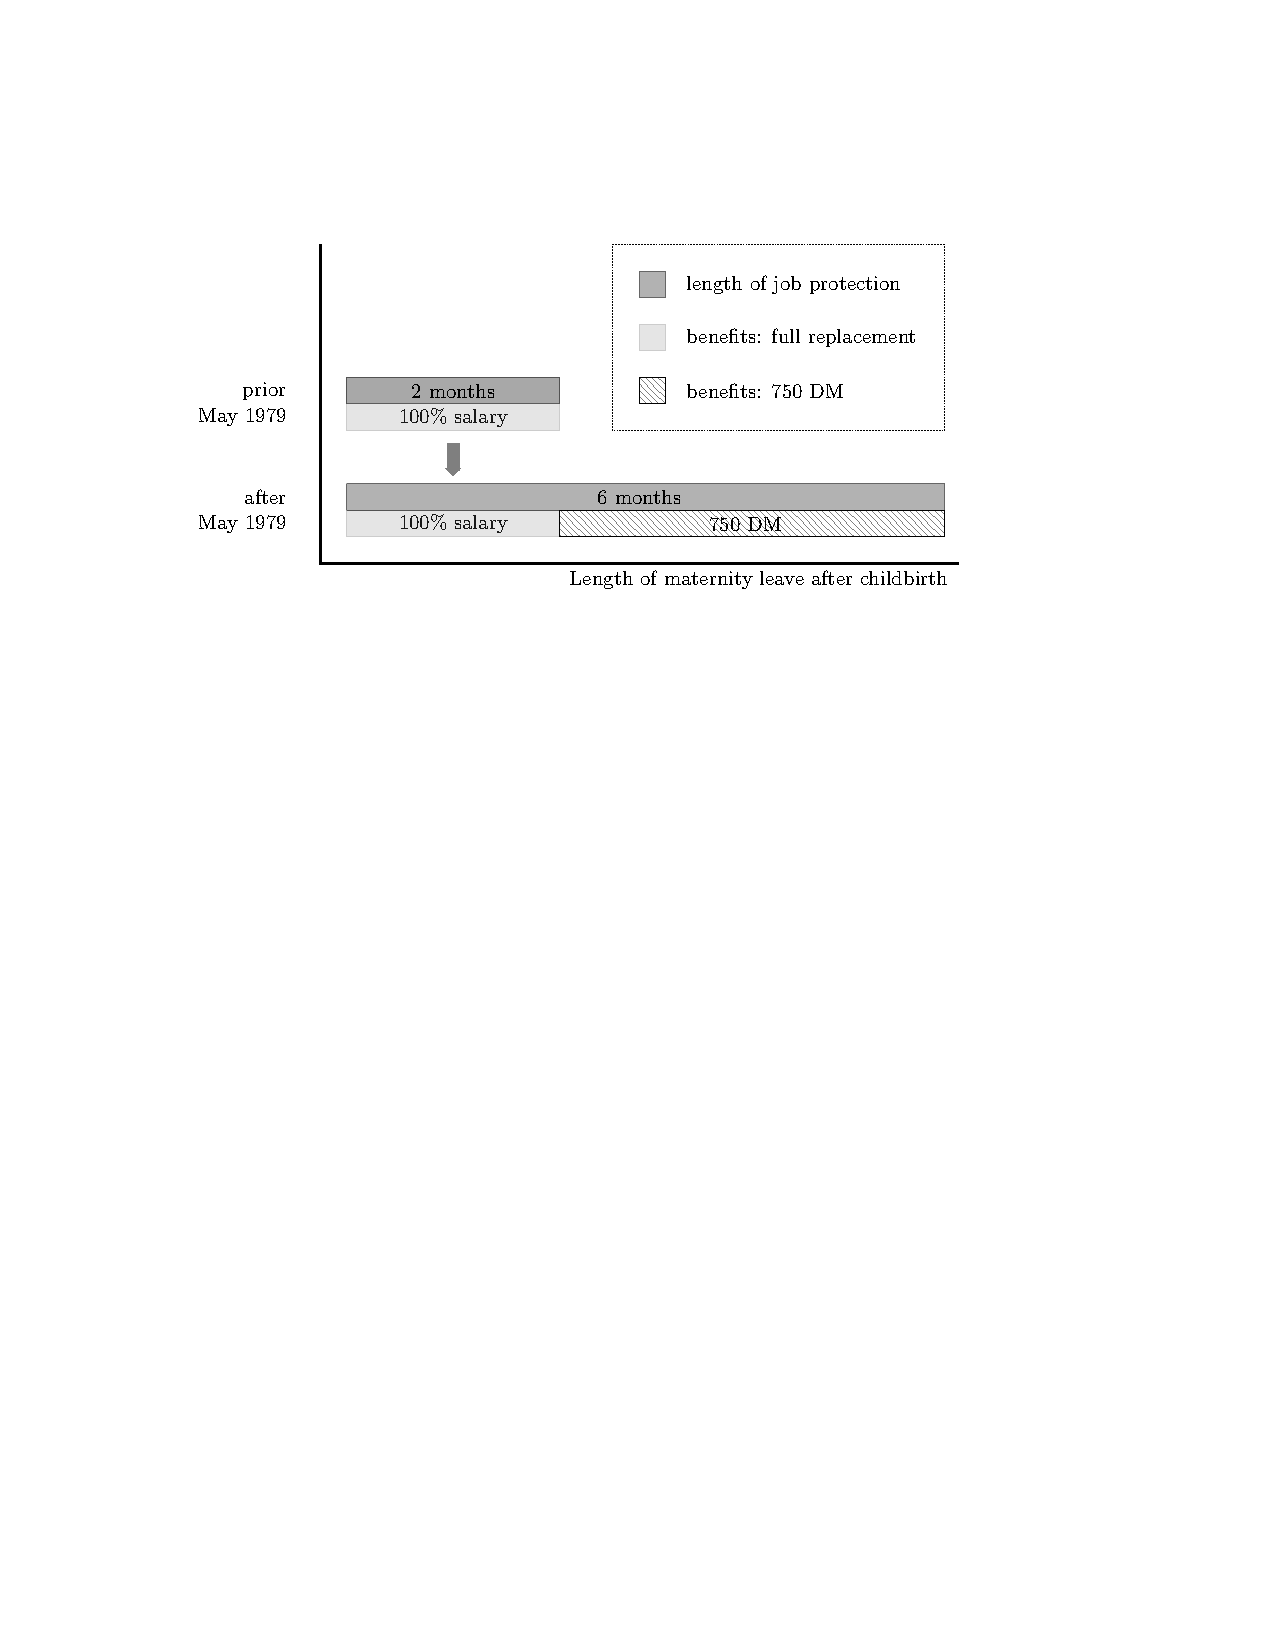
\includegraphics[width=0.8\linewidth]{SOEP/Reform_shortened.pdf}
	\begin{minipage}{\linewidth}
		\scriptsize{\emph{Notes:} The figure describes the legislative change in the length of job protection and ML, which took place in the Federal Republic of Germany in 1979. The reform increased post-birth ML from eight weeks to six months, while keeping the initial structure of the period from six weeks before until eight weeks after childbirth unchanged (mother protection period).\newline \textit{Source: }The figure is based on information from \cite{Dustmann2012}, \cite{DIW2002}, \cite{schonberg2014expansions} as well as \cite{zmarzlik1999mutterschutzgesetz}.}
	\end{minipage}
\end{figure}
%--------------------------------------------
%WMWMWMWMWMWMWMWMWMWMWMWMWMWMWMWMWMWMWMWM
% DATA
%WMWMWMWMWMWMWMWMWMWMWMWMWMWMWMWMWMWMWMWM
%figure TOP 5 Diagnoses across age groups
\vspace*{\fill}
\begin{figure}[H]\centering
	\caption{Five main diagnoses of inpatients aged 0 to 35 in 2014}\label{fig: top5diagnosis_in_2014_across_agegroups}
	\includegraphics[width=0.8\linewidth]{paper/top5diagnoses_across_agegroups.pdf}
	\begin{minipage}{\linewidth}
		\scriptsize{\emph{Notes:} The figure shows the incidence distribution across different age brackets of the top five diagnoses for inpatients aged 0 to 35 in 2014. Diagnoses associated with pregnancy, childbirth, and the puerperium are not taken into account in this representation. The large remainder in the age bracket `0-5' consists mostly of conditions that originate in the perinatal period.}
	\end{minipage}
\end{figure}
\vspace*{\fill}\clearpage
%--------------------------------------------
% figure: matrix descriptive hospital admission
\newpage
\vspace*{\fill}
\begin{figure}[H]\centering
	\caption{Hospital admissions}\label{fig: descriptive_hospital_admission}
	\includegraphics[width=\linewidth]{paper/descriptive_admission_TCG.pdf}
	\begin{minipage}{\linewidth}
		\scriptsize{\emph{Notes:} The figure depicts the evolution of key variables for the treatment and control cohort (only pre-threshold months, i.e. for individuals born between November 1977 and April 1978 as well as November 1978 and April 1979) over the period from 1996 to 2014. The dark lines correspond to the treatment cohorts, whereas control units are marked by light dashed lines. Hospital admissions are defined as the sum of all diagnosis chapters listed in Panel A of Table \ref{tab:outcomes_coding_main_chapters}. This excludes diagnoses of the `O' chapter (pregnancy, childbirth, and the puerperium), among others that occur very infrequently. The x-axis shows in addition to the year the age of the treatment cohort in brackets.} 
	\end{minipage}
\end{figure}
\vspace*{\fill}\clearpage
%--------------------------------------------



%WMWMWMWMWMWMWMWMWMWMWMWMWMWMWMWMWMWMWMWM
% VALIDITY
%WMWMWMWMWMWMWMWMWMWMWMWMWMWMWMWMWMWMWMWM

%--------------------------------------------
% Fertility distribuition
	\vspace*{\fill}
\begin{figure}[H]\centering
	\caption{Daily number of births around the ML expansion}\label{fig: fertilitydistr}
	\includegraphics[width=0.9\linewidth]{paper/fertility_raw_regression_adjusted.pdf}
	\scriptsize
	\begin{minipage}{0.9 \linewidth}
		\emph{Notes:} The figure plots the number of births around the cutoff date May 01, 1979 for the ML expansion from two to six months after childbirth. Panel A shows the raw data, i.e. the actual number of births per day (unadjusted). Panel B, however, plots the difference between the raw and expected number of births when accounting for day of year, public holiday, and year$\times$day of week fixed effects. For the expected number of births I use data in the same time window (one month before and after the threshold) for the years 1977-1990, except for the year in which the reform took place. \newline\emph{Source:} Birth registry data from North Rhine-Westphalia and Baden-Württemberg. Taken together, both states account for almost 36\% of all births in the former Federal Republic of Germany in 1979.
		% {\color{red}how do I get the gray shading from the original figure in the bottom part?}
	\end{minipage}
\end{figure}
\vspace*{\fill}\clearpage





%WMWMWMWMWMWMWMWMWMWMWMWMWMWMWMWMWMWMWMWM
% RESULTS
%WMWMWMWMWMWMWMWMWMWMWMWMWMWMWMWMWMWMWMWM
%--------------------------------------------
\newpage
%Life-course Hospital admission
\begin{landscape}
	\vspace*{\fill}
	\begin{figure}[H]\centering
		\caption{Life-course approach for \textbf{hospital admission}}\label{fig: lc_hospital2_frg_DD}
		\begin{subfigure}[h]{0.31\linewidth}\centering\caption{Total}
			\includegraphics[width=\linewidth]{paper/lc_hospital2_total_gdr.pdf}
		\end{subfigure}
		\begin{subfigure}[h]{0.31\linewidth}\centering\caption{Women}
			\includegraphics[width=\linewidth]{paper/lc_hospital2_female_gdr.pdf}
		\end{subfigure}
		\begin{subfigure}[h]{0.31\linewidth}\centering\caption{Men}
			\includegraphics[width=\linewidth]{paper/lc_hospital2_male_gdr.pdf}
		\end{subfigure}
		\scriptsize
		\begin{minipage}{\linewidth}
			\emph{Notes:} The figures plot DiD estimates (along with 90\% and 95\% confidence intervals) for the impact of the reform on hospital admission over the life-course. The light gray line in the background represents the baseline mean of the pre-reform treated cohort. The outcomes are defined as the number of cases per 1,000 individuals (births). Panel a shows the results for all admissions, whereas panel b and c show the estimates for females and males respectively. The control group is comprised of children	that are born in the same months but one year before the reform (i.e. children born between November 1977 and October 1978).
		\end{minipage}
	\end{figure}
	\vspace*{\fill}\clearpage
\end{landscape}
%--------------------------------------------
% HOPSITAL2 - RD plots
%
% Hospital - Reduced form pooled
\newgeometry{left=1cm,right=1cm,top=3cm,bottom=3cm} 
\begin{landscape}
	\vspace*{\fill}
	\begin{figure}
		[H]\centering
		\caption{RD plots for hospital admission (pooled)}\label{fig: rf_hospital2_pooled}
		\begin{subfigure}[h]{0.31\linewidth}\centering\caption{Total}
			\includegraphics[width=\linewidth]{paper/rd_hospital2_total_pooled.pdf}
		\end{subfigure}
		\begin{subfigure}[h]{0.31\linewidth}\centering\caption{Women}
			\includegraphics[width=\linewidth]{paper/rd_hospital2_female_pooled.pdf}
		\end{subfigure}
		\begin{subfigure}[h]{0.31\linewidth}\centering\caption{Men}
			\includegraphics[width=\linewidth]{paper/rd_hospital2_male_pooled.pdf}
		\end{subfigure}
		\scriptsize
		\begin{minipage}{0.95\linewidth}
			\emph{Notes:} The figure plots the average number of diagnoses per 1,000 individuals for month-of-birth cohorts born half a year around the cut-off date of the 1979 maternity leave expansion. The monthly averages are taken over the entire sample length from 1995 to 2014. The dashed lines represent linear fitted values along with 90\%/95\% confidence intervals. The solid vertical red line divides pre- and post-reform schemes (two vs. six months of leave).\newline
			\emph{Source:} Hospital registry data for individuals born between November 1978 and October 1979.
		\end{minipage}
	\end{figure}
	\vspace*{\fill}\clearpage
\end{landscape}
\restoregeometry  
%--------------------------------------------
% Hospital -Reduced form AGE groups 
% original 3 3 2 3
\newgeometry{left=1cm,right=1cm,top=3cm,bottom=3cm} 
\begin{landscape}
	\vspace*{\fill}
	\begin{figure}
		[H]\centering
		\caption{RD plots for hospital admission across age groups}\label{fig: rf_hospital2_agegroup}
		\includegraphics[width=0.85\linewidth]{paper/rd_r_fert_hospital2_overview_agegroups_CIfits.pdf}
		\scriptsize
		\begin{minipage}{0.9\linewidth}
			\emph{Notes:} The figure plots the number of diagnoses per 1,000 individuals for month-of-birth cohorts born half a year around the cut-off date of the 1979 maternity leave expansion across gender and different age groups. The first column reports the ratios for all patients, and the second and third column do so for women and men, respectively. The rows show the ratios across different age groups. The dashed lines represent linear fitted values along with 90\%/95\% confidence intervals. The solid vertical red line divides pre- and post-reform schemes (two vs. six months of leave).\newline
			\emph{Source:} Hospital registry data for individuals born between November 1978 and October 1979.
		\end{minipage}
	\end{figure}
	\vspace*{\fill}\clearpage
\end{landscape}
\restoregeometry

%--------------------------------------------
% Figure: effect sizes and frequency across chapters

\begin{landscape}
	\vspace*{\fill}
	\begin{figure}[H]\centering
		\caption{Intention-to-treat effects across \textbf{main diagnosis chapters}}\label{fig: DD_across_main chapters}
		\begin{subfigure}[h]{0.31\linewidth}\centering\caption{Total}
			\includegraphics[width=\linewidth]{paper/effect_chapters_frequency.pdf}
		\end{subfigure}
		\begin{subfigure}[h]{0.31\linewidth}\centering\caption{Women}
			\includegraphics[width=\linewidth]{paper/effect_chapters_frequency_f.pdf}
		\end{subfigure}
		\begin{subfigure}[h]{0.31\linewidth}\centering\caption{Men}
			\includegraphics[width=\linewidth]{paper/effect_chapters_frequency_m.pdf}
		\end{subfigure}
		\scriptsize
		\begin{minipage}{\linewidth}
			\emph{Notes:} The figures plots intention-to-treat estimates (along with 90\%/95\% confidence intervals) across the main diagnosis chapters. Furthermore, they indicate how often each chapter is diagnosed over the entire time frame (1995-2014). The outcomes are defined as the number of cases per 1,000 individuals (births). The point estimates are coming from a DiD regression as described in section \ref{sec:empirical_strategy}, with a bandwidth of six months, month-of-birth and year fixed effects, and clustered standard errors on the month-of-birth level. The control group is comprised of children	that are born in the same months but one year before the reform (i.e. children born between November 1977 and October 1978). \newline
			\emph{Legend:} Infectious and parasitic diseases (IPD), neoplasms (Neo), mental and behavioral disorders (MBD), diseases of the nervous system (Ner), diseases of the sense organs (Sen), diseases of the circulatory system (Cir), diseases of the respiratory system (Res), diseases of the digestive system (Dig), diseases of the skin and subcutaneous tissue (SST), diseases of the musculoskeletal system (Mus), diseases of the genitourinary system (Gen), symptoms, signs, and ill-defined conditions (Sym), injury, poisoning and certain other consequences of external causes (Ext).
			
		\end{minipage}
	\end{figure}
	\vspace*{\fill}\clearpage
\end{landscape}
%--------------------------------------------

% D5 - LC Approach (Mental and behavioral disod)
\begin{landscape}
	\vspace*{\fill}
	\begin{figure}[H]\centering
		\caption{Life-course approach for \textbf{mental and behavioral disorders}}\label{fig: lc_d5_frg_DD}
		\begin{subfigure}[h]{0.31\linewidth}\centering\caption{Total}
			\includegraphics[width=\linewidth]{paper/lc_d5_total_gdr.pdf}
		\end{subfigure}
		\begin{subfigure}[h]{0.31\linewidth}\centering\caption{Women}
			\includegraphics[width=\linewidth]{paper/lc_d5_female_gdr.pdf}
		\end{subfigure}
		\quad
		\begin{subfigure}[h]{0.31\linewidth}\centering\caption{Men}
			\includegraphics[width=\linewidth]{paper/lc_d5_male_gdr.pdf}
		\end{subfigure}
		\scriptsize
		\begin{minipage}{\linewidth}
			\emph{Notes:} The figures plot DiD estimates (along with 90\% and 95\% confidence intervals) for the impact of the reform on mental and behavioral disorders over the life-course. The light gray line in the background represents the baseline mean of the pre-reform treated cohort. The outcomes are defined as the number of cases per 1,000 individuals (births). Panel a shows the results for all admissions, whereas panel b and c show the estimates for females and males respectively. The control group is comprised of children	that are born in the same months but one year before (i.e. children born between November 1977 and October 1978).
		\end{minipage}
	\end{figure}
	\vspace*{\fill}\clearpage
\end{landscape}

%--------------------------------------------
% D5 RD plots
%
% d5 - RF pooled
\newgeometry{left=1cm,right=1cm,top=3cm,bottom=3cm} 
\begin{landscape}
	\vspace*{\fill}
	\begin{figure}
		[H]\centering
		\caption{RD plots for mental \& behavioral disorders (pooled)}\label{fig: rf_d5_pooled}
		\begin{subfigure}[h]{0.31\linewidth}\centering\caption{Total}
			\includegraphics[width=\linewidth]{paper/rd_d5_total_pooled.pdf}
		\end{subfigure}
		\begin{subfigure}[h]{0.31\linewidth}\centering\caption{Women}
			\includegraphics[width=\linewidth]{paper/rd_d5_female_pooled.pdf}
		\end{subfigure}
		\begin{subfigure}[h]{0.31\linewidth}\centering\caption{Men}
			\includegraphics[width=\linewidth]{paper/rd_d5_male_pooled.pdf}
		\end{subfigure}
		\scriptsize
		\begin{minipage}{0.95\linewidth}
			\emph{Notes:} The figure plots the average number of diagnoses per 1,000 individuals for month-of-birth cohorts born half a year around the cut-off date of the 1979 maternity leave expansion. The monthly averages are taken over the entire sample length from 1995 to 2014. The dashed lines represent linear fitted values along with 90\%/95\% confidence intervals. The solid vertical red line divides pre- and post-reform schemes (two vs. six months of leave).\newline
			\emph{Source:} Hospital registry data for individuals born between November 1978 and October 1979.
		\end{minipage}
	\end{figure}
	\vspace*{\fill}\clearpage
\end{landscape}
\restoregeometry 




%--------------------------------------------
% D5 - RF (age group)
\newgeometry{left=1cm,right=1cm,top=3cm,bottom=3cm} 
\begin{landscape}
	\vspace*{\fill}
	\begin{figure}
		[H]\centering
		\caption{RD plots for mental \& behavioral disorders across age groups}\label{fig: rf_d5_agegroup}
		\includegraphics[width=0.85\linewidth]{paper/rd_r_fert_d5_overview_agegroups_CIfits.pdf}
		\scriptsize
		\begin{minipage}{0.9\linewidth}
			\emph{Notes:} The figure plots the number of diagnoses per 1,000 individuals for month-of-birth cohorts born half a year around the cut-off date of the 1979 maternity leave expansion across gender and different age groups. The first column reports the ratios for all patients, and the second and third column do so for women and men, respectively. The rows show the ratios across different age groups. The dashed lines represent linear fitted values along with 90\%/95\% confidence intervals. The solid vertical red line divides pre- and post-reform schemes (two vs. six months of leave).\newline
			\emph{Source:} Hospital registry data for individuals born between November 1978 and October 1979.
		\end{minipage}
	\end{figure}
	\vspace*{\fill}\clearpage
\end{landscape}
\restoregeometry

 
%--------------------------------------------
% Graph D5 partition - Subcategories
\vspace*{\fill}
\begin{figure}[H]\centering
	\caption{The top five subcategories of mental and behavioral diagnoses}\label{fig: d5partition}
	\includegraphics[width=0.8\linewidth]{../../analysis/graphs/paper/d5partition_lfstat.pdf}
	\scriptsize
	\begin{minipage}{0.9\linewidth}
	\emph{Notes:} This figure plots the yearly number of diagnoses for the treatment cohort (i.e. the individuals born between November 1978 and October 1979). The subcategories are ordered by their occurrence in 2014 (from the most to the least frequent diagnosis), which also coincides by chance with the ordering in the ICD-10 classification system. The five most frequent subcategories - as shown here - comprise more than 95\% of all MBDs. 
	\end{minipage}
\end{figure}
\vspace*{\fill}\clearpage%--------------------------------------------
% figure: iverview of d5 subcategories (effects + frequency)
\newgeometry{left=1cm,right=1cm,top=3cm,bottom=3cm} 
\begin{landscape}
	\vspace*{\fill}
	\begin{figure}
		[H]\centering
		\caption{ITT effect for \textbf{subcategories of mental and behavioral disorders (pooled)}}\label{fig: ITT_d5_subcategories}
		\begin{subfigure}[h]{0.31\linewidth}\centering\caption{Total}
			\includegraphics[width=\linewidth]{paper/effect_d5_frequency.pdf}
		\end{subfigure}
		\begin{subfigure}[h]{0.31\linewidth}\centering\caption{Women}
			\includegraphics[width=\linewidth]{paper/effect_d5_frequency_f.pdf}
		\end{subfigure}
		\begin{subfigure}[h]{0.31\linewidth}\centering\caption{Men}
			\includegraphics[width=\linewidth]{paper/effect_d5_frequency_m.pdf}
		\end{subfigure}
		\scriptsize
		\begin{minipage}{0.95\linewidth}
			\emph{Notes:} The figure plots ITT estimates (along with 90\%/95\% confidence intervals) across the five most common subcategories of MBDs. Moreover, they indicate how often each subcategory is diagnosed over the time window of 1995-2014. The outcomes are defined as the number of cases per 1,000 individuals (births). The point estimates are coming from a DiD regression as described in section \ref{sec:empirical_strategy}, with a bandwidth of six months, month-of-birth and year fixed effects, and standard errors clustered at the month-of-birth level. The control group is comprised of children that are born in the same months but one year before the reform (i.e. children born between November 1977 and October 1978).\newline
			\emph{Source:} Hospital registry data.
		\end{minipage}
	\end{figure}
	\vspace*{\fill}\clearpage
\end{landscape}
\restoregeometry 






%--------------------------------------------------------------------
% TABLES
%--------------------------------------------------------------------
\newpage
\TODO\section{Tables}
\vspace*{\fill}
{\Huge \begin{center}\textbf{TABLES}\end{center}}
\vspace*{\fill}\clearpage

%--------------------------------------------
% Overview ICD 9 and ICD 10 
%\begin{small}
%\vspace*{\fill}
%\begin{table}[h] % table environment for caption and label
%	\begin{threeparttable}
%		\centering % center the tabular
%		\caption{Overview of diagnoses} % caption
%		\label{tab:outcomes_coding_main_chapters} 
%		\begin{tabular}{lrrr} % alignment and number of columns of actual table
%			\toprule % top thicker horizontal line (" rule ")
%			&\multicolumn{1}{r}{(1)}& &\multicolumn{1}{r}{(2)}\\
%			&\multicolumn{1}{r}{ICD-9} & & \multicolumn{1}{r}{ICD-10} \\ 
%			\midrule
%			%-------------------------------------------------------------------------
%			\textit{Main diagnosis chapters}\\
 \hspace{4pt} Infectious and parasitic diseases                           	&	001-139		& &		A00-B99 \\
 \hspace{4pt} Neoplasms                                                   	&	140-239		& &		C00-D48 \\
%\hspace{4pt} Diseases of the blood and blood-forming organs              	&	280-289		& &		D50-D90 \\
 \hspace{4pt} Endocrine, nutritional and metabolic diseases					&	240-278		& &		E00-E90 \\
 \hspace{4pt} Mental \& behavioral  disorders                             	&	290-319		& &		F00-F99 \\
 \hspace{4pt} Diseases of the nervous system                              	&	320-359		& &		G00-G99 \\
 \hspace{4pt} Diseases of the sense organs                                	&	360-389		& &		H00-H95 \\
 \hspace{4pt} Diseases of the circulatory system                          	&	390-459		& &		I00-I99 \\
 \hspace{4pt} Diseases of the respiratory system                          	&	460-519		& &		J00-J99 \\
 \hspace{4pt} Diseases of the digestive system                            	&	520-579		& &		K00-K93 \\
 \hspace{4pt} Diseases of the skin and subcutaneous tissue                	&	680-709		& &		L00-L99 \\
 \hspace{4pt} Diseases of the musculoskeletal system and connective tissue	&	710-739		& &		M00-M99 \\
 \hspace{4pt} Diseases of the genitourinary system                        	&	580-629		& &		N00-N99 \\
 \hspace{4pt} Complications of pregnancy, childbirth, and the puerperium  	&	630-676		& &		O00-O99 \\
%\hspace{4pt} Certain conditions originating in the perinatal period      	&	760-779		& &		P00-P96 \\
%\hspace{4pt} Congenital anomalies                                        	&	740-759		& &		Q00-Q99 \\
 \hspace{4pt} Symptoms, signs, and ill-defined conditions                 	&	780-799		& &		R00-R99 \\
 \hspace{4pt} Injury and poisoning                                        	&	800-999		& &		S00-T98 \\
 \\
 \textit{}

\
%			%-------------------------------------------------------------------------
%			\bottomrule % bottom thicker horizontal line (" rule ")
%		\end{tabular}
%		\begin{tablenotes}
%			\scriptsize{ \item \textit{Notes:} The table shows the classification of diseases according to the "International Statistical Classification of Diseases and Related Health Problems (ICD)", a medical classification list provided by the World Health Organization. \newline \textit{Source:} World Health Organization (WHO), see for example: \href{http://www.who.int/classifications/icd/en/}{http://www.who.int/classifications/icd/en/}\newline$^1$ Psychoactive substances include alcohol, opioids, cannabinoids, sedatives or hypnotics, cocaine, other stimulants (including caffeine), hallucinogens, tobacco, volatile solvents, multiple drug use and use of other psychoactive substances. }
%		\end{tablenotes}
%	\end{threeparttable}
%\end{table}
%\vspace*{\fill}\clearpage 
%%\end{small}
%%\normalsize


%--------------------------------------------
% Overview Hopsital admission
\newgeometry{left=0cm,right=0cm,top=0cm,bottom=3cm} 

\begin{landscape}
	\vspace*{\fill}
	\begin{table}[h] \centering % table environment for caption and label
		\begin{threeparttable}
			\centering % center the tabular
			\caption{Summary statistics for different diagnoses} % caption
			\label{tab:outcomes_coding_main_chapters} 
			\begin{tabular}{lrrrrrr} % alignment and number of columns of actual table
				\toprule % top thicker horizontal line (" rule ")
				&\multicolumn{1}{r}{(1)}& &\multicolumn{1}{r}{(2)}&\multicolumn{1}{r}{(3)} &\multicolumn{1}{r}{(4)}\\
				&\multicolumn{1}{r}{ICD-9} & & \multicolumn{1}{r}{ICD-10}&\multicolumn{1}{r}{Mean}&\multicolumn{1}{r}{SD} \\ 
				\midrule
				%-------------------------------------------------------------------------
				\\
\underline{\textit{A. Hospital admission}}									& 						& & 			 & 	 120.625     &  10.961\\ 
 \hspace{10pt} Infectious and parasitic diseases                           	&	001-139				& &		A00-B99  & 	   4.210     &   0.493\\
 \hspace{10pt} Neoplasms                                                   	&	140-239				& &		C00-D48  & 	   5.155     &   1.282\\
 \hspace{10pt} Mental \& behavioral  disorders                             	&	290-319				& &		F00-F99  & 	  18.956     &   5.548\\
 \hspace{10pt} Diseases of the nervous system                              	&	320-359				& &		G00-G99  & 	   4.500     &   1.264\\
 \hspace{10pt} Diseases of the sense organs                                	&	360-389				& &		H00-H95  & 	   2.404     &   0.348\\
 \hspace{10pt} Diseases of the circulatory system                          	&	390-459				& &		I00-I99  & 	   4.108     &   1.380\\
 \hspace{10pt} Diseases of the respiratory system                          	&	460-519				& &		J00-J99  & 	  10.994     &   1.939\\
 \hspace{10pt} Diseases of the digestive system                            	&	520-579				& &		K00-K93  & 	  16.746     &   2.079\\
 \hspace{10pt} Diseases of the skin and subcutaneous tissue                	&	680-709				& &		L00-L99  & 	   3.849     &   0.536\\
 \hspace{10pt} Diseases of the musculoskeletal system						&	710-739				& &		M00-M99  & 	   8.897     &   2.228\\
 \hspace{10pt} Diseases of the genitourinary system                        	&	580-629				& &		N00-N99  & 	  10.621     &   1.362\\
 \hspace{10pt} Symptoms, signs, and ill-defined conditions                 	&	780-799				& &		R00-R99  & 	   6.794     &   1.410\\
 \hspace{10pt} Injury, poisoning and certain other                          &	800-999				& &		S00-T98  & 	  21.196     &   5.978\\
 \hspace{18pt} consequences of external causes  \\
 
 %\hspace{4pt} Diseases of the blood and blood-forming organs              	&	280-289		& &		D50-D90  & \\
 %\hspace{4pt} Endocrine, nutritional and metabolic diseases				&	240-278		& &		E00-E90  & \\
 %\hspace{4pt} Pregnancy, childbirth, and the puerperium  					&	630-676		& &		O00-O99  & \\
 %\hspace{4pt} Certain conditions originating in the perinatal period      	&	760-779		& &		P00-P96  & \\
 %\hspace{4pt} Congenital anomalies                                        	&	740-759		& &		Q00-Q99  & \\
 
 
 % ------------------------------------------------------------------------
 % 							Mean           SD          Min          Max
 % ------------------------------------------------------------------------
 % Ratio using number~e      120.625       10.961        99.27       156.35
 % Ratio using number~e        4.210        0.493         2.87         5.65
 % Ratio using number~e        5.155        1.282         3.29         8.97
 % Ratio using number~e       18.956        5.548         6.68        30.17
 % Ratio using number~e        4.500        1.264         2.60         7.50
 % Ratio using number~e        2.404        0.348         1.62         3.07
 % Ratio using number~e        4.108        1.380         1.41         7.66
 % Ratio using number~e       10.994        1.939         8.30        15.55
 % Ratio using number~e       16.746        2.079        12.09        20.97
 % Ratio using number~e        3.849        0.536         2.63         5.12
 % Ratio using number~e        8.897        2.228         6.45        15.46
 % Ratio using number~e       10.621        1.362         6.79        13.64
 % Ratio using number~e        6.794        1.410         4.26        10.70
 % Ratio using number~e       21.196        5.978        14.41        34.06
 % ------------------------------------------------------------------------



				%-------------------------------------------------------------------------
				\bottomrule % bottom thicker horizontal line (" rule ")
			\end{tabular}
			\begin{tablenotes}
				\scriptsize{ \item \textit{Continued on next page}}
			\end{tablenotes}
		\end{threeparttable}
	\end{table}
	\vspace*{\fill}\clearpage 
	
	
	\vspace*{\fill}
	\begin{table}[h] \centering % table environment for caption and label
		\begin{threeparttable}
			\centering % center the tabular
			\caption*{\textit{Summary statistics for different diagnoses (continued)}} % caption

			\begin{tabular}{lrrrrrr} % alignment and number of columns of actual table
				\toprule % top thicker horizontal line (" rule ")
				&\multicolumn{1}{r}{(1)}& &\multicolumn{1}{r}{(2)}&\multicolumn{1}{r}{(3)} &\multicolumn{1}{r}{(4)}\\
				&\multicolumn{1}{r}{ICD-9} & & \multicolumn{1}{r}{ICD-10}&\multicolumn{1}{r}{Mean}&\multicolumn{1}{r}{SD} \\ 
				\midrule
				%-------------------------------------------------------------------------
				

\\
\underline{\textit{B. Mental \& behavioral disorders}}						&						& & 			 & 18.956		& 5.548		\\
 \hspace{10pt} Organic, including symptomatic, mental disorders				& 290,293,294,310		& & 	F00-F09	 &	0.115		& 0.056		\\
 \hspace{10pt} MBD due to psychoactive substance use$^1$					& 291,292,303,304,305	& & 	F10-F19	 &	6.366		& 2.232		\\
 \hspace{10pt} Schizophrenia, schizotypal and delusional disorders			& 295,297,298			& & 	F20-F29	 &	5.140		& 2.246		\\
 \hspace{10pt} Mood [affective] disorders									& 296,311				& & 	F30-F39	 &	2.339		& 1.673		\\
 \hspace{10pt} Neurotic, stress-related and somatoform disorders			& 300,306,308,309		& & 	F40-F48	 &	2.799		& 0.356		\\
 \hspace{10pt} Behavioural syndromes associated with 						& 316					& & 	F50-F59	 &	0.308		& 0.225		\\
 \hspace{18pt} physiological disturbances and physical factors 														 &				& 			\\
 \hspace{10pt} Disorders of adult personality and behavior					& 301,302				& & 	F60-F69	 &	1.375		& 0.511		\\
 \hspace{10pt} Mental retardation 											& 317,318,319			& &		F70-F79	 &	0.121		& 0.075		\\
 \hspace{10pt} Disorders of psychological development						& 299,315				& & 	F80-F89	 &	0.026		& 0.029		\\
 \hspace{10pt} Behavioural and emotional disorders with 					& 312,313,314,307		& & 	F90-F98	 &	0.320		& 0.535		\\
  \hspace{18pt} onset usually occurring in childhood and adolescence 																			\\


% var			mean	SD
% d5						18.956	5.548
% organic					0.115	0.056
% psychoactive substances	6.366	2.232
% schizophrenia			5.140	2.246
% affective				2.339	1.673
% neurosis				2.799	0.356
% physical factors		0.308	0.225
% personality				1.375	0.511
% retardation				0.121	0.075
% development				0.026	0.029
% childhood				0.320	0.535
		


				%-------------------------------------------------------------------------
				\bottomrule % bottom thicker horizontal line (" rule ")
			\end{tabular}
			\begin{tablenotes}
				\scriptsize{ \item \textit{Notes:} The table shows the classification of diseases according to the `International Statistical Classification of Diseases and Related Health Problems (ICD)', a medical classification list provided by the World Health Organization. For the main chapters, the mapping between ICD-9 and ICD-10 is taken from the European shortlist. The table reports next to the ICD codes summary statistics for the different diagnosis types. Column 3 and 4 show mean and standard deviation of the number of diagnoses per 1,000 individuals for the pre-reform treatment cohort. The data uses the modified version of the ICD system issued by DIMDI.\newline \textit{Source:} The ICD coding is taken from the World Health Organization (WHO), see for example: \href{http://www.who.int/classifications/icd/en/}{http://www.who.int/classifications/icd/en/} and the European shortlist \citep[p. 76]{statistisches2012diagnosedaten}, the summary statistics are obtained from the hospital registry data. \newline\hspace*{15 pt}$^1$ Psychoactive substances include alcohol, opioids, cannabinoids, sedatives or hypnotics, cocaine, other stimulants (including caffeine), hallucinogens, tobacco, volatile solvents, multiple drug use and use of other psychoactive substances. }
			\end{tablenotes}
		\end{threeparttable}
	\end{table}
	\vspace*{\fill}\clearpage 
\end{landscape}
\restoregeometry
%--------------------------------------------
%VALIDITY: Birth rate effects
 \vspace*{\fill}
 \begin{table}[H] \centering
 \caption{Birth rate effects of the 1979 ML reform}\label{tab: validity_birth_rate}
 {\def\sym#1{\ifmmode^{#1}\else\(^{#1}\)\fi} 
 \begin{tabular}{l*{5}{c}}
 	\toprule
 	& \multicolumn{4}{c}{Estimation window} \\
 	\cmidrule{2-5}
 	&\multicolumn{1}{c}{(1)}&\multicolumn{1}{c}{(2)}&\multicolumn{1}{c}{(3)}&\multicolumn{1}{c}{(4)}\\
	 & \multicolumn{1}{c}{$\pm$7 days} & \multicolumn{1}{c}{$\pm$14 days} & \multicolumn{1}{c}{$\pm$21 days} & \multicolumn{1}{c}{$\pm$28 days}\\ 
 	\midrule
 	\multicolumn{5}{l}{\emph{Panel A. Dependent variable is number of births}}\\
 	ML reform           &      -30.46         &      -30.23\sym{*}  &      -33.32\sym{**} &      -32.78\sym{***}\\
                    &     (30.31)         &     (17.73)         &     (14.08)         &     (12.37)         \\
Observations        &         196         &         392         &         588         &         784         \\
$R^2$               &       0.856         &       0.842         &       0.832         &       0.817         \\

 	\\ \\
 	\multicolumn{5}{l}{\emph{Panel B. Dependent variable is ln(number of births)}}\\
 	ML reform           &     -0.0448         &     -0.0440\sym{*}  &     -0.0477\sym{**} &     -0.0476\sym{***}\\
                    &    (0.0425)         &    (0.0247)         &    (0.0197)         &    (0.0173)         \\
Observations        &         196         &         392         &         588         &         784         \\
$R^2$               &       0.855         &       0.844         &       0.833         &       0.819         \\

 	\bottomrule
 \end{tabular}}
 \begin{minipage}{0.7\linewidth}
 		\scriptsize \emph{Notes:} The table shows regression estimates of the impact of the 1979 ML reform on fertility. The sample comprises daily births within the relevant estimation window in the federal states of Baden-Württemberg and North Rhine-Westphalia from 1977-1990. Panel A uses the number of births as dependent variable, whereas panel B shows results with the log of the number of births as dependent variable. All specifications control for day of year, public holiday, and year$\times$day of week fixed effects. The estimation window is referring to the number of days before and after May 01. For instance, the $\pm$ 7 day window includes the last week in April and the first week in May across all years. Standard errors are reported in parentheses. \newline Significance levels: * p < 0.10, ** p < 0.05, *** p < 0.01. \newline\emph{Source:} Birth registry data from North Rhine-Westphalia and Baden-Württemberg. Taken together, both states account for almost 36\% of all births in the former Federal Republic of Germany in 1979.
 	\end{minipage}
 \end{table}
 \vspace*{\fill}\clearpage 

%--------------------------------------------
% HOSPITAL - Difference in Difference tables for 
\newpage

\begin{table}[t] \centering 
 \begin{threeparttable} \centering \caption{ITT effects on hospital admission}\label{tab_mlch: DD_hopsital2_total}
  {\def\sym#1{\ifmmode^{#1}\else\(^{#1}\)\fi} 
 	\begin{tabular}{l*{6}{c}}
 		\toprule 
 		%\multicolumn{5}{l}{Dependant variable: \textbf{Hospital admission (total)}}\\ \\ 
 		& \multicolumn{5}{c}{Estimation window} \\ 
 		\cmidrule(lr){2-6}
 		&\multicolumn{1}{c}{(1)}&\multicolumn{1}{c}{(2)}&\multicolumn{1}{c}{(3)}&\multicolumn{1}{c}{(4)}&\multicolumn{1}{c}{(5)}\\
 		&\multicolumn{1}{c}{6M}&\multicolumn{1}{c}{5M}&\multicolumn{1}{c}{4M}&\multicolumn{1}{c}{3M}&\multicolumn{1}{c}{Donut}\\
 		\midrule
 		\multicolumn{5}{l}{\emph{Panel A. Over entire length of the life-course}} \\
 		\hspace*{10pt}Overall&      -2.218         &      -2.181\sym{*}  &      -1.944\sym{**} &      -2.168\sym{**} &      -2.713\sym{***}\\
                    &     (1.401)         &     (1.143)         &     (0.917)         &     (0.782)         &     (0.826)         \\
\midrule Dependent mean&       122.7         &       121.0         &       120.5         &       120.6         &       121.4         \\
Effect in SDs [\%]  &       19.22         &       18.84         &       17.35         &       19.78         &       24.62         \\
Observations        &         240         &         320         &         400         &         480         &         400         \\
 \\ \\
 		\multicolumn{5}{l}{\emph{Panel B. Age brackets}} \\
 		\hspace*{10pt}Age 17-21&      -1.095         &      -0.735         &      -0.590         &      -1.517\sym{+}  &      -1.963\sym{**} \\
                    &     (1.603)         &     (1.198)         &     (0.995)         &     (0.946)         &     (0.931)         \\
 \hspace*{10pt}Age 22-26&      -0.735         &      -0.667         &      -0.613         &      -0.611         &      -1.080         \\
                    &     (1.672)         &     (1.412)         &     (1.113)         &     (0.937)         &     (1.012)         \\
 \hspace*{10pt}Age 27-31&      -2.546\sym{*}  &      -3.209\sym{**} &      -3.015\sym{***}&      -2.665\sym{***}&      -2.974\sym{***}\\
                    &     (1.375)         &     (1.132)         &     (0.909)         &     (0.826)         &     (0.949)         \\
 \hspace*{10pt}Age 32-35&      -3.869\sym{***}&      -3.619\sym{**} &      -4.572\sym{***}&      -5.045\sym{**} &      -4.717\sym{***}\\
                    &     (1.083)         &     (1.277)         &     (1.460)         &     (1.721)         &     (1.191)         \\
 
 		\bottomrule 
 	\end{tabular}}
 	\begin{tablenotes} 
 		\item \scriptsize \emph{Notes:} The table shows DiD estimates of the 1979 maternity leave reform on hospital admission for different estimation windows around the cutoff. The \textit{`Donut'} specification uses a bandwidth of half a year and excludes children born in April and May. Panel A shows the effect for the entire pooled time frame and panel B reports estimates per age bracket. The outcome variables are defined as the number of cases per thousand individuals. All regressions control for year and month-of-birth fixed effects. The control group is comprised of children that are born in the same months but one year before the reform (i.e. children born between November 1977 and October 1978). In order to compare the two birth cohorts at the same age, I shift the control cohort from wave $t$ to wave $t+1$. The dependent mean and the effect size in standard deviation units correspond to pre-reform values of the treated group. Table \ref{tab_mlch: observations_age_brackets} contains the number of observations for the estimations per age bracket. Clustered standard errors are reported in parentheses. \newline Significance levels: * p < 0.10, ** p < 0.05, *** p < 0.01. \newline 	%\emph{Source:} Hospital registry data.
 	\end{tablenotes} 
 \end{threeparttable} 
 \end{table}
\vspace*{\fill}
 \begin{table}[H] \centering 
 	\begin{threeparttable} \centering \caption{ITT effects on \textbf{hospital admission (women)}}\label{tab: DD_hopsital2_female} {\def\sym#1{\ifmmode^{#1}\else\(^{#1}\)\fi} 
 			\begin{tabular}{l*{6}{c}}
 				\toprule 
 				%\multicolumn{5}{l}{Dependant variable: \textbf{Hospital admission (total)}}\\ \\ 
 				& \multicolumn{5}{c}{Estimation window} \\ 
 				\cmidrule(lr){2-6}
 				&\multicolumn{1}{c}{(1)}&\multicolumn{1}{c}{(2)}&\multicolumn{1}{c}{(3)}&\multicolumn{1}{c}{(4)}&\multicolumn{1}{c}{(5)}\\
 				&\multicolumn{1}{c}{6M}&\multicolumn{1}{c}{5M}&\multicolumn{1}{c}{4M}&\multicolumn{1}{c}{3M}&\multicolumn{1}{c}{Donut}\\
 				\midrule
 				\multicolumn{5}{l}{\emph{Panel A.Over entire length of the life-course}} \\
 				\hspace*{10pt}Overall&       0.149         &      -0.766         &      -1.815\sym{**} &      -2.278\sym{***}\\
                    &     (2.038)         &     (1.088)         &     (0.807)         &     (0.751)         \\
\midrule Dependent mean&       122.3         &       122.0         &       122.4         &       123.3         \\
Effect in SDs [\%]  &       1.350         &       6.530         &       16.29         &       20.28         \\
Observations        &         160         &         320         &         480         &         400         \\
 \\ \\
 				\multicolumn{5}{l}{\emph{Panel B. Age brackets}} \\
 				\hspace*{10pt}Age 17-21&      -2.121\sym{+}  &      -1.274         &      -1.931\sym{*}  &      -2.916\sym{***}&      -3.322\sym{***}\\
                    &     (1.269)         &     (1.018)         &     (0.959)         &     (0.935)         &     (0.985)         \\
 \hspace*{10pt}Age 22-26&       1.661         &       1.126         &      0.0274         &      -0.510         \\
                    &     (3.675)         &     (1.806)         &     (1.267)         &     (1.117)         \\
 \hspace*{10pt}Age 27-31&      -1.379         &      -1.669         &      -2.605\sym{**} &      -2.762\sym{**} &      -2.944\sym{***}\\
                    &     (1.765)         &     (1.336)         &     (1.163)         &     (1.004)         &     (0.917)         \\
 \hspace*{10pt}Age 32-35&      -0.605         &      -1.004         &      -0.841         &      -1.212         &      -1.810\sym{*}  \\
                    &     (1.300)         &     (1.165)         &     (1.024)         &     (0.866)         &     (0.941)         \\
 
 				\bottomrule 
 		\end{tabular}}
 		\begin{tablenotes} 
 			\item \scriptsize \emph{Notes:} The table shows DiD estimates of the 1979 maternity leave reform on hospital admission for different estimation windows around the cutoff. The \textit{`Donut'} specification uses a bandwidth of half a year and excludes children born in April and May. Panel A shows the effect for the entire pooled time frame and panel B breaks the life-course up in age brackets. The outcome variables are defined as the number of cases per thousand individuals (births). All regressions control for year and month-of-birth fixed effects. The control group is comprised of children that are born in the same months but one year before the reform (i.e. children born between November 1977 and October 1978). In order to compare the two birth cohorts at the same age, I shift the control cohort from wave $t$ to wave $t+1$. The dependent mean and the effect size in standard deviation units correspond to pre-reform values of the treated group. Clustered standard errors are reported in parentheses. \newline Significance levels: + p < 0.15, * p < 0.10, ** p < 0.05, *** p < 0.01. \newline 	\emph{Source:} Hospital registry data.
 		\end{tablenotes} 
 	\end{threeparttable} 
 \end{table}
\vspace*{\fill}\clearpage 
 \vspace*{\fill}
 \begin{table}[H] \centering 
 	\begin{threeparttable} \centering \caption{ITT effects on \textbf{hospital admission (men)}}\label{tab: DD_hopsital2_male} {\def\sym#1{\ifmmode^{#1}\else\(^{#1}\)\fi} 
 		\begin{tabular}{l*{6}{c}}
 			\toprule 
 			%\multicolumn{5}{l}{Dependant variable: \textbf{Hospital admission (total)}}\\ \\ 
 			& \multicolumn{5}{c}{Estimation window} \\ 
 			\cmidrule(lr){2-6}
 			&\multicolumn{1}{c}{(1)}&\multicolumn{1}{c}{(2)}&\multicolumn{1}{c}{(3)}&\multicolumn{1}{c}{(4)}&\multicolumn{1}{c}{(5)}\\
 			&\multicolumn{1}{c}{6M}&\multicolumn{1}{c}{5M}&\multicolumn{1}{c}{4M}&\multicolumn{1}{c}{3M}&\multicolumn{1}{c}{Donut}\\
 				\midrule
 				\multicolumn{5}{l}{\emph{Panel A. Over entire length of the life-course}} \\
 				\hspace*{10pt}Overall&      -0.445         &      -3.528\sym{**} &      -2.525\sym{**} &      -3.148\sym{**} \\
                    &     (1.017)         &     (1.387)         &     (0.997)         &     (1.144)         \\
\midrule Dependent mean&       118.3         &       120.0         &       118.9         &       119.7         \\
Effect in SDs [\%]  &       3.440         &       25.82         &       19.34         &       23.95         \\
Observations        &         160         &         320         &         480         &         400         \\
 \\ \\
 				\multicolumn{5}{l}{\emph{Panel B. Age brackets}} \\
 				\hspace*{10pt}Age 17-21&      -0.157         &      -0.246         &       0.634         &      -0.273         &      -0.757         \\
                    &     (2.147)         &     (1.592)         &     (1.344)         &     (1.201)         &     (1.241)         \\
 \hspace*{10pt}Age 22-26&       0.918         &      -2.373         &      -1.230         &      -1.633         \\
                    &     (0.719)         &     (1.497)         &     (1.048)         &     (1.241)         \\
 \hspace*{10pt}Age 27-31&      -0.652\sym{***}&      -4.669\sym{**} &      -2.558\sym{*}  &      -2.987\sym{*}  \\
                    &     (0.106)         &     (1.625)         &     (1.294)         &     (1.528)         \\
 \hspace*{10pt}Age 32-35&      -5.852\sym{**} &      -7.955\sym{***}&      -6.373\sym{***}&      -7.461\sym{***}\\
                    &     (2.312)         &     (1.969)         &     (1.526)         &     (1.722)         \\
 
 				\bottomrule 
 		\end{tabular}}
 		\begin{tablenotes} 
 			\item \scriptsize \emph{Notes:} The table shows DD estimates of the 1979 maternity leave reform on hospital admission for different bandwidths around the cutoff. Panel A shows the effect for the entire pooled time frame and panel B breaks the life-course up in age brackets. The outcome variables are defined as the number of cases per thousand individuals (births). All regressions control for year and month-of-birth fixed effects. The control group is comprised of children that are born in the same months but one year before the reform (i.e. children born between November 1977 and October 1978). In order to compare the two birth cohorts at the same age, we shift the control cohort from wave $t$ to wave $t+1$. The dependent mean and the effect size in standard deviation units correspond to pre-reform values of the treated group. Clustered standard errors are reported in parentheses. \newline Significance levels: + p < 0.15, * p < 0.10, ** p < 0.05, *** p < 0.01. \newline 	\emph{Source:} Hospital registry data.
 		\end{tablenotes} 
 	\end{threeparttable} 
 \end{table} 
\vspace*{\fill}\clearpage 

%--------------------------------------------
% ITT effects nach chaptern
% original 3 3 2 3
\newpage
\newgeometry{left=3cm,right=3cm,top=1cm,bottom=2.5cm} 
\vspace*{\fill}
\begin{table}[H] \centering 
	\begin{threeparttable} \centering \caption{ITT effects on \textbf{hospital admission and main diagnoses chapters (total)}}\label{tab: ITT_across_chapters_per_age_group_total}
		{\def\sym#1{\ifmmode^{#1}\else\(^{#1}\)\fi} 
			\begin{tabular}{l*{5}{c}}
				\toprule 
				&\multicolumn{1}{c}{(1)}&\multicolumn{1}{c}{(2)}&\multicolumn{1}{c}{(3)}&\multicolumn{1}{c}{(4)}&\multicolumn{1}{c}{(5)}\\
				\midrule
				&\multirow{2}{*}{Overall} & \multicolumn{4}{c}{Age brackets [years]} \\ 
				\cmidrule(lr){3-6}
				&&\multicolumn{1}{c}{17-21}&\multicolumn{1}{c}{22-26}&\multicolumn{1}{c}{27-31}&\multicolumn{1}{c}{32-35}\\
				
				\midrule
				
				Hospital            &      -2.168\sym{**} &      -1.517         &      -0.611         &      -2.665\sym{***}&      -3.869\sym{***}\\
                    &     (0.782)         &     (0.946)         &     (0.937)         &     (0.826)         &     (1.083)         \\
IPD                 &     -0.0838\sym{**} &      0.0130         &      -0.162         &      -0.126\sym{**} &     -0.0197         \\
                    &    (0.0334)         &    (0.0680)         &     (0.108)         &    (0.0548)         &     (0.111)         \\
Neo                 &      0.0269         &      -0.198         &       0.336\sym{**} &       0.121         &      -0.217         \\
                    &    (0.0821)         &     (0.155)         &     (0.139)         &     (0.102)         &     (0.164)         \\
MBD                 &      -0.634\sym{**} &       0.174         &    -0.00769         &      -1.000\sym{**} &      -1.906\sym{***}\\
                    &     (0.249)         &     (0.263)         &     (0.420)         &     (0.357)         &     (0.372)         \\
Ner                 &     0.00791         &     -0.0919         &       0.238\sym{***}&      0.0374         &     -0.0190         \\
                    &    (0.0561)         &    (0.0558)         &    (0.0751)         &    (0.0963)         &     (0.126)         \\
Sen                 &      -0.144\sym{***}&      -0.168\sym{**} &     -0.0990\sym{*}  &      -0.172\sym{**} &      -0.261\sym{**} \\
                    &    (0.0272)         &    (0.0626)         &    (0.0518)         &    (0.0640)         &    (0.0998)         \\
Cir                 &     -0.0453         &     -0.0466         &      0.0311         &      -0.199\sym{*}  &      -0.198         \\
                    &    (0.0678)         &    (0.0782)         &    (0.0812)         &    (0.0994)         &     (0.162)         \\
Res                 &      -0.287\sym{***}&      -0.369\sym{**} &      -0.199\sym{***}&      -0.273\sym{**} &     -0.0842         \\
                    &    (0.0787)         &     (0.173)         &    (0.0694)         &     (0.107)         &     (0.167)         \\
Dig                 &      -0.395\sym{***}&      -0.421\sym{**} &      -0.485\sym{*}  &      -0.376         &      -0.494         \\
                    &     (0.131)         &     (0.177)         &     (0.257)         &     (0.227)         &     (0.361)         \\
SST                 &      0.0936\sym{**} &      0.0567         &       0.186\sym{**} &       0.152\sym{*}  &     -0.0149         \\
                    &    (0.0422)         &    (0.0947)         &    (0.0721)         &    (0.0882)         &     (0.120)         \\
Mus                 &     -0.0356         &     -0.0260         &      -0.155         &     -0.0562         &       0.152         \\
                    &    (0.0556)         &    (0.0884)         &     (0.172)         &     (0.141)         &     (0.158)         \\
Gen                 &     0.00619         &       0.241         &       0.180         &      -0.194         &     -0.0356         \\
                    &     (0.109)         &     (0.159)         &     (0.207)         &     (0.235)         &     (0.159)         \\
Sym                 &     -0.0922         &      -0.175         &       0.112         &      -0.164\sym{**} &      -0.122         \\
                    &    (0.0671)         &     (0.151)         &    (0.0988)         &    (0.0604)         &     (0.103)         \\
Ext                 &      -0.597\sym{***}&      -0.460         &      -0.685\sym{***}&      -0.429\sym{**} &      -0.612\sym{***}\\
                    &     (0.177)         &     (0.328)         &     (0.230)         &     (0.193)         &     (0.135)         \\

				
				\bottomrule 
		\end{tabular}}
		% \begin{tablenotes} 
		% 	\item 
		% \end{tablenotes} 
	\end{threeparttable} 
	\begin{minipage}{0.95\linewidth}
		\scriptsize \emph{Notes:} This table reports intention-to-treat estimates across the main diagnosis chapters for the entire life-course or per age bracket. The outcomes are defined as the number of cases per 1,000 individuals (births). The point estimates are coming from a DiD regression as described in section \ref{sec:empirical_strategy}, with a bandwidth of six months, month-of-birth and year fixed effects, and clustered standard errors on the month-of-birth level. The control group is comprised of children that are born in the same months but one year before (i.e. children born between November 1977 and October 1978).\newline
		\emph{Legend:} Infectious and parasitic diseases (IPD), neoplasms (Neo), mental and behavioral disorders (MBD), diseases of the nervous system (Ner), diseases of the sense organs (Sen), diseases of the circulatory system (Cir), diseases of the respiratory system (Res), diseases of the digestive system (Dig), diseases of the skin and subcutaneous tissue (SST), diseases of the musculoskeletal system (Mus), diseases of the genitourinary system (Gen), symptoms, signs, and ill-defined conditions (Sym), injury, poisoning and certain other consequences of external causes (Ext).
	\end{minipage}
\end{table} 
\vspace*{\fill}\clearpage 
\restoregeometry
%--------------------------------------------
% d5 - Difference in Difference table 
\vspace*{\fill}
\begin{table}[H] \centering 
 \begin{threeparttable} \centering \caption{ITT effects on \textbf{mental \& behavioral disorders (total)}}\label{tab: DD_d5_total}
  {\def\sym#1{\ifmmode^{#1}\else\(^{#1}\)\fi} 
 	\begin{tabular}{l*{6}{c}}
 		\toprule 
 		%\multicolumn{5}{l}{Dependant variable: \textbf{Hospital admission (total)}}\\ \\ 
 		& \multicolumn{5}{c}{Estimation window} \\ 
 		\cmidrule(lr){2-6}
 		&\multicolumn{1}{c}{(1)}&\multicolumn{1}{c}{(2)}&\multicolumn{1}{c}{(3)}&\multicolumn{1}{c}{(4)}&\multicolumn{1}{c}{(5)}\\
 		&\multicolumn{1}{c}{3M}&\multicolumn{1}{c}{4M}&\multicolumn{1}{c}{5M}&\multicolumn{1}{c}{6M}&\multicolumn{1}{c}{Donut}\\
 		\midrule
 		\multicolumn{5}{l}{\emph{Panel A. Over entire length of the life-course}} \\
 		\hspace*{10pt}Overall&      -0.656         &      -0.852\sym{**} &      -0.756\sym{**} &      -0.634\sym{**} &      -0.809\sym{***}\\
                    &     (0.420)         &     (0.350)         &     (0.280)         &     (0.249)         &     (0.274)         \\
\midrule Dependent mean&       19.23         &       19.05         &       18.98         &       18.96         &       19.16         \\
Effect in SDs [\%]  &       11.33         &       14.87         &       13.36         &       11.43         &       14.64         \\
Observations        &         240         &         320         &         400         &         480         &         400         \\
 \\ \\
 		\multicolumn{5}{l}{\emph{Panel B. Age brackets}} \\
 		\hspace*{10pt}Age 17-21&       0.135         &       0.318         &       0.268         &       0.174         &     -0.0603         \\
                    &     (0.516)         &     (0.387)         &     (0.314)         &     (0.263)         &     (0.239)         \\
 \hspace*{10pt}Age 22-26&       0.343         &      -0.172         &      -0.146         &    -0.00769         &      -0.360         \\
                    &     (0.640)         &     (0.607)         &     (0.500)         &     (0.420)         &     (0.454)         \\
 \hspace*{10pt}Age 27-31&      -1.258\sym{**} &      -1.508\sym{***}&      -1.301\sym{***}&      -1.000\sym{**} &      -1.020\sym{**} \\
                    &     (0.546)         &     (0.478)         &     (0.391)         &     (0.357)         &     (0.433)         \\
 \hspace*{10pt}Age 32-35&      -1.886\sym{***}&      -2.352\sym{***}&      -1.906\sym{***}&      -1.949\sym{***}\\
                    &     (0.224)         &     (0.305)         &     (0.372)         &     (0.439)         \\
 
 		\bottomrule 
 	\end{tabular}}
 	\begin{tablenotes} 
 		\item \scriptsize \emph{Notes:} Clustered standard errors in parentheses. All regression are run with CG2 (i.e. the cohort prior to the reform) and with month-of-birth FEs. The 'overall' specification includes year fixed effects, as well. The outcome variables are defined as the number of cases per thousand individuals (births). Dependent mean and the effect size correspond to pre-reform values of the treated group.
 	\end{tablenotes} 
 \end{threeparttable} 
 \end{table}
\vspace*{\fill}\clearpage 
\vspace*{\fill}
 \begin{table}[H] \centering 
 	\begin{threeparttable} \centering \caption{ITT effects on \textbf{mental \& behavioral disorders (women)}}\label{tab: DD_d5_female} {\def\sym#1{\ifmmode^{#1}\else\(^{#1}\)\fi} 
 			\begin{tabular}{l*{6}{c}}
 				\toprule 
 				%\multicolumn{5}{l}{Dependant variable: \textbf{Hospital admission (total)}}\\ \\ 
 				& \multicolumn{5}{c}{Estimation window} \\ 
 				\cmidrule(lr){2-6}
 				&\multicolumn{1}{c}{(1)}&\multicolumn{1}{c}{(2)}&\multicolumn{1}{c}{(3)}&\multicolumn{1}{c}{(4)}&\multicolumn{1}{c}{(5)}\\
 				&\multicolumn{1}{c}{6M}&\multicolumn{1}{c}{5M}&\multicolumn{1}{c}{4M}&\multicolumn{1}{c}{3M}&\multicolumn{1}{c}{Donut}\\
 				\midrule
 				\multicolumn{5}{l}{\emph{Panel A.Over entire length of the life-course}} \\
 				\hspace*{10pt}Overall&      -0.192         &      -0.163         &     -0.0424         &      0.0599         &      0.0560         \\
                    &     (0.455)         &     (0.362)         &     (0.292)         &     (0.266)         &     (0.296)         \\
\midrule Dependent mean&       15.97         &       15.72         &       15.72         &       15.74         &       15.95         \\
Effect in SDs [\%]  &       5.130         &       4.390         &       1.150         &       1.670         &       1.580         \\
Observations        &         240         &         320         &         400         &         480         &         400         \\
 \\ \\
 				\multicolumn{5}{l}{\emph{Panel B. Age brackets}} \\
 				\hspace*{10pt}Age 17-21&      0.0745         &       0.527         &       0.416         &       0.388         &       0.235         \\
                    &     (0.555)         &     (0.463)         &     (0.378)         &     (0.313)         &     (0.318)         \\
 \hspace*{10pt}Age 22-26&       0.205         &       0.119         &      0.0485         &       0.217         &     -0.0753         \\
                    &     (0.466)         &     (0.558)         &     (0.700)         &     (0.791)         &     (0.499)         \\
 \hspace*{10pt}Age 27-31&       0.125         &      -0.816         &      -0.426         &      -0.273         \\
                    &     (1.093)         &     (0.579)         &     (0.418)         &     (0.426)         \\
 \hspace*{10pt}Age 32-35&      -0.818         &      -0.671\sym{*}  &      -0.163         &       0.242         \\
                    &     (0.619)         &     (0.344)         &     (0.388)         &     (0.396)         \\
 
 				\bottomrule 
 		\end{tabular}}
 		\begin{tablenotes} 
 			\item \scriptsize \emph{Notes:} TThe table shows DD estimates of the 1979 maternity leave reform on mental and behavioral disorders for different bandwidths around the cutoff. Panel A shows the effect for the entire pooled time frame and panel B breaks the life-course up in age brackets. The outcome variables are defined as the number of cases per thousand individuals (births). All regressions control for year and month-of-birth fixed effects. The control group is comprised of children that are born in the same months but one year before the reform (i.e. children born between November 1977 and October 1978). In order to compare the two birth cohorts at the same age, we shift the control cohort from wave $t$ to wave $t+1$. The dependent mean and the effect size in standard deviation units correspond to pre-reform values of the treated group. Clustered standard errors are reported in parentheses. \newline Significance levels: + p < 0.15, * p < 0.10, ** p < 0.05, *** p < 0.01. \newline 	\emph{Source:} Hospital registry data.
 		\end{tablenotes} 
 	\end{threeparttable} 
 \end{table}
\vspace*{\fill}\clearpage 
 \vspace*{\fill}
 \begin{table}[H] \centering 
 	\begin{threeparttable} \centering \caption{ITT effects on \textbf{mental \& behavioral disorders (men)}}\label{tab: DD_d5_male} {\def\sym#1{\ifmmode^{#1}\else\(^{#1}\)\fi} 
 			\begin{tabular}{l*{6}{c}}
 				\toprule 
 				%\multicolumn{5}{l}{Dependant variable: \textbf{Hospital admission (total)}}\\ \\ 
 				& \multicolumn{5}{c}{Estimation window} \\ 
 				\cmidrule(lr){2-6}
 				&\multicolumn{1}{c}{(1)}&\multicolumn{1}{c}{(2)}&\multicolumn{1}{c}{(3)}&\multicolumn{1}{c}{(4)}&\multicolumn{1}{c}{(5)}\\
 				&\multicolumn{1}{c}{3M}&\multicolumn{1}{c}{4M}&\multicolumn{1}{c}{5M}&\multicolumn{1}{c}{6M}&\multicolumn{1}{c}{Donut}\\
 				\midrule
 				\multicolumn{5}{l}{\emph{Panel A. Over entire length of the life-course}} \\
 				\hspace*{10pt}Overall&      -1.192\sym{***}&      -1.328\sym{***}&      -1.462\sym{***}&      -1.098\sym{**} &      -1.533\sym{***}\\
                    &     (0.288)         &     (0.336)         &     (0.412)         &     (0.486)         &     (0.286)         \\
\midrule Dependent mean&       22.84         &       22.91         &       23.07         &       23.19         &       23.05         \\
%Effect in SDs [\%]  &       17.60         &       19.29         &       20.84         &       15.43         &       22.64         \\
\(N\) (MOB $\times$ year)&         456         &         380         &         304         &         228         &         380         \\
 \\ \\
 				\multicolumn{5}{l}{\emph{Panel B. Age brackets}} \\
 				\hspace*{10pt}Age 17-21&       0.803\sym{*}  &       0.119         &     -0.0319         &      -0.344         \\
                    &     (0.382)         &     (0.373)         &     (0.262)         &     (0.217)         \\
 \hspace*{10pt}Age 22-26&       1.688\sym{***}&      -0.373         &      -0.180         &      -0.602         \\
                    &     (0.231)         &     (0.683)         &     (0.485)         &     (0.526)         \\
 \hspace*{10pt}Age 27-31&      -1.854\sym{**} &      -2.152\sym{***}&      -1.943\sym{***}&      -1.504\sym{***}&      -1.690\sym{***}\\
                    &     (0.652)         &     (0.675)         &     (0.542)         &     (0.507)         &     (0.570)         \\
 \hspace*{10pt}Age 32-35&      -2.879\sym{**} &      -3.938\sym{***}&      -3.518\sym{***}&      -3.989\sym{***}\\
                    &     (0.841)         &     (0.596)         &     (0.515)         &     (0.515)         \\
 
 				\bottomrule 
 		\end{tabular}}
 		\begin{tablenotes} 
 				\item \scriptsize \emph{Notes:} The table shows DD estimates of the 1979 maternity leave reform on mental and behavioral disorders for different bandwidths around the cutoff. Panel A shows the effect for the entire pooled time frame and panel B breaks the life-course up in age brackets. The outcome variables are defined as the number of cases per thousand individuals (births). All regressions control for year and month-of-birth fixed effects. The control group is comprised of children that are born in the same months but one year before the reform (i.e. children born between November 1977 and October 1978). In order to compare the two birth cohorts at the same age, we shift the control cohort from wave $t$ to wave $t+1$. The dependent mean and the effect size in standard deviation units correspond to pre-reform values of the treated group. Clustered standard errors are reported in parentheses. \newline Significance levels: + p < 0.15, * p < 0.10, ** p < 0.05, *** p < 0.01. \newline 	\emph{Source:} Hospital registry data.
 		\end{tablenotes} 
 	\end{threeparttable} 
 \end{table} 
\vspace*{\fill}\clearpage 











%--------------------------------------------
% D5 SUBCATEGORIES
\newpage
\newgeometry{left=3cm,right=3cm,top=1cm,bottom=2.5cm} 
\vspace*{\fill}
\begin{table}[H] \centering 
	\begin{threeparttable} \centering \caption{ITT effects on the \textbf{subcategories of mental and behavioral disorders (total)}}\label{tab: ITT_across_d5subcategories_per_age_group_total}
		{\def\sym#1{\ifmmode^{#1}\else\(^{#1}\)\fi} 
			\begin{tabular}{l*{5}{c}}
				\toprule 
				&\multicolumn{1}{c}{(1)}&\multicolumn{1}{c}{(2)}&\multicolumn{1}{c}{(3)}&\multicolumn{1}{c}{(4)}&\multicolumn{1}{c}{(5)}\\
				\midrule
				&\multirow{2}{*}{Overall} & \multicolumn{4}{c}{Age brackets [years]} \\ 
				\cmidrule(lr){3-6}
				&&\multicolumn{1}{c}{17-21}&\multicolumn{1}{c}{22-26}&\multicolumn{1}{c}{27-31}&\multicolumn{1}{c}{32-35}\\
				
				\midrule
				
				MBD & -0.621\sym{**} & 0.174 & -0.008 & -1.000\sym{***} & -1.906\sym{***} \\
& (0.242) & (0.257) & (0.410) & (0.349) & (0.362) \\
Psychoactive substances & -0.483\sym{***} & -0.074 & -0.071 & -0.549\sym{***} & -1.428\sym{***} \\
& (0.110) & (0.123) & (0.136) & (0.156) & (0.270) \\
Schizophrenia & -0.272\sym{**} & 0.061 & 0.069 & -0.707\sym{***} & -0.572\sym{***} \\
& (0.119) & (0.087) & (0.230) & (0.155) & (0.170) \\
Affective & 0.093\sym{**} & -0.035 & 0.004 & 0.198\sym{***} & 0.235\sym{*} \\
& (0.035) & (0.042) & (0.054) & (0.068) & (0.128) \\
Neurosis & 0.066 & 0.001 & 0.108 & 0.213\sym{***} & -0.088 \\
& (0.040) & (0.086) & (0.102) & (0.066) & (0.054) \\
Personality & 0.013 & 0.172\sym{***} & 0.005 & -0.158\sym{*} & 0.039 \\
& (0.036) & (0.055) & (0.072) & (0.086) & (0.091) \\
				
				\bottomrule 
		\end{tabular}}
		% \begin{tablenotes} 
		% 	\item 
		% \end{tablenotes} 
	\end{threeparttable} 
	\begin{minipage}{0.9\linewidth}
		\scriptsize \emph{Notes:} The table shows DiD estimates of the 1979 ML reform on subcategories of MBDs. The first column shows the effect for the entire pooled time frame, whereas columns 2 to 5 display the impact per age group. The outcome variables are defined as the number of cases per thousand individuals (births). The point estimates are coming from a DiD regression as described in section \ref{sec:empirical_strategy}, with a bandwidth of six months, and month-of-birth and year fixed effects. The control group is comprised of children that are born in the same months but one year before the reform (i.e. children born between November 1977 and October 1978). Clustered standard errors are reported in parentheses. \newline Significance levels: * p < 0.10, ** p < 0.05, *** p < 0.01. \newline 	\emph{Source:} Hospital registry data.
	\end{minipage}
\end{table} 
\vspace*{\fill}\clearpage 
\restoregeometry
%--------------------------------------------
% HOSPITAL 2 -ROBUSTNESS TABLE
\newpage
\newgeometry{left=1cm,right=1cm,top=1cm,bottom=2.5cm} 
\begin{landscape}
	\vspace*{\fill}
	\begin{table}[htbp] \centering 
		\begin{threeparttable} \centering 
			\caption{Robustness checks for \textbf{hospital admission}}\label{tab: robustness_hospital} 
			{\def\sym#1{\ifmmode^{#1}\else\(^{#1}\)\fi} 
				\begin{tabular}{l*{10}{c}} \toprule 
					
					& & \multicolumn{2}{c}{Alternative specifications} & \multicolumn{3}{c}{\clb{c}{Alternative\\estimation}} & \multicolumn{2}{c}{Placebos}& \multicolumn{2}{c}{Heterogeneity}\\
					\cmidrule(lr){3-4} \cmidrule(lr){5-7} \cmidrule(lr){8-9} \cmidrule(lr){10-11}
					&\multicolumn{1}{c}{(1)}&\multicolumn{1}{c}{(2)}&\multicolumn{1}{c}{(3)}&\multicolumn{1}{c}{(4)}&\multicolumn{1}{c}{(5)}&\multicolumn{1}{c}{(6)}&\multicolumn{1}{c}{(7)}&\multicolumn{1}{c}{(8)}&\multicolumn{1}{c}{(9)}&\multicolumn{1}{c}{(10)}\\
					&\multicolumn{1}{c}{Baseline}&\multicolumn{1}{c}{\clb{c}{current\\population}}&\multicolumn{1}{c}{\clb{c}{LMR\\level$^a$}}&\multicolumn{1}{c}{\clb{c}{DDD$^b$}}&\multicolumn{1}{c}{\clb{c}{alt. DD$^b$}}&\multicolumn{1}{c}{add. CG}&\multicolumn{1}{c}{\clb{c}{temporal:\\cohort}}&\multicolumn{1}{c}{\clb{c}{spatial:\\ GDR}}&\multicolumn{1}{c}{\clb{c}{rural$^a$}}&\multicolumn{1}{c}{\clb{c}{urban$^a$}}\\
					\midrule
					\\
					%							1					2					3					4					5					6					7					8				9				10				
					(1) {total} 		&   -2.168\sym{**}	&	-1.581\sym{**}	&   -1.627\sym{**} 	&	-2.226\sym{*}	& 	-2.449\sym{***} & -2.327\sym{**}	&	-0.318			&	-0.0268		&	-0.989		&	-1.779\sym{***} \\
										&	(0.782)			&	(0.675)			&   (0.658)     	&	(1.115)			& 	(0.738)			& (1.003)			&	(0.946)			&	(0.453)		&	(1.143)		&	(0.626)			\\
					(2) {female}		&   -1.815			&	-0.694			& 	-0.558      	&	-1.418			& 	-2.493\sym{***}	& -1.573		    &	0.483			&	-0.319		&	1.248		&	-0.988			\\
										&	(0.807)			&	(0.633)			&   (0.618)     	&	(1.210)			& 	(0.776)			& (1.114)			&	(0.942)			&	(0.457)		&	(1.736)		&	(0.635)			\\
					(3) {male} 			&   -2.525\sym{**}	&	-2.462\sym{**}	&   -2.723\sym{***} &	-2.941\sym{**}	& 	-2.362\sym{**}	& -3.063\sym{**}	&	-1.076			&	0.179		&-3.120\sym{**}	&	-2.628\sym{**}  \\
										&	(0.997)			&	(0.981)			&   (0.957)     	&	(1.271)			& 	(0.774)			& (1.140)			&	 (1.059) 		&	(0.699)		&	(1.180)		&	(1.023)			\\
					\midrule            																																																					
					For total: 																																																			\\							 
					Dependent mean 		&   120.6			&	92.22			&   98.31     		&	121.4			& 	121.4			& 120.6				&	120.2			&	67.4		&	101.0		&	96.11			\\
					Effect in SDs [\%] 	&   19.78			&	16.21			&   4.40      		&	20.25			& 	22.29			& 21.23				&	3.060			&	0.21		&	2.34		&	5.590			\\
					$N$ (MOB $\times$ year) 		&   480				&	288				&   58,751    		&	960				& 	480				& 720				&	480				&	480			&	26,495		&	32,256			\\
					%Federal level		&   \checkmark		&	\checkmark		&   $\times$		& \checkmark		&	\checkmark		& \checkmark		&	\checkmark		&  \checkmark	&	$\times$	&	$\times$		\\ 
					\\
					MOB fixed effects 	&   \checkmark		&	\checkmark		&   \checkmark		& \checkmark		&	\checkmark		& \checkmark		&	\checkmark		&  \checkmark	&	\checkmark	&	\checkmark		\\ 
					Year fixed effects  &   \checkmark		&	\checkmark		&   \checkmark		& \checkmark		&	\checkmark		& \checkmark		&	\checkmark		&  \checkmark	&	\checkmark	&	\checkmark		\\ 
					\bottomrule
			\end{tabular}}
	\end{threeparttable} 
		\begin{minipage}{0.87\linewidth}
		\scriptsize \emph{Notes:} This table displays robustness check for the effect of the 1979 maternity leave reform on hospital admissions. We perform the following checks (with reference to the column): (1) baseline specification that was used in previous parts of the paper, (2) for the outcome we use the number of diagnoses divided by the current number of individuals (approximation), (3) the analysis is carried out on the level of labor market regions, (4) triple difference model (the third difference stems from the former region of the GDR), (5) alternative difference-in-difference model which compares pre and post of the treatment cohort in West Germany with the respective values in East Germany, (6) we use as control cohort not only the cohort before the reform, but also the cohort 2 years prior to the policy change, (7) first placebo, in which the entire analysis set-up is pushed back by one year, i.e. the placebo TG is the cohort prior to the real TG and the placebo CG is the cohort born 2 years before the reform took place, (8) second placebo, in which we run the normal DD set-up in the area of the former GDR, (9) + (10)  DD carried out in rural and urban regions (compare with figure \ref{fig: AMR_regions_population_density} to see which regions are marked as rural/urban). \newline Significance levels: * p < 0.10, ** p < 0.05, *** p < 0.01. \newline
		\hspace*{15 pt}$^a$: level of analysis on Labor Market Regions: weighted regressions (by population), includes region fixed effects.\newline
		\hspace*{15 pt}$^b$: standard errors clustered on the month-of-birth$\times$birth-cohort$\times$East-West cell level.
	\end{minipage}
\end{table} 
	\vspace*{\fill}\clearpage
\end{landscape}

% Welche Columns sind geupdated: 1 2 3 4 5 6 7 8 9 10






\restoregeometry
%--------------------------------------------

% Heterogeneity analysis - rural/urban
\newpage
\vspace*{\fill}
\begin{table}[htbp] \centering 
	\begin{threeparttable} \centering 
		\caption{Subgroup analysis} \label{tab: heterogeneity analysis} 
		{\def\sym#1{\ifmmode^{#1}\else\(^{#1}\)\fi} 
			\begin{tabular}{l*{2}{c}} \toprule 
				
				&  \multicolumn{2}{c}{Heterogeneity}\\
				\cmidrule(lr){2-3} 
				&\multicolumn{1}{c}{(1)}&\multicolumn{1}{c}{(2)}\\
				&\multicolumn{1}{c}{\clb{c}{rural}}&\multicolumn{1}{c}{\clb{c}{urban}}\\
				\midrule
				\\

				\textit{Panel A: Hospital admissions}\\
				DiD estimate 		&	-1.654		 &	-1.799\sym{***} \\
									&	(1.096)		 &	(0.598)			\\

				Dependent mean 		&	101.3		 &	96.50			\\
				Effect in SDs [\%] 	&	3.880		 &	5.600			\\
				$N$ 				&	24,287		 &	29,568			\\
				\\ \\


				\textit{Panel B: Mental and behavioral disorders}\\
				DiD estimate 		&	-0.241		&	-0.986\sym{***} 	\\
									&	(0.564)		&	(0.196)				\\							 
				Dependent mean 		&	17.00  		&	18.61				\\
				Effect in SDs [\%] 	&	1.310		&	7.100				\\
				$N$ 				&	24,287		&	29,568				\\

				\\
				\midrule
				MOB fixed effects 	&	\checkmark	&	\checkmark		    \\ 
				Year fixed effects  &	\checkmark	&	\checkmark		    \\
				Region fixed effects& 	\checkmark	&	\checkmark		    \\
				\bottomrule
		\end{tabular}}
	\end{threeparttable} 
	\begin{minipage}{0.7\linewidth}
		\scriptsize \emph{Notes:} This table contains a subgroup analysis for the effect of the 1979 maternity leave reform on different health outcomes. The DiD estimates stem from weighted regression (by population) over the entire pooled time frame, and a bandwidth of half a year around the cutoff. The level of analysis is on Labor Market Regions. Figure \ref{fig: AMR_regions_population_density} shows a map of Germany with the regions marked as rural/urban. \newline Significance levels: * p < 0.10, ** p < 0.05, *** p < 0.01. \newline
	\end{minipage}
\end{table} 
\vspace*{\fill}\clearpage


%--------------------------------------------



%--------------------------------------------------------------------
% APPENDIX
%--------------------------------------------------------------------
\newpage
\TODO\section{Appendix}
\vspace*{\fill}
{\Huge \begin{center}\textbf{APPENDIX}\end{center}}
{\huge\begin{center}\textbf{(Intended for Online Publication)}\end{center}}
\vspace*{\fill}\clearpage


\renewcommand\thefigure{A\arabic{figure}}
\setcounter{figure}{0} 
\captionsetup[subfigure]{labelformat=parens}
%--------------------------------------------
% figure: Bundesgesetzblatt und Familienministerin
\vspace*{\fill}
\begin{figure}[H]\centering
	\caption{Introduction of the maternity leave law}\label{fig: bundesgesetzblatt_antjehuber}
	\begin{subfigure}[h]{0.48\linewidth}\centering%\caption{Federal law gazette}
		\includegraphics[width=\linewidth]{paper/bundesgesetzblatt_coverpage.png}
	\end{subfigure}
	\begin{subfigure}[h]{0.48\linewidth}\centering%\caption{Federal Minister of Family Affairs Antje Huber} 
		\includegraphics[width=\linewidth]{paper/antje_huber.jpg}
	\end{subfigure}
	\begin{minipage}{\linewidth}
		\scriptsize{\emph{Notes:} On the left, the figure shows the ML law as published in the Federal law gazette. On the right, one can see the Federal Minister of Family affairs Antje Huber at the introduction of the ML law, which was published by the Ministry on the occasion of 30 years of the Federal Ministry of Women.\newline \emph{Source:} Bundesanzeiger Verlag and Federal Ministry of Justice and Consumer Protection (\hyperlink{http://www.bgbl.de/xaver/bgbl/start.xav?startbk=Bundesanzeiger_BGBl&jumpTo=bgbl179s0797.pdf}{BMJV}) and Federal Ministry for Family Affairs, Senior Citizens, Women and Youth (\hyperlink{https://twitter.com/bmfsfj/status/745513281989677058}{BMFSFJ}).}
	\end{minipage}
\end{figure}
\vspace*{\fill}\clearpage
%--------------------------------------------
% Validity: fertility histograms for TG & CG
\begin{landscape}
	\vspace*{\fill}
	\begin{figure}
		[H]\centering
		\caption{Fertility distribution for different years}\label{fig: fertility_hist}
		\begin{subfigure}[h]{0.40\linewidth}\centering
			\caption{Control: Nov 1977-Oct 1978}
			\includegraphics[width=\linewidth]{paper/fertility_per_day_histogram_CG.pdf}
		\end{subfigure}
		\begin{subfigure}[h]{0.40\linewidth}\centering
			\caption{Treatment: Nov 1978-Oct 1979}
			\includegraphics[width=\linewidth]{paper/fertility_per_day_histogram_TG.pdf}
		\end{subfigure}
		\scriptsize
		\begin{minipage}{0.95\linewidth}
			\emph{Notes:} The figure shows the number of births per day across birth-months for the former region of the Federal Republic of Germany. The solid vertical red line divides pre- and post-reform time span for the treatment group, i.e. two or six months of job-protected leave after childbirth. The dashed line illustrates the same cutoff value for the control group born in other years.\newline
			\emph{Source:} German Federal Statistical Office (Destatis).
		\end{minipage}
	\end{figure}
	\vspace*{\fill}\clearpage
\end{landscape}
%--------------------------------------------
% map: AMR of Germany
\vspace*{\fill}
\begin{figure}[H]\centering
	\caption{Labor market regions in Germany}\label{fig: AMR_regions_Germany}
	\includegraphics[width=0.8\linewidth]{paper/AMR_germany.png}
	\scriptsize
	\begin{minipage}{0.9 \linewidth}
		\emph{Notes:} This map shows the labor market regions (LMR) used in the analysis. The areas with the red background depict the area of the former Federal Republic of Germany (`West Germany'), while the white areas indicate the area of the former German Democratic Republic (`East Germany'). The area of West Germany is used throughout the paper, the regions of East Germany only in a robustness check (triple-differences model). The baseline specification aggregates to level of West and East Germany, yet there are some specifications that aggregate to the regional level (red borderlines). There are in total 245 LMR, with 204 in the area of the FRG and 41 in the area of the former GDR. The black outlines indicate federal state boundaries and the red dots represent the corresponding state capitals. \newline \emph{Source:} Own representation with data from the Federal Institute for Research on Building, Urban Affairs and Spatial Development (BBSR).
	\end{minipage}
\end{figure}
\vspace*{\fill}\clearpage
%--------------------------------------------
% map: population density per AMR in Germany
\newpage

\vspace*{\fill}
\begin{figure}[H]\centering
	\caption{Region-level population density}\label{fig: AMR_regions_population_density}
	\includegraphics[width=0.8 \linewidth]{paper/AMR_popdensity.png}
	\scriptsize
	\begin{minipage}{0.9\linewidth}
		\emph{Notes:} This map shows the regional variation of population density across German regions. Labor market regions are labeled as urban if their population density exceeds the median value of all regions. \newline\emph{Source:} Own representation with data from the Federal Institute for Research on Building, Urban Affairs and Spatial Development (BBSR) and the Regional Database Germany.
	\end{minipage}
\end{figure}
\vspace*{\fill}\clearpage
%--------------------------------------------

% LC MATRIX FOR ALL CHAPTERS

% Part 1 of LC matrix
\begin{figure}[H]\centering
	\caption{Life-course approach for all chapters}\label{fig: appendix_lc_matrix_chapters}
	\includegraphics[width=1.1\linewidth]{paper/lc_matrix_chapters_1.pdf}
		\scriptsize
		\begin{minipage}{\linewidth}
			\emph{Continued on next page}
		\end{minipage}
\end{figure}

%Part 2 of LC matrix
\begin{figure}[H]\centering
		\begin{minipage}{\linewidth}\scriptsize
		\begin{center} \emph{Life-course approach for all chapters (continued)}\end{center}
	\end{minipage}
	\includegraphics[width=1.1\linewidth]{paper/lc_matrix_chapters_2.pdf}
		\begin{minipage}{\linewidth}
		\scriptsize \emph{Notes:} This figure plots intention-to-treat estimates (along with confidence intervals) across the main diagnosis chapters for the entire life-course. The outcomes are defined as the number of cases per 1,000 individuals (births). The point estimates are coming from a DiD regression as described in section \ref{sec:empirical_strategy}, with a bandwidth of six months, month-of-birth fixed effects, and clustered standard errors on the month-of-birth level. The control group is comprised of children that are born in the same months but one year before (i.e. children born between November 1977 and October 1978). On the right axis, one can see the dependent mean for the pre-reform treatment children.
	\end{minipage}
\end{figure}
%--------------------------------------------
% LC MATRIX D5 SUBCATGEORIES
\begin{figure}[H]\centering
	\caption{Life-course approach for the subcategories of mental and behavioral disorders.}\label{fig: appendix_lc_matrix_d5_subcateg}
	\includegraphics[width=1.1\linewidth]{paper/lc_matrix_d5subcategories.pdf}
		\begin{minipage}{\linewidth}
		\scriptsize \emph{Notes:} This figure plots intention-to-treat estimates (along with confidence intervals) across the subcategories of MBDs. The outcomes are defined as the number of cases per 1,000 individuals (births). The point estimates are coming from a DiD regression as described in section \ref{sec:empirical_strategy}, with a bandwidth of six months, month-of-birth fixed effects, and clustered standard errors on the month-of-birth level. The control group is comprised of children that are born in the same months but one year before (i.e. children born between November 1977 and October 1978).
	\end{minipage}
\end{figure}
%--------------------------------------------

% TABLES
\renewcommand\thetable{A\arabic{table}}
\setcounter{table}{0} 
%--------------------------------------------
% ITT effects nach chaptern (WOMEN)

\newpage
\newgeometry{left=3cm,right=3cm,top=1cm,bottom=2.5cm} 
\vspace*{\fill}
\begin{table}[H] \centering 
	\begin{threeparttable} \centering \caption{ITT effects on \textbf{hospital admission and main diagnoses chapters (women)}}\label{tab: ITT_across_chapters_per_age_group_women}
		{\def\sym#1{\ifmmode^{#1}\else\(^{#1}\)\fi} 
			\begin{tabular}{l*{5}{c}}
				\toprule 
				&\multicolumn{1}{c}{(1)}&\multicolumn{1}{c}{(2)}&\multicolumn{1}{c}{(3)}&\multicolumn{1}{c}{(4)}&\multicolumn{1}{c}{(5)}\\
				\midrule
				&\multirow{2}{*}{Overall} & \multicolumn{4}{c}{Age brackets [years]} \\ 
				\cmidrule(lr){3-6}
				&&\multicolumn{1}{c}{17-21}&\multicolumn{1}{c}{22-26}&\multicolumn{1}{c}{27-31}&\multicolumn{1}{c}{32-35}\\
				
				\midrule
				
				Hospital            &      -1.815\sym{**} &      -2.916\sym{***}&      0.0274         &      -2.762\sym{**} &      -1.212         \\
                    &     (0.807)         &     (0.935)         &     (1.267)         &     (1.004)         &     (0.866)         \\
IPD                 &     -0.0791         &       0.107         &      -0.193         &      -0.132         &     -0.0378         \\
                    &    (0.0519)         &     (0.111)         &     (0.158)         &    (0.0889)         &     (0.177)         \\
Neo                 &     -0.0484         &      -0.789\sym{***}&       0.387\sym{**} &       0.162         &       0.188         \\
                    &    (0.0920)         &     (0.229)         &     (0.162)         &     (0.126)         &     (0.234)         \\
MBD                 &      0.0599         &       0.388         &       0.205         &      -0.426         &      -0.163         \\
                    &     (0.266)         &     (0.313)         &     (0.466)         &     (0.418)         &     (0.388)         \\
Ner                 &    -0.00703         &      -0.274\sym{***}&       0.221\sym{*}  &       0.106         &       0.115         \\
                    &    (0.0753)         &    (0.0887)         &     (0.124)         &     (0.179)         &     (0.139)         \\
Sen                 &      -0.225\sym{***}&      -0.343\sym{***}&     -0.0591         &      -0.217\sym{**} &      -0.323\sym{**} \\
                    &    (0.0460)         &    (0.0705)         &    (0.0802)         &     (0.103)         &     (0.148)         \\
Cir                 &     -0.0410         &      -0.133         &       0.120         &     -0.0920         &      -0.172\sym{*}  \\
                    &    (0.0709)         &    (0.0843)         &     (0.147)         &    (0.0866)         &    (0.0886)         \\
Res                 &      -0.254\sym{**} &      -0.354         &     -0.0438         &      -0.149         &      -0.118         \\
                    &     (0.118)         &     (0.283)         &     (0.165)         &     (0.202)         &     (0.216)         \\
Dig                 &      -0.718\sym{***}&      -0.796\sym{***}&      -0.592         &      -1.069\sym{***}&      -0.734         \\
                    &     (0.182)         &     (0.258)         &     (0.408)         &     (0.282)         &     (0.438)         \\
SST                 &      0.0370         &     -0.0342         &       0.158         &      0.0960         &     -0.0972         \\
                    &    (0.0476)         &     (0.118)         &     (0.133)         &     (0.106)         &     (0.124)         \\
Mus                 &       0.124\sym{*}  &       0.119         &      -0.267         &       0.207         &       0.498\sym{**} \\
                    &    (0.0705)         &     (0.145)         &     (0.216)         &     (0.198)         &     (0.239)         \\
Gen                 &      -0.133         &      0.0523         &       0.147         &      -0.570         &       0.313         \\
                    &     (0.172)         &     (0.262)         &     (0.297)         &     (0.369)         &     (0.273)         \\
Sym                 &      -0.136         &      -0.214         &       0.139         &      -0.396\sym{**} &      -0.105         \\
                    &     (0.112)         &     (0.171)         &     (0.158)         &     (0.142)         &     (0.235)         \\
Ext                 &      -0.421\sym{***}&      -0.663\sym{***}&      -0.322         &      -0.219         &      -0.498\sym{**} \\
                    &     (0.102)         &     (0.124)         &     (0.220)         &     (0.190)         &     (0.185)         \\

				
				\bottomrule 
		\end{tabular}}
		% \begin{tablenotes} 
		% 	\item 
		% \end{tablenotes} 
	\end{threeparttable} 
	\begin{minipage}{0.9\linewidth}
		\scriptsize \emph{Notes:} This table reports intention-to-treat estimates across the main diagnosis chapters for the entire life-course or per age bracket. The outcomes are defined as the number of cases per 1,000 individuals (births). The point estimates are coming from a DiD regression as described in section \ref{sec:empirical_strategy}, with a bandwidth of six months, month-of-birth and year fixed effects, and clustered standard errors on the month-of-birth level. The control group is comprised of children that are born in the same months but one year before (i.e. children born between November 1977 and October 1978).\newline
		\emph{Legend:} Infectious and parasitic diseases (IPD), neoplasms (Neo), mental and behavioral disorders (MBD), diseases of the nervous system (Ner), diseases of the sense organs (Sen), diseases of the circulatory system (Cir), diseases of the respiratory system (Res), diseases of the digestive system (Dig), diseases of the skin and subcutaneous tissue (SST), diseases of the musculoskeletal system (Mus), diseases of the genitourinary system (Gen), symptoms, signs, and ill-defined conditions (Sym), injury, poisoning and certain other consequences of external causes (Ext).
	\end{minipage}
\end{table} 
\vspace*{\fill}\clearpage 
\restoregeometry



%--------------------------------------------
% ITT effects nach chaptern (MEN)
% original 3 3 2 3
\newpage
\newgeometry{left=3cm,right=3cm,top=1cm,bottom=2.5cm} 
\vspace*{\fill}
\begin{table}[H] \centering 
	\begin{threeparttable} \centering \caption{ITT effects on \textbf{hospital admission and main diagnoses chapters (men)}}\label{tab: ITT_across_chapters_per_age_group_men}
		{\def\sym#1{\ifmmode^{#1}\else\(^{#1}\)\fi} 
			\begin{tabular}{l*{5}{c}}
				\toprule 
				&\multicolumn{1}{c}{(1)}&\multicolumn{1}{c}{(2)}&\multicolumn{1}{c}{(3)}&\multicolumn{1}{c}{(4)}&\multicolumn{1}{c}{(5)}\\
				\midrule
				&\multirow{2}{*}{Overall} & \multicolumn{4}{c}{Age brackets [years]} \\ 
				\cmidrule(lr){3-6}
				&&\multicolumn{1}{c}{17-21}&\multicolumn{1}{c}{22-26}&\multicolumn{1}{c}{27-31}&\multicolumn{1}{c}{32-35}\\
				
				\midrule
				
				Hospital            &      -2.525\sym{**} &      -0.273         &      -1.230         &      -2.558\sym{*}  &      -6.373\sym{***}\\
                    &     (0.997)         &     (1.201)         &     (1.048)         &     (1.294)         &     (1.526)         \\
IPD                 &     -0.0912\sym{**} &     -0.0824         &      -0.135         &      -0.120         &    -0.00380         \\
                    &    (0.0418)         &    (0.0887)         &     (0.150)         &     (0.142)         &     (0.104)         \\
Neo                 &      0.0857         &       0.352\sym{*}  &       0.282         &      0.0677         &      -0.627\sym{***}\\
                    &     (0.120)         &     (0.203)         &     (0.176)         &     (0.172)         &     (0.162)         \\
MBD                 &      -1.267\sym{***}&     -0.0319         &      -0.180         &      -1.504\sym{***}&      -3.518\sym{***}\\
                    &     (0.292)         &     (0.262)         &     (0.485)         &     (0.507)         &     (0.515)         \\
Ner                 &      0.0186         &      0.0787         &       0.250\sym{*}  &     -0.0319         &      -0.150         \\
                    &    (0.0960)         &     (0.122)         &     (0.125)         &     (0.136)         &     (0.209)         \\
Sen                 &     -0.0688\sym{*}  &    -0.00121         &      -0.137         &      -0.133\sym{*}  &      -0.203         \\
                    &    (0.0400)         &    (0.0995)         &    (0.0944)         &    (0.0726)         &     (0.126)         \\
Cir                 &     -0.0481         &      0.0370         &     -0.0520         &      -0.301\sym{*}  &      -0.218         \\
                    &    (0.0929)         &     (0.122)         &    (0.0922)         &     (0.162)         &     (0.261)         \\
Res                 &      -0.326\sym{***}&      -0.406\sym{**} &      -0.351\sym{**} &      -0.391\sym{***}&     -0.0488         \\
                    &     (0.107)         &     (0.186)         &     (0.152)         &     (0.128)         &     (0.181)         \\
Dig                 &      -0.111         &      -0.110         &      -0.406\sym{*}  &       0.273         &      -0.266         \\
                    &     (0.159)         &     (0.172)         &     (0.208)         &     (0.396)         &     (0.369)         \\
SST                 &       0.152\sym{*}  &       0.144         &       0.219\sym{**} &       0.213         &      0.0690         \\
                    &    (0.0745)         &     (0.102)         &    (0.0843)         &     (0.134)         &     (0.141)         \\
Mus                 &      -0.184\sym{**} &      -0.167         &     -0.0445         &      -0.298         &      -0.168         \\
                    &    (0.0715)         &     (0.151)         &     (0.189)         &     (0.240)         &     (0.150)         \\
Gen                 &      0.0928         &       0.373\sym{*}  &       0.155         &       0.121         &      -0.406\sym{*}  \\
                    &     (0.117)         &     (0.200)         &     (0.213)         &     (0.192)         &     (0.211)         \\
Sym                 &     -0.0642         &      -0.158         &      0.0689         &      0.0486         &      -0.143         \\
                    &    (0.0639)         &     (0.184)         &    (0.0951)         &     (0.134)         &     (0.128)         \\
Ext                 &      -0.705\sym{**} &      -0.189         &      -0.965\sym{**} &      -0.580\sym{*}  &      -0.680\sym{**} \\
                    &     (0.288)         &     (0.570)         &     (0.411)         &     (0.294)         &     (0.265)         \\

				
				\bottomrule 
		\end{tabular}}
		% \begin{tablenotes} 
		% 	\item 
		% \end{tablenotes} 
	\end{threeparttable} 
	\begin{minipage}{0.9\linewidth}
		\scriptsize \emph{Notes:} This table reports intention-to-treat estimates across the main diagnosis chapters for the entire life-course or per age bracket. The outcomes are defined as the number of cases per 1,000 individuals (births). The point estimates are coming from a DiD regression as described in section \ref{sec:empirical_strategy}, with a bandwidth of six months, month-of-birth and year fixed effects, and clustered standard errors on the month-of-birth level. The control group is comprised of children that are born in the same months but one year before (i.e. children born between November 1977 and October 1978).\newline
		\emph{Legend:} Infectious and parasitic diseases (IPD), neoplasms (Neo), mental and behavioral disorders (MBD), diseases of the nervous system (Ner), diseases of the sense organs (Sen), diseases of the circulatory system (Cir), diseases of the respiratory system (Res), diseases of the digestive system (Dig), diseases of the skin and subcutaneous tissue (SST), diseases of the musculoskeletal system (Mus), diseases of the genitourinary system (Gen), symptoms, signs, and ill-defined conditions (Sym), injury, poisoning and certain other consequences of external causes (Ext).
	\end{minipage}
\end{table} 
\vspace*{\fill}\clearpage 
\restoregeometry



%--------------------------------------------
% D5 SUBCATEGORIES (WOMEN)
\newpage
\newgeometry{left=3cm,right=3cm,top=1cm,bottom=2.5cm} 
\vspace*{\fill}
\begin{table}[H] \centering 
	\begin{threeparttable} \centering \caption{ITT effects on the \textbf{subcategories of mental and behavioral disorders (women)}}\label{tab: ITT_across_d5subcategories_per_age_group_women}
		{\def\sym#1{\ifmmode^{#1}\else\(^{#1}\)\fi} 
			\begin{tabular}{l*{5}{c}}
				\toprule 
				&\multicolumn{1}{c}{(1)}&\multicolumn{1}{c}{(2)}&\multicolumn{1}{c}{(3)}&\multicolumn{1}{c}{(4)}&\multicolumn{1}{c}{(5)}\\
				\midrule
				&\multirow{2}{*}{Overall} & \multicolumn{4}{c}{Age brackets [years]} \\ 
				\cmidrule(lr){3-6}
				&&\multicolumn{1}{c}{17-21}&\multicolumn{1}{c}{22-26}&\multicolumn{1}{c}{27-31}&\multicolumn{1}{c}{32-35}\\
				
				\midrule
				
				MBD & 0.060 & 0.388 & 0.205 & -0.426 & -0.163 \\
& (0.266) & (0.305) & (0.455) & (0.408) & (0.378) \\
Psychoactive substances & -0.091 & -0.155 & 0.152 & 0.177 & -0.641\sym{***} \\
& (0.124) & (0.190) & (0.157) & (0.163) & (0.228) \\
Schizophrenia & -0.033 & 0.063 & 0.030 & -0.594\sym{***} & 0.280 \\
& (0.101) & (0.063) & (0.230) & (0.117) & (0.204) \\
Affective & 0.155\sym{**} & 0.031 & 0.030 & 0.189 & 0.276 \\
& (0.064) & (0.040) & (0.101) & (0.124) & (0.173) \\
Neurosis & 0.046 & 0.090 & 0.099 & 0.096 & -0.122 \\
& (0.080) & (0.180) & (0.130) & (0.132) & (0.128) \\
Personality & 0.032 & 0.272\sym{***} & 0.071 & -0.286 & 0.102 \\
& (0.057) & (0.089) & (0.104) & (0.170) & (0.166) \\
				
				\bottomrule 
		\end{tabular}}
		% \begin{tablenotes} 
		% 	\item 
		% \end{tablenotes} 
	\end{threeparttable} 
	\begin{minipage}{0.9\linewidth}
		\scriptsize \emph{Notes:} The table shows DiD estimates of the 1979 ML reform on subcategories of MBDs. The first column shows the effect for the entire pooled time frame, whereas columns 2 to 5 display the impact per age group. The outcome variables are defined as the number of cases per thousand individuals (births). The point estimates are coming from a DiD regression as described in section \ref{sec:empirical_strategy}, with a bandwidth of six months, and month-of-birth and year fixed effects. The control group is comprised of children that are born in the same months but one year before the reform (i.e. children born between November 1977 and October 1978). Clustered standard errors are reported in parentheses. \newline Significance levels: * p < 0.10, ** p < 0.05, *** p < 0.01. \newline 	\emph{Source:} Hospital registry data.
	\end{minipage}
\end{table} 
\vspace*{\fill}\clearpage 
\restoregeometry

%--------------------------------------------
% D5 SUBCATEGORIES
\newpage
\newgeometry{left=3cm,right=3cm,top=1cm,bottom=2.5cm} 
\vspace*{\fill}
\begin{table}[H] \centering 
	\begin{threeparttable} \centering \caption{ITT effects on the \textbf{subcategories of mental and behavioral disorders (men)}}\label{tab: ITT_across_d5subcategories_per_age_group_men}
		{\def\sym#1{\ifmmode^{#1}\else\(^{#1}\)\fi} 
			\begin{tabular}{l*{5}{c}}
				\toprule 
				&\multicolumn{1}{c}{(1)}&\multicolumn{1}{c}{(2)}&\multicolumn{1}{c}{(3)}&\multicolumn{1}{c}{(4)}&\multicolumn{1}{c}{(5)}\\
				\midrule
				&\multirow{2}{*}{Overall} & \multicolumn{4}{c}{Age brackets [years]} \\ 
				\cmidrule(lr){3-6}
				&&\multicolumn{1}{c}{17-21}&\multicolumn{1}{c}{22-26}&\multicolumn{1}{c}{27-31}&\multicolumn{1}{c}{32-35}\\
				
				\midrule
				
				MBD & -1.267\sym{***} & -0.032 & -0.180 & -1.504\sym{***} & -3.518\sym{***} \\
& (0.292) & (0.255) & (0.473) & (0.495) & (0.502) \\
Psychoactive substances & -0.886\sym{***} & 0.012 & -0.262 & -1.205\sym{***} & -2.133\sym{***} \\
& (0.182) & (0.205) & (0.219) & (0.248) & (0.380) \\
Schizophrenia & -0.462\sym{**} & 0.067 & 0.135 & -0.787\sym{**} & -1.355\sym{***} \\
& (0.203) & (0.143) & (0.330) & (0.311) & (0.270) \\
Affective & 0.078\sym{***} & -0.099\sym{*} & -0.026 & 0.198\sym{***} & 0.184 \\
& (0.020) & (0.057) & (0.061) & (0.066) & (0.131) \\
Neurosis & 0.049 & -0.094 & 0.113 & 0.321\sym{***} & -0.060 \\
& (0.054) & (0.098) & (0.146) & (0.059) & (0.072) \\
Personality & -0.012 & 0.075\sym{*} & -0.064 & -0.042 & -0.025 \\
& (0.034) & (0.043) & (0.086) & (0.037) & (0.084) \\
				
				\bottomrule 
		\end{tabular}}
		% \begin{tablenotes} 
		% 	\item 
		% \end{tablenotes} 
	\end{threeparttable} 
	\begin{minipage}{0.9\linewidth}
		\scriptsize \emph{Notes:} The table shows DiD estimates of the 1979 ML reform on subcategories of MBDs. The first column shows the effect for the entire pooled time frame, whereas columns 2 to 5 display the impact per age group. The outcome variables are defined as the number of cases per thousand individuals (births). The point estimates are coming from a DiD regression as described in section \ref{sec:empirical_strategy}, with a bandwidth of six months, and month-of-birth and year fixed effects. The control group is comprised of children that are born in the same months but one year before the reform (i.e. children born between November 1977 and October 1978). Clustered standard errors are reported in parentheses. \newline Significance levels: * p < 0.10, ** p < 0.05, *** p < 0.01. \newline 	\emph{Source:} Hospital registry data.
	\end{minipage}
\end{table} 
\vspace*{\fill}\clearpage 
\restoregeometry


%--------------------------------------------
% d5 - robustness in one table - blueprint for paper
\newpage
\newgeometry{left=1cm,right=1cm,top=1cm,bottom=2.5cm} 
\begin{landscape}
	\vspace*{\fill}
	\begin{table}[htbp] \centering 
		\begin{threeparttable} \centering 
			\caption{Robustness checks for \textbf{mental and behavioral disorders}} \label{tab: robustness_d5} 
			{\def\sym#1{\ifmmode^{#1}\else\(^{#1}\)\fi} 
				\begin{tabular}{l*{10}{c}} \toprule 
					
					& & \multicolumn{2}{c}{Alternative specifications} & \multicolumn{3}{c}{\clb{c}{Alternative\\estimation}} & \multicolumn{2}{c}{Placebos}& \multicolumn{2}{c}{Heterogeneity}\\
					\cmidrule(lr){3-4} \cmidrule(lr){5-7} \cmidrule(lr){8-9} \cmidrule(lr){10-11}
					&\multicolumn{1}{c}{(1)}&\multicolumn{1}{c}{(2)}&\multicolumn{1}{c}{(3)}&\multicolumn{1}{c}{(4)}&\multicolumn{1}{c}{(5)}&\multicolumn{1}{c}{(6)}&\multicolumn{1}{c}{(7)}&\multicolumn{1}{c}{(8)}&\multicolumn{1}{c}{(9)}&\multicolumn{1}{c}{(10)}\\
					&\multicolumn{1}{c}{Baseline}&\multicolumn{1}{c}{\clb{c}{current\\population}}&\multicolumn{1}{c}{\clb{c}{LMR\\level$^a$}}&\multicolumn{1}{c}{\clb{c}{DDD$^b$}}&\multicolumn{1}{c}{\clb{c}{alt. DD$^b$}}&\multicolumn{1}{c}{add. CG}&\multicolumn{1}{c}{\clb{c}{temporal:\\cohort}}&\multicolumn{1}{c}{\clb{c}{spatial:\\ GDR}}&\multicolumn{1}{c}{\clb{c}{rural$^a$}}&\multicolumn{1}{c}{\clb{c}{urban$^a$}}\\
					\midrule
					\\
					(1) {total} 		&   -0.634\sym{**}	&	-0.832\sym{***}	&   -0.831\sym{**}  &	-0.834\sym{**}  & 	-0.558\sym{**}  & -0.553\sym{**}	&	0.162			&	0.200		&	-0.0987		&	-1.006\sym{***} 	\\
										&	(0.249)			&	(0.239)			&   (0.229)     	&	(0.321)			& 	(0.157)			& (0.269)			&	(0.304)			&	(0.141)		&	(0.588)		&	(0.202)				\\
					(2) {female}		&   0.0599			&	-0.0853			& 	-0.0724     	&	-0.0385			& 	-0.217			& 0.289			    &	0.457			&	0.0984		&	0.299		&	-0.161				\\
										&	(0.266)			&	(0.266)			&   (0.258)     	&	(0.320)			& 	(0.144)			& (0.287)			&	(0.369)			&	(0.196)		&	(0.816)		&	(0.234)				\\
					(3) {male} 			&   -1.267\sym{***}	&	-1.554\sym{***}	&   -1.598\sym{***} &	-1.533\sym{***} & 	-0.834\sym{***} & -1.323\sym{***}	&	-0.112			&	0.266		&	-0.414		&	-1.877\sym{***} 	\\
										&	(0.292)			&	(0.299)			&   (0.286)     	&	(0.388)			& 	(0.190)			& (0.322)			&	 (0.331) 		&	(0.198)		&	(0.487)		&	(0.333)				\\
					\midrule            																																																						
					For total: 																																																				\\							 
					Dependent mean 		&   18.96			&	17.28			&   17.65     		&	13.80			& 	13.80			& 18.96				&	18.67			&	8.640		&	16.76		&	18.38				\\
					Effect in SDs [\%] 	&   11.43			&	41.92			&   5.20      		&	12.53			& 	8.380			& 9.960				&	3.490			&	9.440		&	1.69		&	7.27				\\
					$N$ (MOB $\times$ year)  		&   480				&	288				&   58,751    		&	960				& 	480				& 720				&	480				&	480			&	26,495		&	32,256				\\
					%Federal level		&   \checkmark		&	\checkmark		&   $\times$		& \checkmark		&	\checkmark		& \checkmark		&	\checkmark		&  \checkmark	&	$\times$	&	$\times$			\\ 
					\\
					MOB fixed effects 	&   \checkmark		&	\checkmark		&   \checkmark		& \checkmark		&	\checkmark		& \checkmark		&	\checkmark		&  \checkmark	&	\checkmark	&	\checkmark		\\ 
					Year fixed effects  &   \checkmark		&	\checkmark		&   \checkmark		& \checkmark		&	\checkmark		& \checkmark		&	\checkmark		&  \checkmark	&	\checkmark	&	\checkmark		\\ 

					\bottomrule
			\end{tabular}}
	\end{threeparttable} 
		\begin{minipage}{0.87\linewidth}
		\scriptsize \emph{Notes:} This table displays robustness check for the effect of the 1979 maternity leave reform on mental and behavioral disorders. We perform the following checks (with reference to the column): (1) baseline specification that was used in previous parts of the paper, (2) for the outcome we use the number of diagnoses divided by the current number of individuals (approximation), (3) the analysis is carried out on the level of labor market regions, (4) triple difference model (the third difference stems from the former region of the GDR), (5) alternative difference-in-difference model which compares pre and post of the treatment cohort in West Germany with the respective values in East Germany, (6) we use as control cohort not only the cohort before the reform, but also the cohort 2 years prior to the policy change, (7) first placebo, in which the entire analysis set-up is pushed back by one year, i.e. the placebo TG is the cohort prior to the real TG and the placebo CG is the cohort born 2 years before the reform took place, (8) second placebo, in which we run the normal DD set-up in the area of the former GDR, (9) + (10)  DD carried out in rural and urban regions (compare with figure \ref{fig: AMR_regions_population_density} to see which regions are marked as rural/urban). \newline Significance levels: * p < 0.10, ** p < 0.05, *** p < 0.01. \newline
		\hspace*{15 pt}$^a$: level of analysis on Labor Market Regions: weighted regressions (by population), includes region fixed effects.\newline
		\hspace*{15 pt}$^b$: standard errors clustered on the month-of-birth$\times$birth-cohort$\times$East-West cell level.
	\end{minipage}
\end{table} 
	\vspace*{\fill}\clearpage
\end{landscape}

% Columns 1, 2 8 (lokal) ok 
% COLUMN 8 uses the r_popf specification
% sind DDD, alt DD, spatial placebo mit r_pop


\restoregeometry
%--------------------------------------------


%t-tests
%%hospital total
\begin{table}[H] \centering 
	\begin{threeparttable} \centering \caption{t-test for \textbf{hospital admission (total)}}\label{tab:t-test_d5total}
		\begin{footnotesize}
			{\def\sym#1{\ifmmode^{#1}\else\(^{#1}\)\fi} 
				\begin{tabular}{l*{3}{c}}
					\toprule 
					& \multicolumn{1}{c}{Before} & \multicolumn{1}{c}{After} & \multicolumn{1}{c}{Difference} \\
					&\multicolumn{1}{c}{(1)}&\multicolumn{1}{c}{(2)}&\multicolumn{1}{c}{(1)-(2)}\\
					\midrule
					Overall (pooled)    &       120.6&       118.4&        2.22   \\
                    &      [11.0]&      [9.85]&      (1.35)   \\
\hspace{12pt}1995   &       111.1&       106.7&        4.48** \\
                    &      [3.65]&      [2.73]&      (1.86)   \\
\hspace{12pt}1996   &       117.6&       112.5&        5.08** \\
                    &      [5.13]&      [1.92]&      (2.24)   \\
\hspace{12pt}1997   &       125.9&       120.1&        5.76** \\
                    &      [5.12]&      [2.07]&      (2.25)   \\
\hspace{12pt}1998   &       126.1&       125.1&        1.00   \\
                    &      [3.99]&      [2.48]&      (1.92)   \\
\hspace{12pt}1999   &       124.7&       124.7&     -0.0025   \\
                    &      [4.76]&      [2.48]&      (2.19)   \\
\hspace{12pt}2000   &       120.1&       119.1&        0.92   \\
                    &      [4.39]&      [3.69]&      (2.34)   \\
\hspace{12pt}2001   &       119.4&       121.9&       -2.48   \\
                    &      [4.33]&      [3.47]&      (2.27)   \\
\hspace{12pt}2002   &       120.6&       118.6&        1.99   \\
                    &      [5.13]&      [1.76]&      (2.21)   \\
\hspace{12pt}2003   &       113.6&       112.5&        1.12   \\
                    &      [4.75]&      [0.77]&      (1.96)   \\
\hspace{12pt}2004   &       109.2&       109.0&        0.18   \\
                    &      [3.49]&      [2.61]&      (1.78)   \\
\hspace{12pt}2005   &       105.6&       105.5&       0.045   \\
                    &      [4.36]&      [3.64]&      (2.32)   \\
\hspace{12pt}2006   &       108.9&       106.0&        2.84   \\
                    &      [3.78]&      [1.64]&      (1.68)   \\
\hspace{12pt}2007   &       109.8&       108.2&        1.67   \\
                    &      [4.46]&      [2.47]&      (2.08)   \\
\hspace{12pt}2008   &       113.9&       112.0&        1.91   \\
                    &      [4.47]&      [1.37]&      (1.91)   \\
\hspace{12pt}2009   &       119.2&       117.9&        1.34   \\
                    &      [5.47]&      [2.10]&      (2.39)   \\
\hspace{12pt}2010   &       122.5&       118.8&        3.67   \\
                    &      [5.48]&      [2.92]&      (2.53)   \\
\hspace{12pt}2011   &       128.6&       123.7&        4.84*  \\
                    &      [5.69]&      [1.51]&      (2.40)   \\
\hspace{12pt}2012   &       133.8&       129.1&        4.67** \\
                    &      [4.72]&      [1.97]&      (2.09)   \\
\hspace{12pt}2013   &       136.4&       134.6&        1.80   \\
                    &      [4.85]&      [1.59]&      (2.09)   \\
\hspace{12pt}2014   &       145.5&       142.0&        3.51   \\
                    &      [7.17]&      [2.97]&      (3.17)   \\

					\bottomrule
			\end{tabular}}
		\end{footnotesize}
	\end{threeparttable} 
	\begin{minipage}{0.9\linewidth}
		\scriptsize \emph{Notes:} This table shows descriptive statistics for two samples: (i) cohorts born before May 1979; (ii) cohorts born after May 1979. Columns 1 and 2 show means with standard deviations in brackets. Column 3 report the difference in means between columns 1 and 2 with standard errors in parenthesis. For each sample we take a bandwidth of half a year around the cutoff date, i.e. individuals born between Nov78-Ap79 (May79-Oct79) in the 'before' ('after') sample.
	\end{minipage}
\end{table} 
%hospital women
\begin{table}[H] \centering 
	\begin{threeparttable} \centering \caption{t-test for \textbf{hospital admission (women)}}\label{tab:t-test_d5female}
		\begin{footnotesize}
			{\def\sym#1{\ifmmode^{#1}\else\(^{#1}\)\fi} 
				\begin{tabular}{l*{3}{c}}
					\toprule 
					& \multicolumn{1}{c}{Before} & \multicolumn{1}{c}{After} & \multicolumn{1}{c}{Difference} \\
					&\multicolumn{1}{c}{(1)}&\multicolumn{1}{c}{(2)}&\multicolumn{1}{c}{(1)-(2)}\\
					\midrule
					Overall (pooled)    &       122.4&       120.6&        1.85   \\
                    &      [11.1]&      [10.8]&      (1.42)   \\
\hspace{12pt}1995   &       124.5&       119.4&        5.14** \\
                    &      [4.21]&      [2.06]&      (1.91)   \\
\hspace{12pt}1996   &       129.7&       125.1&        4.61   \\
                    &      [6.62]&      [1.80]&      (2.80)   \\
\hspace{12pt}1997   &       135.0&       131.1&        3.90   \\
                    &      [5.25]&      [3.80]&      (2.65)   \\
\hspace{12pt}1998   &       131.9&       132.8&       -0.89   \\
                    &      [5.50]&      [4.08]&      (2.80)   \\
\hspace{12pt}1999   &       128.2&       129.0&       -0.81   \\
                    &      [4.89]&      [3.66]&      (2.49)   \\
\hspace{12pt}2000   &       123.9&       122.5&        1.37   \\
                    &      [4.76]&      [4.68]&      (2.72)   \\
\hspace{12pt}2001   &       122.6&       126.1&       -3.52   \\
                    &      [4.55]&      [4.36]&      (2.57)   \\
\hspace{12pt}2002   &       124.1&       121.1&        3.04   \\
                    &      [6.53]&      [2.35]&      (2.83)   \\
\hspace{12pt}2003   &       115.8&       115.1&        0.77   \\
                    &      [4.75]&      [1.55]&      (2.04)   \\
\hspace{12pt}2004   &       109.5&       109.8&       -0.37   \\
                    &      [4.92]&      [3.32]&      (2.42)   \\
\hspace{12pt}2005   &       103.5&       104.1&       -0.60   \\
                    &      [4.02]&      [3.50]&      (2.18)   \\
\hspace{12pt}2006   &       107.6&       104.6&        3.01   \\
                    &      [3.91]&      [3.43]&      (2.12)   \\
\hspace{12pt}2007   &       108.3&       105.8&        2.55   \\
                    &      [4.61]&      [2.82]&      (2.21)   \\
\hspace{12pt}2008   &       112.3&       109.4&        2.90   \\
                    &      [4.30]&      [2.60]&      (2.05)   \\
\hspace{12pt}2009   &       118.2&       114.7&        3.54   \\
                    &      [5.05]&      [2.28]&      (2.26)   \\
\hspace{12pt}2010   &       120.7&       116.6&        4.12   \\
                    &      [5.52]&      [3.49]&      (2.67)   \\
\hspace{12pt}2011   &       126.4&       121.8&        4.53   \\
                    &      [5.58]&      [3.14]&      (2.61)   \\
\hspace{12pt}2012   &       131.5&       126.4&        5.15** \\
                    &      [4.92]&      [2.12]&      (2.19)   \\
\hspace{12pt}2013   &       133.1&       133.8&       -0.69   \\
                    &      [4.11]&      [3.97]&      (2.33)   \\
\hspace{12pt}2014   &       141.5&       142.3&       -0.76   \\
                    &      [6.44]&      [2.95]&      (2.89)   \\

					\bottomrule
			\end{tabular}}
		\end{footnotesize}
	\end{threeparttable} 
	\begin{minipage}{0.9\linewidth}
		\scriptsize \emph{Notes:} This table shows descriptive statistics for two samples: (i) cohorts born before May 1979; (ii) cohorts born after May 1979. Columns 1 and 2 show means with standard deviations in brackets. Column 3 report the difference in means between columns 1 and 2 with standard errors in parenthesis. For each sample we take a bandwidth of half a year around the cutoff date, i.e. individuals born between Nov78-Ap79 (May79-Oct79) in the 'before' ('after') sample.
	\end{minipage}
\end{table} 
%hospital men
\begin{table}[H] \centering 
	\begin{threeparttable} \centering \caption{t-test for \textbf{hospital admission (men)}}\label{tab:t-test_d5male}
		\begin{footnotesize}
			{\def\sym#1{\ifmmode^{#1}\else\(^{#1}\)\fi} 
				\begin{tabular}{l*{3}{c}}
					\toprule 
					& \multicolumn{1}{c}{Before} & \multicolumn{1}{c}{After} & \multicolumn{1}{c}{Difference} \\
					&\multicolumn{1}{c}{(1)}&\multicolumn{1}{c}{(2)}&\multicolumn{1}{c}{(1)-(2)}\\
					\midrule
					Overall (pooled)    &       118.9&       116.4&        2.59   \\
                    &      [13.1]&      [11.5]&      (1.59)   \\
\hspace{12pt}1995   &        98.5&        94.5&        3.96*  \\
                    &      [3.22]&      [3.71]&      (2.01)   \\
\hspace{12pt}1996   &       106.1&       100.5&        5.61** \\
                    &      [4.06]&      [2.32]&      (1.91)   \\
\hspace{12pt}1997   &       117.3&       109.7&        7.62** \\
                    &      [5.86]&      [1.59]&      (2.48)   \\
\hspace{12pt}1998   &       120.6&       117.8&        2.84   \\
                    &      [5.58]&      [2.09]&      (2.43)   \\
\hspace{12pt}1999   &       121.4&       120.6&        0.80   \\
                    &      [4.82]&      [3.25]&      (2.37)   \\
\hspace{12pt}2000   &       116.4&       115.9&        0.52   \\
                    &      [4.88]&      [3.55]&      (2.46)   \\
\hspace{12pt}2001   &       116.4&       117.9&       -1.46   \\
                    &      [4.64]&      [4.33]&      (2.59)   \\
\hspace{12pt}2002   &       117.3&       116.3&        1.02   \\
                    &      [5.87]&      [1.40]&      (2.46)   \\
\hspace{12pt}2003   &       111.6&       110.1&        1.47   \\
                    &      [5.50]&      [1.82]&      (2.36)   \\
\hspace{12pt}2004   &       108.9&       108.2&        0.70   \\
                    &      [3.18]&      [3.56]&      (1.95)   \\
\hspace{12pt}2005   &       107.5&       106.9&        0.64   \\
                    &      [5.92]&      [5.48]&      (3.29)   \\
\hspace{12pt}2006   &       110.1&       107.4&        2.68   \\
                    &      [4.95]&      [2.67]&      (2.30)   \\
\hspace{12pt}2007   &       111.3&       110.5&        0.83   \\
                    &      [7.50]&      [3.44]&      (3.37)   \\
\hspace{12pt}2008   &       115.4&       114.4&        0.96   \\
                    &      [6.04]&      [2.28]&      (2.63)   \\
\hspace{12pt}2009   &       120.2&       121.0&       -0.76   \\
                    &      [6.70]&      [2.58]&      (2.93)   \\
\hspace{12pt}2010   &       124.2&       121.0&        3.22   \\
                    &      [6.45]&      [2.50]&      (2.83)   \\
\hspace{12pt}2011   &       130.7&       125.6&        5.13*  \\
                    &      [5.85]&      [1.83]&      (2.50)   \\
\hspace{12pt}2012   &       136.0&       131.8&        4.21   \\
                    &      [4.93]&      [2.85]&      (2.32)   \\
\hspace{12pt}2013   &       139.5&       135.4&        4.15   \\
                    &      [6.11]&      [2.77]&      (2.74)   \\
\hspace{12pt}2014   &       149.3&       141.8&        7.57*  \\
                    &      [8.14]&      [3.18]&      (3.57)   \\

					\bottomrule
			\end{tabular}}
		\end{footnotesize}
	\end{threeparttable} 
	\begin{minipage}{0.9\linewidth}
		\scriptsize \emph{Notes:} This table shows descriptive statistics for two samples: (i) cohorts born before May 1979; (ii) cohorts born after May 1979. Columns 1 and 2 show means with standard deviations in brackets. Column 3 report the difference in means between columns 1 and 2 with standard errors in parenthesis. For each sample we take a bandwidth of half a year around the cutoff date, i.e. individuals born between Nov78-Ap79 (May79-Oct79) in the 'before' ('after') sample.
	\end{minipage}
\end{table} 



%d5 total
\begin{table}[H] \centering 
	\begin{threeparttable} \centering \caption{t-test for \textbf{mental \& behavioral disorders (total)}}\label{tab:t-test_d5total}
		\begin{footnotesize}
			{\def\sym#1{\ifmmode^{#1}\else\(^{#1}\)\fi} 
			\begin{tabular}{l*{3}{c}}
				\toprule 
				& \multicolumn{1}{c}{Before} & \multicolumn{1}{c}{After} & \multicolumn{1}{c}{Difference} \\
				&\multicolumn{1}{c}{(1)}&\multicolumn{1}{c}{(2)}&\multicolumn{1}{c}{(1)-(2)}\\
				\midrule
				Overall (pooled)    &        19.0&        18.6&        0.38   \\
                    &      [5.55]&      [5.44]&      (0.71)   \\
\hspace{12pt}1995   &        7.38&        6.90&        0.48   \\
                    &      [0.61]&      [0.24]&      (0.27)   \\
\hspace{12pt}1996   &        8.64&        8.33&        0.31   \\
                    &      [0.79]&      [0.43]&      (0.37)   \\
\hspace{12pt}1997   &        11.1&        10.2&        0.91   \\
                    &      [1.18]&      [0.60]&      (0.54)   \\
\hspace{12pt}1998   &        13.4&        12.7&        0.69   \\
                    &      [1.17]&      [1.05]&      (0.64)   \\
\hspace{12pt}1999   &        15.1&        15.4&       -0.36   \\
                    &      [0.88]&      [0.55]&      (0.42)   \\
\hspace{12pt}2000   &        16.3&        16.2&        0.13   \\
                    &      [0.83]&      [0.62]&      (0.42)   \\
\hspace{12pt}2001   &        17.8&        18.8&       -1.03*  \\
                    &      [1.03]&      [0.74]&      (0.52)   \\
\hspace{12pt}2002   &        18.2&        18.3&      -0.059   \\
                    &      [0.88]&      [0.66]&      (0.45)   \\
\hspace{12pt}2003   &        19.0&        18.3&        0.68   \\
                    &      [1.51]&      [0.68]&      (0.68)   \\
\hspace{12pt}2004   &        19.6&        19.3&        0.28   \\
                    &      [1.18]&      [0.96]&      (0.62)   \\
\hspace{12pt}2005   &        20.1&        19.8&        0.36   \\
                    &      [1.08]&      [0.99]&      (0.60)   \\
\hspace{12pt}2006   &        20.8&        20.1&        0.73*  \\
                    &      [0.79]&      [0.51]&      (0.38)   \\
\hspace{12pt}2007   &        21.5&        21.1&        0.44   \\
                    &      [1.05]&      [0.44]&      (0.47)   \\
\hspace{12pt}2008   &        22.0&        21.5&        0.56   \\
                    &      [1.41]&      [0.61]&      (0.63)   \\
\hspace{12pt}2009   &        22.7&        22.7&      -0.058   \\
                    &      [1.42]&      [1.37]&      (0.80)   \\
\hspace{12pt}2010   &        23.7&        22.5&        1.22** \\
                    &      [0.96]&      [0.78]&      (0.51)   \\
\hspace{12pt}2011   &        23.9&        23.4&        0.50   \\
                    &      [1.31]&      [0.75]&      (0.62)   \\
\hspace{12pt}2012   &        24.7&        24.3&        0.35   \\
                    &      [0.78]&      [1.24]&      (0.60)   \\
\hspace{12pt}2013   &        25.8&        25.2&        0.64   \\
                    &      [1.20]&      [0.96]&      (0.63)   \\
\hspace{12pt}2014   &        27.3&        26.5&        0.88   \\
                    &      [1.53]&      [1.10]&      (0.77)   \\

				\bottomrule
			\end{tabular}}
		\end{footnotesize}
	\end{threeparttable} 
	\begin{minipage}{0.9\linewidth}
		\scriptsize \emph{Notes:} This table shows descriptive statistics for two samples: (i) cohorts born before May 1979; (ii) cohorts born after May 1979. Columns 1 and 2 show means with standard deviations in brackets. Column 3 report the difference in means between columns 1 and 2 with standard errors in parenthesis. For each sample we take a bandwidth of half a year around the cutoff date, i.e. individuals born between Nov78-Ap79 (May79-Oct79) in the 'before' ('after') sample.
	\end{minipage}
\end{table} 
%d5 women
\begin{table}[H] \centering 
	\begin{threeparttable} \centering \caption{t-test for \textbf{mental \& behavioral disorders (women)}}\label{tab:t-test_d5female}
		\begin{footnotesize}
			{\def\sym#1{\ifmmode^{#1}\else\(^{#1}\)\fi} 
				\begin{tabular}{l*{3}{c}}
					\toprule 
					& \multicolumn{1}{c}{Before} & \multicolumn{1}{c}{After} & \multicolumn{1}{c}{Difference} \\
					&\multicolumn{1}{c}{(1)}&\multicolumn{1}{c}{(2)}&\multicolumn{1}{c}{(1)-(2)}\\
					\midrule
					Overall (pooled)    &        15.7&        15.8&      -0.070   \\
                    &      [3.59]&      [3.56]&      (0.46)   \\
\hspace{12pt}1995   &        8.73&        8.62&        0.10   \\
                    &      [0.78]&      [0.58]&      (0.40)   \\
\hspace{12pt}1996   &        9.30&        9.79&       -0.49   \\
                    &      [1.16]&      [0.82]&      (0.58)   \\
\hspace{12pt}1997   &        11.6&        11.1&        0.48   \\
                    &      [1.07]&      [0.52]&      (0.49)   \\
\hspace{12pt}1998   &        13.0&        13.1&       -0.15   \\
                    &      [1.73]&      [1.62]&      (0.97)   \\
\hspace{12pt}1999   &        12.8&        13.6&       -0.75   \\
                    &      [0.61]&      [0.98]&      (0.47)   \\
\hspace{12pt}2000   &        13.1&        13.6&       -0.45   \\
                    &      [0.25]&      [1.10]&      (0.46)   \\
\hspace{12pt}2001   &        14.2&        16.5&       -2.32** \\
                    &      [1.36]&      [1.29]&      (0.76)   \\
\hspace{12pt}2002   &        15.3&        15.3&     -0.0090   \\
                    &      [1.28]&      [0.65]&      (0.59)   \\
\hspace{12pt}2003   &        16.1&        15.6&        0.55   \\
                    &      [1.85]&      [0.74]&      (0.81)   \\
\hspace{12pt}2004   &        15.7&        16.3&       -0.62   \\
                    &      [1.45]&      [1.15]&      (0.75)   \\
\hspace{12pt}2005   &        16.2&        15.9&        0.35   \\
                    &      [0.87]&      [1.62]&      (0.75)   \\
\hspace{12pt}2006   &        16.7&        16.3&        0.40   \\
                    &      [0.78]&      [1.20]&      (0.58)   \\
\hspace{12pt}2007   &        17.7&        16.9&        0.77   \\
                    &      [1.31]&      [0.98]&      (0.67)   \\
\hspace{12pt}2008   &        18.0&        16.9&        1.16   \\
                    &      [1.66]&      [1.23]&      (0.84)   \\
\hspace{12pt}2009   &        18.2&        17.4&        0.76   \\
                    &      [1.47]&      [1.58]&      (0.88)   \\
\hspace{12pt}2010   &        18.6&        18.1&        0.53   \\
                    &      [0.69]&      [1.24]&      (0.58)   \\
\hspace{12pt}2011   &        18.2&        18.3&       -0.13   \\
                    &      [1.05]&      [1.44]&      (0.73)   \\
\hspace{12pt}2012   &        20.0&        20.0&     0.00093   \\
                    &      [0.98]&      [1.26]&      (0.65)   \\
\hspace{12pt}2013   &        20.2&        20.8&       -0.56   \\
                    &      [1.02]&      [1.48]&      (0.73)   \\
\hspace{12pt}2014   &        21.2&        22.3&       -1.03   \\
                    &      [1.25]&      [1.04]&      (0.66)   \\

					\bottomrule
			\end{tabular}}
		\end{footnotesize}
	\end{threeparttable} 
	\begin{minipage}{0.9\linewidth}
		\scriptsize \emph{Notes:} This table shows descriptive statistics for two samples: (i) cohorts born before May 1979; (ii) cohorts born after May 1979. Columns 1 and 2 show means with standard deviations in brackets. Column 3 report the difference in means between columns 1 and 2 with standard errors in parenthesis. For each sample we take a bandwidth of half a year around the cutoff date, i.e. individuals born between Nov78-Ap79 (May79-Oct79) in the 'before' ('after') sample.
	\end{minipage}
\end{table} 
%d5 men
\begin{table}[H] \centering 
	\begin{threeparttable} \centering \caption{t-test for \textbf{mental \& behavioral disorders (men)}}\label{tab:t-test_d5male}
		\begin{footnotesize}
			{\def\sym#1{\ifmmode^{#1}\else\(^{#1}\)\fi} 
				\begin{tabular}{l*{3}{c}}
					\toprule 
					& \multicolumn{1}{c}{Before} & \multicolumn{1}{c}{After} & \multicolumn{1}{c}{Difference} \\
					&\multicolumn{1}{c}{(1)}&\multicolumn{1}{c}{(2)}&\multicolumn{1}{c}{(1)-(2)}\\
					\midrule
					Overall (pooled)    &        22.0&        21.2&        0.79   \\
                    &      [7.55]&      [7.45]&      (0.97)   \\
\hspace{12pt}1995   &        6.09&        5.26&        0.84** \\
                    &      [0.62]&      [0.67]&      (0.37)   \\
\hspace{12pt}1996   &        8.01&        6.93&        1.08***\\
                    &      [0.52]&      [0.45]&      (0.28)   \\
\hspace{12pt}1997   &        10.5&        9.20&        1.32*  \\
                    &      [1.31]&      [0.82]&      (0.63)   \\
\hspace{12pt}1998   &        13.8&        12.3&        1.48** \\
                    &      [0.95]&      [1.08]&      (0.59)   \\
\hspace{12pt}1999   &        17.2&        17.2&      0.0075   \\
                    &      [1.36]&      [1.05]&      (0.70)   \\
\hspace{12pt}2000   &        19.4&        18.7&        0.67   \\
                    &      [1.57]&      [0.71]&      (0.70)   \\
\hspace{12pt}2001   &        21.2&        21.0&        0.18   \\
                    &      [1.41]&      [1.35]&      (0.80)   \\
\hspace{12pt}2002   &        21.0&        21.2&       -0.13   \\
                    &      [0.93]&      [1.37]&      (0.68)   \\
\hspace{12pt}2003   &        21.7&        21.0&        0.78   \\
                    &      [1.48]&      [0.86]&      (0.70)   \\
\hspace{12pt}2004   &        23.3&        22.2&        1.10   \\
                    &      [1.33]&      [1.11]&      (0.71)   \\
\hspace{12pt}2005   &        23.8&        23.5&        0.34   \\
                    &      [1.48]&      [1.63]&      (0.90)   \\
\hspace{12pt}2006   &        24.7&        23.7&        1.02*  \\
                    &      [0.93]&      [0.92]&      (0.53)   \\
\hspace{12pt}2007   &        25.2&        25.1&       0.092   \\
                    &      [1.86]&      [1.22]&      (0.91)   \\
\hspace{12pt}2008   &        25.9&        25.9&      -0.033   \\
                    &      [1.96]&      [1.35]&      (0.97)   \\
\hspace{12pt}2009   &        26.9&        27.8&       -0.87   \\
                    &      [1.78]&      [1.36]&      (0.91)   \\
\hspace{12pt}2010   &        28.5&        26.7&        1.84*  \\
                    &      [2.02]&      [0.68]&      (0.87)   \\
\hspace{12pt}2011   &        29.3&        28.3&        1.06   \\
                    &      [1.79]&      [0.70]&      (0.78)   \\
\hspace{12pt}2012   &        29.1&        28.4&        0.66   \\
                    &      [0.66]&      [1.36]&      (0.62)   \\
\hspace{12pt}2013   &        31.2&        29.4&        1.75*  \\
                    &      [2.04]&      [1.16]&      (0.96)   \\
\hspace{12pt}2014   &        33.1&        30.5&        2.66** \\
                    &      [1.99]&      [1.44]&      (1.00)   \\

					\bottomrule
			\end{tabular}}
		\end{footnotesize}
	\end{threeparttable} 
	\begin{minipage}{0.9\linewidth}
		\scriptsize \emph{Notes:} This table shows descriptive statistics for two samples: (i) cohorts born before May 1979; (ii) cohorts born after May 1979. Columns 1 and 2 show means with standard deviations in brackets. Column 3 report the difference in means between columns 1 and 2 with standard errors in parenthesis. For each sample we take a bandwidth of half a year around the cutoff date, i.e. individuals born between Nov78-Ap79 (May79-Oct79) in the 'before' ('after') sample.
	\end{minipage}
\end{table} 





%--------------------------------------------------------------------
% Useful links for the paper
%-------------------------------------------------------------------
%\newpage
%\subsection*{Useful links for the paper}
%\begin{itemize}
%\item \textbf{breastfeeding \& metabolism:}
%
%\begin{itemize}
%\item[-]\href{http://www.who.int/elena/titles/bbc/breastfeeding_childhood_obesity/en/}{WHO link})\\ 
%\textit{"The positive impact of breastfeeding on lowering the risk of death from infectious diseases in the first two years of life is now well-established (1). A mounting body of evidence suggests that breastfeeding may also play a role in programming noncommunicable disease risk later in life (2-13) including protection against overweight and obesity in childhood (2-6)."}
%
%\item[-]\href{http://articles.latimes.com/2011/may/02/news/la-heb-infant-feeding-20110502}{LA Times article}\\
%\textit{"The study showed that children who received breast milk for the first four months had a specific pattern of growth and metabolic profile that differed from the formula-fed babies. Even at 15 days of life, the breast-fed infants had blood insulin levels that were lower than the formula-fed infants.\newline
%By 3 years of age, many of the metabolic and growth differences between the breast-fed and formula-fed infants had disappeared. However, blood pressure readings were higher in the infants who had been fed the high-protein formula compared with breast-fed infants. The blood pressure rates were still within the normal range."}
%\end{itemize}
%\end{itemize}






% NOT USED ANY MORE
%-----------------------------------------------------
% Earlier version of descriptive, zum Teil 2 lines in einem Graph zusammengefasst
%\begin{figure}[H]\centering
%	\caption{Evolution of key variables}\label{fig: hospital_admissions_lengthstay_surgery}
%	\begin{subfigure}[h]{0.48\linewidth}\centering
%		\caption{Hospital admissions}
%		\includegraphics[width=\linewidth]{paper/hospitaladmission_genderpercent_total}
%	\end{subfigure}
%	\quad
%	\begin{subfigure}[h]{0.48\linewidth}\centering
%		\caption{Length of stay \& surgery}
%		\includegraphics[width=\linewidth]{paper/surgery_lengthofstay}
%	\end{subfigure}
%	\begin{minipage}{\linewidth}
%		\scriptsize{\emph{Notes:} The figure depicts the evolution of key variables for the treatment cohort (i.e. for individuals born between November 1978 and October 1979). In the left figure, the bold gray line shows the total number of hospital admissions (in thousand, right axis), whereas the red (blue) line indicates the relative frequency of female (male) hospital admissions (on the left axis). Hospital admissions are defined as the sum of all diagnoses, except for diagnoses of the "O" chapter (pregnancy, childbirth, and the puerperium). The right figure reports the relative frequency of surgeries (green line, left axis) and the average number of days the patient stayed in the hospital (yellow line, right axis).} 
%	\end{minipage}
%\end{figure}
%-----------------------------------------------------
% Figure: effect sizes and frequency across chapters
% \vspace*{\fill}
% \begin{figure}[H]\centering
% 	\includegraphics[width = 0.9 \linewidth]{paper/effect_chapters_frequency.pdf}
% 	\begin{minipage}
% 		{\linewidth}
% 		\emph{Notes:} %The figures plot DiD estimates (along with 90\% and 95\% confidence intervals) for the impact of the reform on hospital admission over the life-course. The light gray line in the background represents the number of diagnoses that were made for both the treatment and control year. Panel a shows the results for all admissions, whereas panel b and c show the estimates for females and males respectively. The control group is comprised of children	that are born in the same months but one year before (i.e. children born between November 1977 and October 1978.)
% 	\end{minipage}
% \end{figure}
% \vspace*{\fill}\clearpage
%-----------------------------------------------------
%--------------------------------------------
% VALIDITY: RD TABEL 
% \vspace*{\fill}
% \begin{table}[H] \centering
% \caption{Validity.... RD estimates for births}
% {\def\sym#1{\ifmmode^{#1}\else\(^{#1}\)\fi} 
% \begin{tabular}{l*{5}{c}}
% 	\toprule
% 	& \multicolumn{4}{c}{Estimation window} \\
% 	\cmidrule{2-5}
% 	&\multicolumn{1}{c}{(1)}&\multicolumn{1}{c}{(2)}&\multicolumn{1}{c}{(3)}&\multicolumn{1}{c}{(4)}\\
% 	\midrule
% 	\multirow{1}{*}{Variable} & \multicolumn{1}{c}{$\pm$5 days} & \multicolumn{1}{c}{$\pm$10 days} & \multicolumn{1}{c}{$\pm$15 days} & \multicolumn{1}{c}{$\pm$30 days}\\ 
% 	\midrule
% 	\emph{Panel A.}\\
% 	Number of births    &     -1374.3         &      -25.75         &      -71.71         &      -21.86         \\
                    &     (904.6)         &     (53.40)         &     (48.10)         &     (29.62)         \\
Observations        &          10         &          20         &          30         &          60         \\
$R^2$               &       0.874         &       0.813         &       0.712         &       0.719         \\

% 	\\ \\
% 	\emph{Panel B.}\\
% 	ln(number of births)    &      -2.182         &     -0.0392         &      -0.106         &     -0.0336         \\
                    &     (1.266)         &    (0.0736)         &    (0.0697)         &    (0.0433)         \\
Observations        &          10         &          20         &          30         &          60         \\
$R^2$               &       0.889         &       0.845         &       0.735         &       0.741         \\

% 	\bottomrule
% \end{tabular}}
% \begin{minipage}{0.9\linewidth}
% 		\scriptsize \emph{Notes:} estimates come from a regression \newline 		$y_t = \beta_1 After_t + \beta_2 \tilde{X}_t + \beta_3 After_t*\tilde{X}_t + I^{DOW}_t + I^{Public Holiday}_t +\varepsilon_t $, where $\tilde{X}_t$ is the number of days from the threshold\newline Motivated by \cite{gans2009born} $\rightarrow$ let's discuss that tomorrow!!!Probably bullshit, RDD does not make sense here, does it??
% 	\end{minipage}
% \end{table}
% \vspace*{\fill}\clearpage 



\end{document}